\appendix
\clearpage
\addappheadtotoc
\appendixpage

	\noindent Este apartado está dedicado para la consulta de archivos que se emplean dentro del documento. 
	
	\chapter{Apartado A: Entrevista}
	\label{Entrevista}
	Entrevista con responsable de las actividades del Departamento de Formación Deportiva
	Buenas tardes, agradecemos el tiempo que nos esta brindando para mostrarle nuestra propuesta de Trabajo Terminal con la cual se pretende ayudar en el proceso de inscripción para los alumnos.
	
	\begin{enumerate}
		\item ¿Cuál es el proceso actual para la inscripción a un evento interpolitécnico?\\
		El alumno tiene que acudir al departamento de Actividades Deportivas de su unidad académica, informar que quiere participar en un evento inrtepolitécnico. Con esto el coordinador procede a solicitar una identificación o documento probatorio que compruebe el estatus académico del alumno, a la vez el coordinador le proporciona una cédula de inscripción para que sea llenada y entrada. Si esto cumple puede continuar con su proceso en caso contrario se detiene el trámite. En cualquiera de los dos caso el alumno es informado del resultado final.
		
		\item ¿Hay límite de edad para los participantes?
		Claro, tomando en cuenta el reglamento esta estipulado que la edad miníma de los participantes es de 18 años y la máxima es de 27 años.
		
		\item ¿Se tiene un formato definido para la inscripción?
		Actualmente no contamos con un formato en especifíco, sin embargo se trata de seguir un formato. Desafortunadamente no todos los Coordinadores de las Unidades Académicas no lo siguen de la manera correcta.\\ 
		Para nosotros esto representa mucho más tiempo para emplear al unificar el formato de la información y tratar de mitigar un poco la dificultad al buscar datos de los participantes.
		
		\item ¿Es necesario la comprobación de inscripción de los alumnos?
		Por supuesto, de igual manera tomando en cuenta el reglamento se especifíca que los alumnos solo podrán participar en un evento siempre y cuando este esté inscrito en el periodo actual al del evento de su interés.\\
		Desafortunadamente, nos hemos percatado de que se han inscrito alumnos que no cumplen con este requisito.
		
		\item ¿Cuántos deportes hay actualmente practicándose en el IPN?
		Actualmente en el Instituto Politécnico Nacional se practican 27 deportes.
		
		\item ¿Se cuenta con algún método de verificación de datos?
		No, es por esta razón que nos hemos percatado hasta el momento de hacer la publicación de resultados que se inscriben alumnos que no están inscritos o personas ajenas al mismo.
		
		\item Una vez concluido los eventos, ¿Qué sigue?
		Se realiza el pago del arbitraje de los eventos, hasta que se haga dicho pago nos es proporcionado los resultados de los participantes.\\
		Teniendo estos, procedemos a realizar el vaciado de los datos para posteriormente sea publicado y así, los participantes puedan ver su desempeño.
		
		\item ¿Cuánto tiempo suele tardarse en la publicación de los resultados?
		En el mejor de los casos nos toma al rededor de una semana, muchas veces esto depende del pago del arbitraje. En algunas ocasiones nos hemos tomado hasta un mes o mes y medio en la publicación de los resultados. 
		
		\item ¿Qué puntos se consideran en la generación de estadísticas?
		Se toman en cuenta la participación de los alumnos por escuela, posteriormente se límita a la cantidad de hombres y mujeres que participaron. También se toma en cuenta la participación por el deporte tomando en cuenta los parametros antes mencionados.
		
	\end{enumerate} 
	
	\chapter{Apartado B: Mensajes}
		\section{Mensajes de RIDESCOM}

%===========================  MSG1 ==================================

\begin{mensaje}{MSG1}{Faltan campos por completar}{Error}

	\item[Canal:] Sistema.

    \item[Propósito:] Informar al actor que no se puede realizar el Inicio de sesión ya que no ha completado los campos requeridos.

    \item[Redacción:] Debe ingresar los datos del campo Usuario y Contraseña.

    \item[Parámetros:] Ninguno.

    \item[Ejemplo:] Usuario: Usuario, Contraseña: Contraseña.

	%\item[Referenciado por: ] \refIdElem{DIC-UA-COSIE-CU1.3}, \refIdElem{DIC-UA-COSIE-CU1.3.1},  \refIdElem{DIC-UA-COSIE-CU1.3.2}%\refIdElem{DIC-A-CU1}, \refIdElem{DIC-A-CU2}, \refIdElem{DIC-A-CU3}  \refIdElem{DIC-CGC-DPF-CU1.3}

\end{mensaje}
\newline


%===========================  MSG32 ==================================

\begin{mensaje}{MSG2}{Los datos ingresados no son correctos}{Error}
	
	\item[Canal:] Sistema.
	
	\item[Propósito:] Informar al actor que no se puede realizar el Inicio de sesión ya que los datos ingresados no coinciden con los almacenados.
	
	\item[Redacción:] Debe ingresar los datos correctos del campo Usuario y/o Contraseña.
	
	\item[Parámetros:] Ninguno.
	
	\item[Ejemplo:] Usuario: Usuario, Contraseña: Contraseña.
	
	%\item[Referenciado por: ] \refIdElem{DIC-UA-COSIE-CU1.3}, \refIdElem{DIC-UA-COSIE-CU1.3.1},  \refIdElem{DIC-UA-COSIE-CU1.3.2}%\refIdElem{DIC-A-CU1}, \refIdElem{DIC-A-CU2}, \refIdElem{DIC-A-CU3}  \refIdElem{DIC-CGC-DPF-CU1.3}
	
\end{mensaje}
	
		\pagebreak
		
	\chapter{Apartado C: Diseños de Pantallas}
	
		\begin{figure}[hbt!]
			\centering
			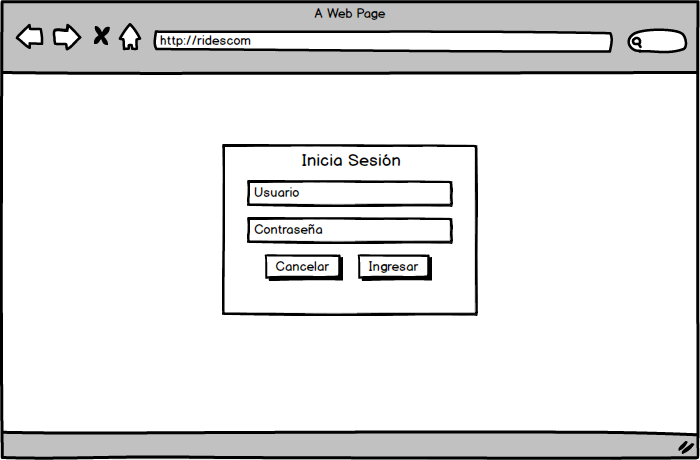
\includegraphics[width=10cm, height=6cm]{Imagenes/Nuevos/P1_LoginJFD_coord}
			\caption{Inicio sesión para el JFD y el coordinador de U.A.}
			\label{inicioJFDycoord}
		\end{figure}
		\pagebreak
		
		\begin{figure}[hbt!]
			\centering
			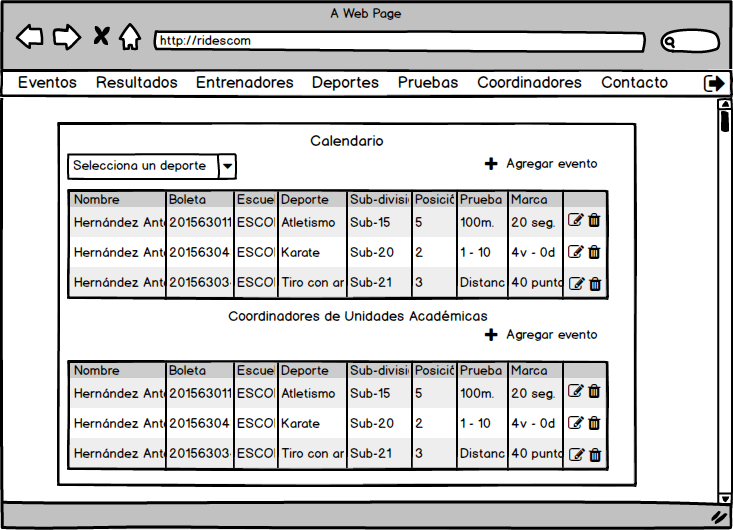
\includegraphics[width=10cm, height=6cm]{Imagenes/Nuevos/P2_Inicio_JefeFD}
			\caption{Página principal para el Jefe de Fomento Deportivo}
			\label{principalJFD}
		\end{figure}
	
		\begin{figure} [hbt!]
			\centering
			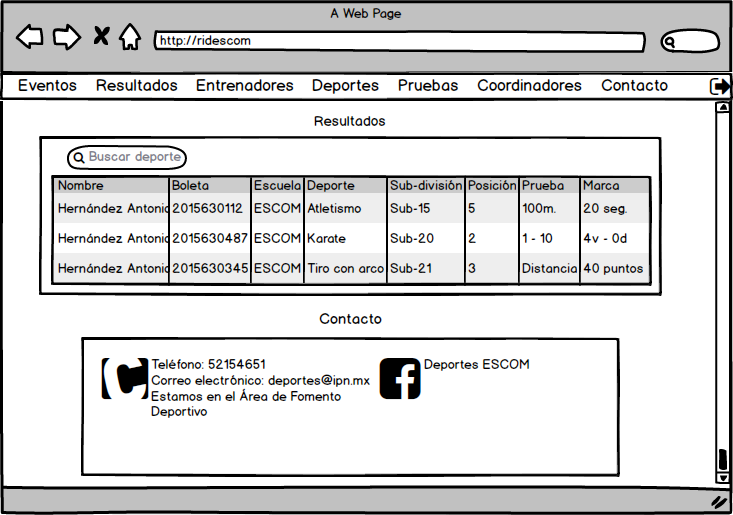
\includegraphics[width=10cm, height=6cm]{Imagenes/Nuevos/P3_Inicio_JefeFD1}
			\caption{Página principal para el Jefe de Fomento (Continuación).}
			\label{principalJFD1}
		\end{figure}
	
		\begin{figure} [hbt!]
			\centering
			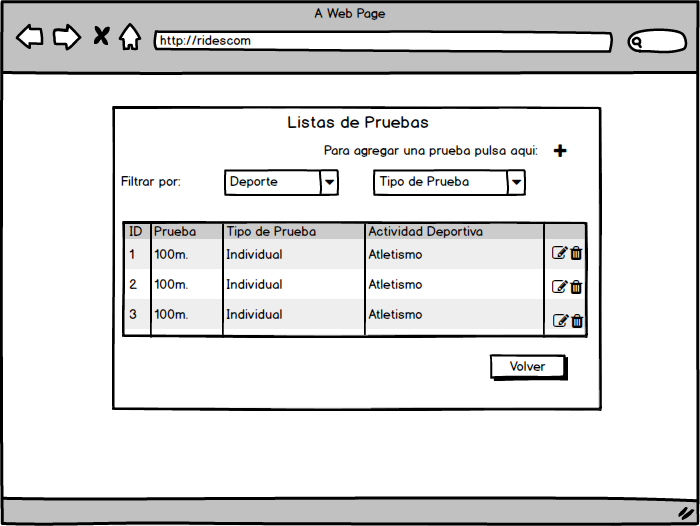
\includegraphics[width=10cm, height=6cm]{Imagenes/Nuevos/P25_Pruebas_JFD}
			\caption{Página para visualizar las pruebas dadas de alta. (Jefe de Fomento Deportivo)}
			\label{pruebas}
		\end{figure}
		\pagebreak
		
		\begin{figure} [hbt!]
			\centering
			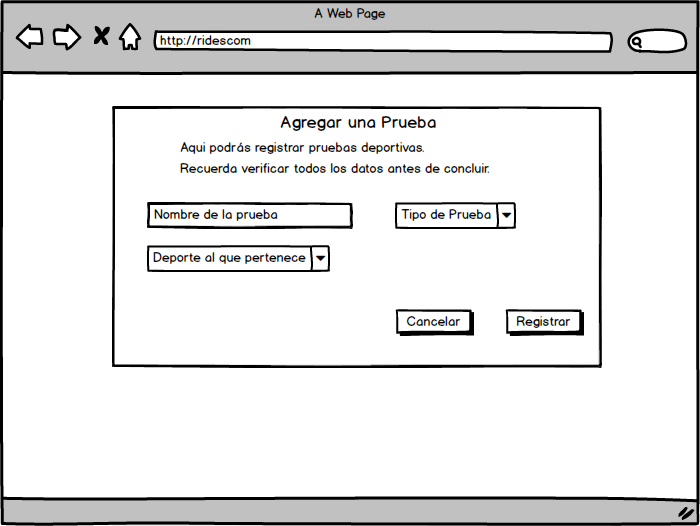
\includegraphics[width=10cm, height=6cm]{Imagenes/Nuevos/P26_AgregarPruebas_JFD}
			\caption{Página para agregar las distintas pruebas pruebas. (Jefe de Fomento Deportivo)}
			\label{agregarpruebas}
		\end{figure}
		
		\begin{figure} [hbt!]
			\centering
			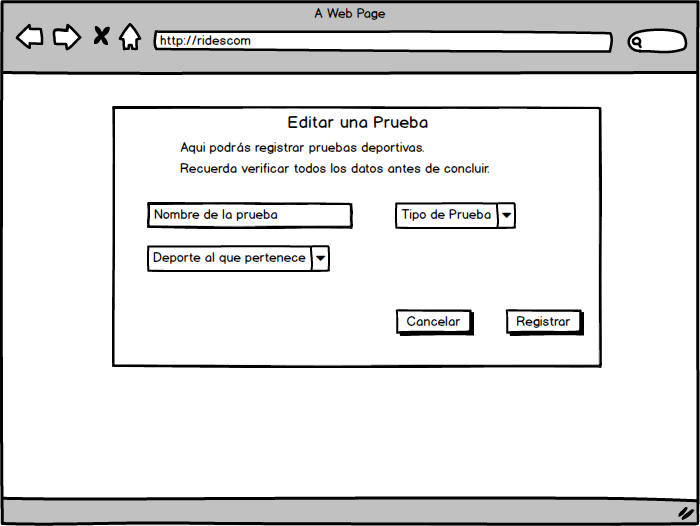
\includegraphics[width=10cm, height=6cm]{Imagenes/Nuevos/P26_EditarPruebas_JFD}
			\caption{Página para editar los datos de las pruebas previamente registrados. (Jefe de Fomento Deportivo)}
			\label{editarpruebas}
		\end{figure}
	
		\begin{figure} [hbt!]
			\centering
			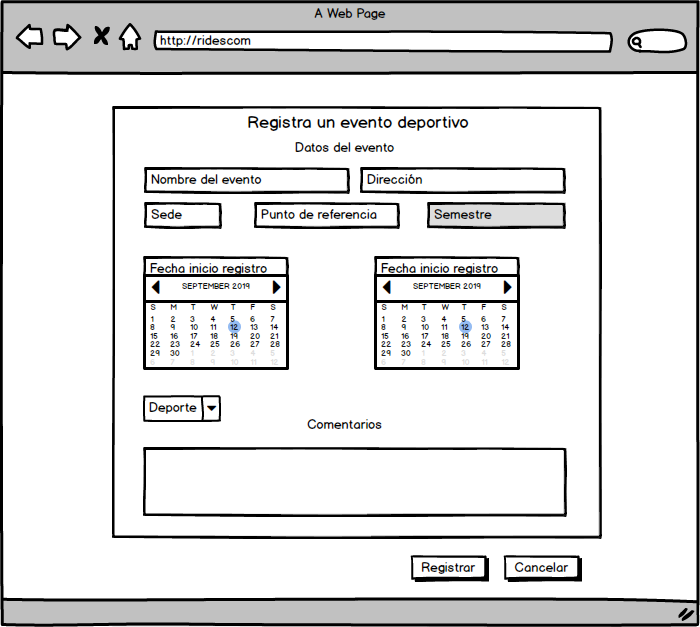
\includegraphics[width=10cm, height=6cm]{Imagenes/Nuevos/P4_Crear_evento_deportivo}
			\caption{Vista para dar de alta un evento deportivo (Jefe de Fomento Deportivo).}
			\label{creaevento}
		\end{figure}
		\pagebreak	
		
		\begin{figure} [hbt!]
			\centering
			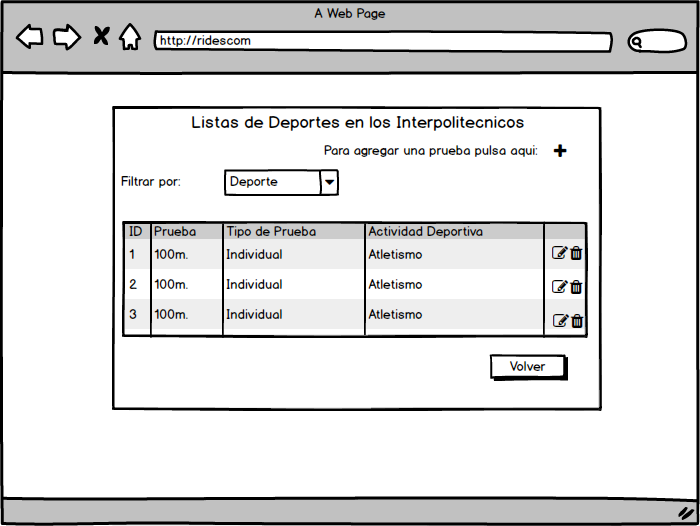
\includegraphics[width=10cm, height=6cm]{Imagenes/Nuevos/P27_Deportes_JFD}
			\caption{Página para visualizar los deportes que se llevaran a cabo en los eventos interpolitécnicos}
			\label{deportes}
		\end{figure}
	
		\begin{figure} [hbt!]
			\centering
			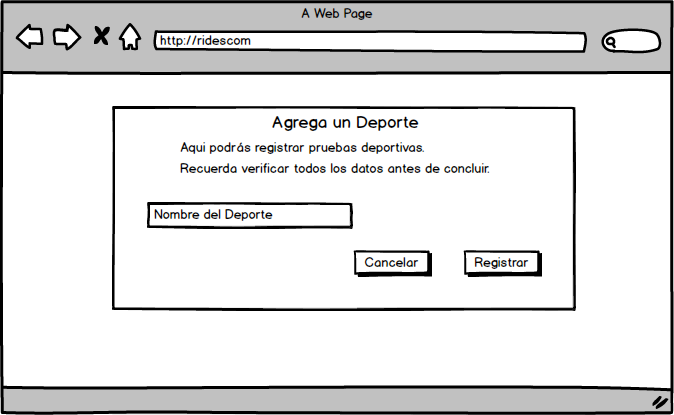
\includegraphics[width=10cm, height=6cm]{Imagenes/Nuevos/P28_AgregarDeportes_JFD}
			\caption{Página para agregar un deporte.}
			\label{agregadeporte}
		\end{figure}
		
		\begin{figure} [hbt!]
			\centering
			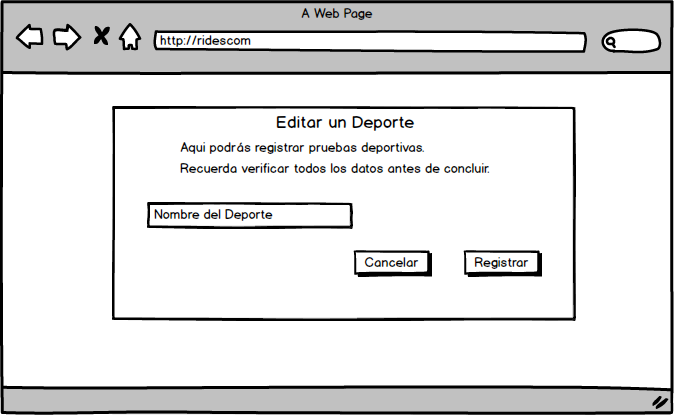
\includegraphics[width=10cm, height=6cm]{Imagenes/Nuevos/P29_EditarDeportes_JFD}
			\caption{Página para editar datos de los deportes}
			\label{editardeporte}
		\end{figure}
		\pagebreak
		
		\begin{figure} [hbt!]
			\centering
			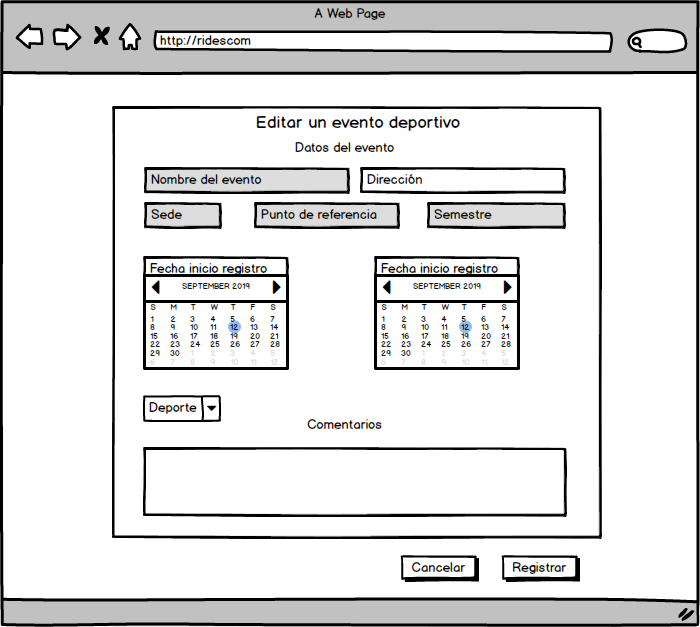
\includegraphics[width=10cm, height=6cm]{Imagenes/Nuevos/P5_Editar_evento_deportivo}
			\caption{Vista para editar datos de un evento ya registrado. (Jefe de FOmento Deportivo).}
			\label{editarevento}
		\end{figure}
	
		\begin{figure} [hbt!]
			\centering
			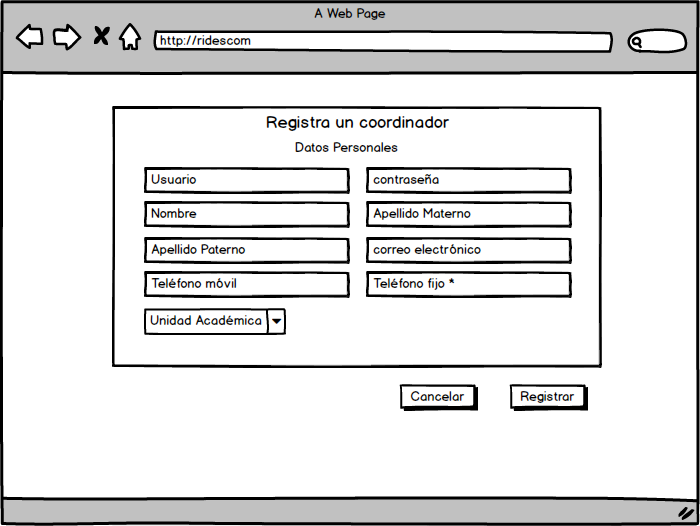
\includegraphics[width=10cm, height=6cm]{Imagenes/Nuevos/P6_Registro_coordinador}
			\caption{Vista para registrar un coordinador de unidad académica. (Jefe de Fomento Deportivo).}
			\label{registrarcoord}
		\end{figure}
		
		\begin{figure} [hbt!]
			\centering
			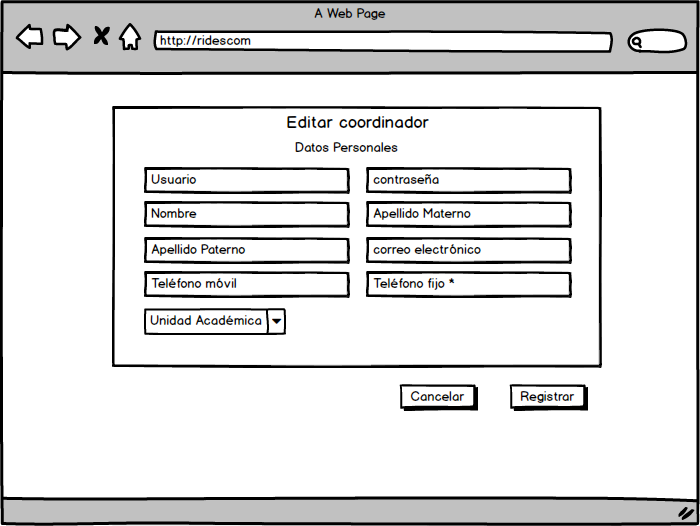
\includegraphics[width=10cm, height=6cm]{Imagenes/Nuevos/P7_Editar_coordinador}
			\caption{Vista para editar datos de un coordinador previamente registrado. (Jefe de Fomento Deportivo).}
			\label{editarcoord}
		\end{figure}
\pagebreak

		\begin{figure} [hbt!]
			\centering
			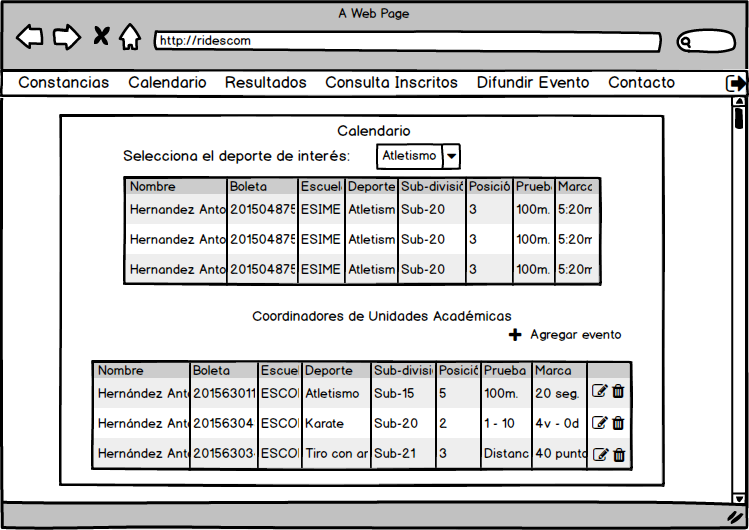
\includegraphics[width=10cm, height=6cm]{Imagenes/Nuevos/P8_Inicio_CoordUA}
			\caption{Vista principal para el coordinador de una Unidad Académica.}
			\label{principalcoord}
		\end{figure}
	
		\begin{figure} [hbt!]
			\centering
			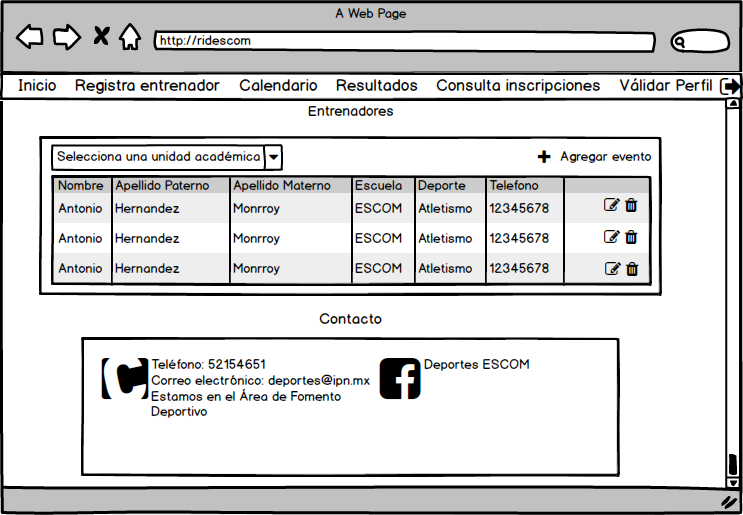
\includegraphics[width=10cm, height=6cm]{Imagenes/Nuevos/P9_Inicio_CoordUA1}
			\caption{Vista principal para el coordinador de una Unidad Académica (Continuación).}
			\label{principalcoord1}
		\end{figure}
	\pagebreak
		
		\begin{figure} [hbt!] 
			\centering
			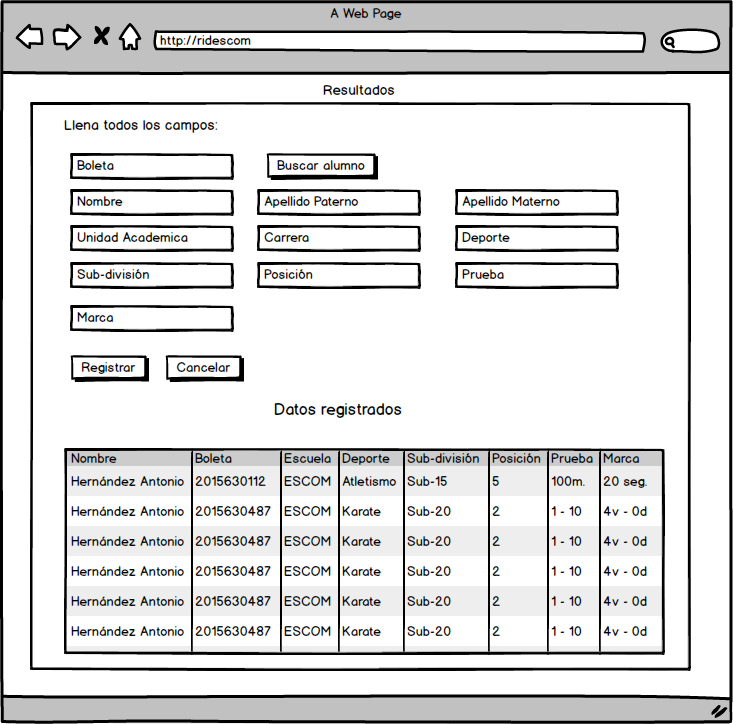
\includegraphics[width=10cm, height=7cm]{Imagenes/Nuevos/P10_Ingresa_resultados}
			\caption{Vista para ingresar los resultados obtenidos por los participantes (Coordinador de Unidad Académica).}
			\label{ingresaresultados}
		\end{figure}
		
		\begin{figure} [hbt!]
			\centering
			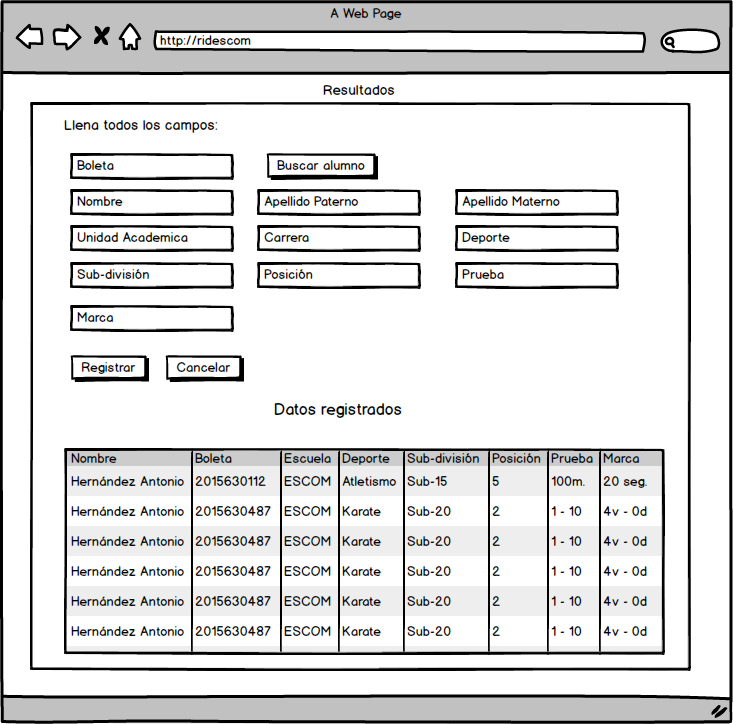
\includegraphics[width=10cm, height=7cm]{Imagenes/Nuevos/P11_Editar_resultados}
			\caption{Vista para editar los resultados de los participantes (Coordinador de Unidad Académica).}
			\label{editaresultados}
		\end{figure}
		\pagebreak
		
		\begin{figure} [hbt!]
			\centering
			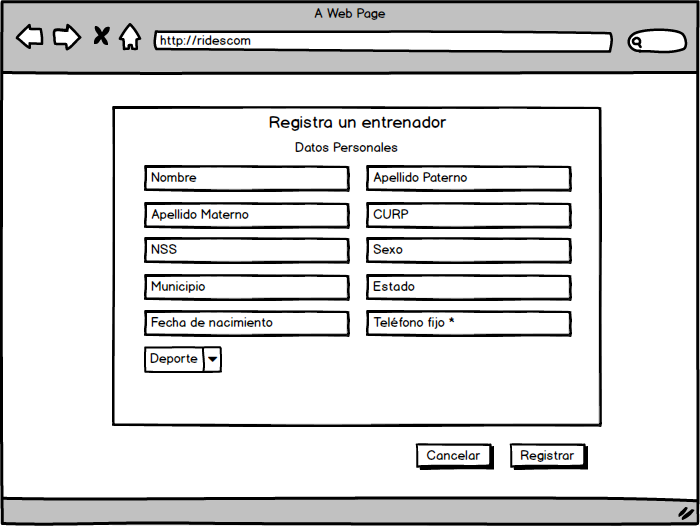
\includegraphics[width=10cm, height=6cm]{Imagenes/Nuevos/P12_Registro_entrenador}
			\caption{Vista para registrar a un entrenador (Coordinador de Unidad Académica).}
			\label{registroentrenador}
		\end{figure}
		
		\begin{figure} [hbt!]
			\centering
			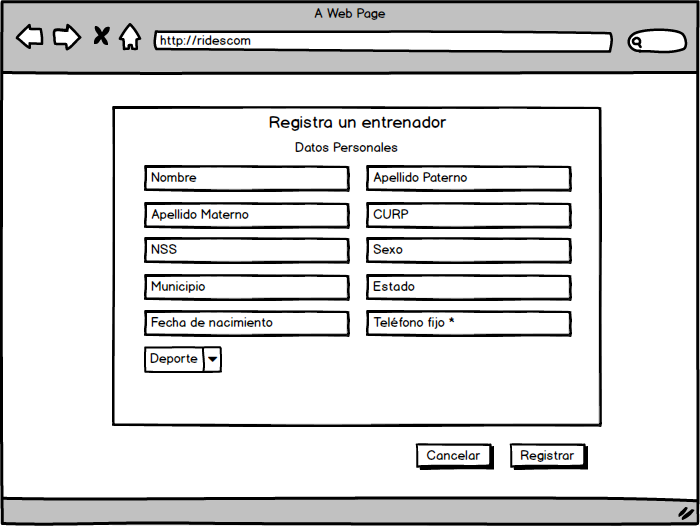
\includegraphics[width=10cm, height=6cm]{Imagenes/Nuevos/P13_Editar_entrenador}
			\caption{Vista para editar los datos del entrenador (Coordinador de Unidad Académica).}
			\label{editarentrenador}
		\end{figure}
		
		\begin{figure} [hbt!]
			\centering
			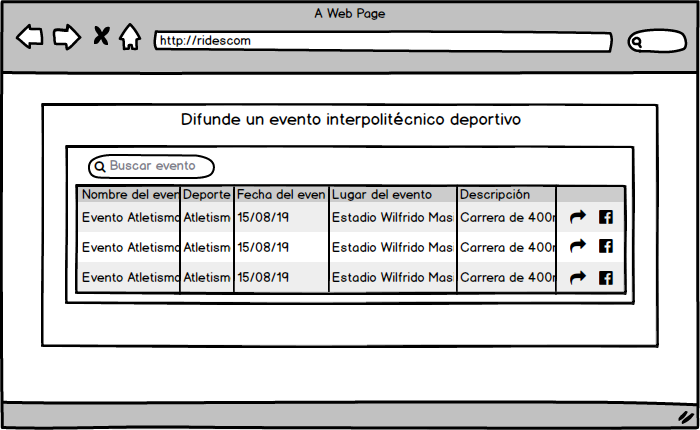
\includegraphics[width=10cm, height=6cm]{Imagenes/Nuevos/P14_Difundir_evento}
			\caption{Vista para difundir un evento interpolitécnico deportivo (Coordinador de Unidad Académica).}
			\label{difundirevento}
		\end{figure}
		\pagebreak

		\begin{figure} [hbt!]
			\centering
			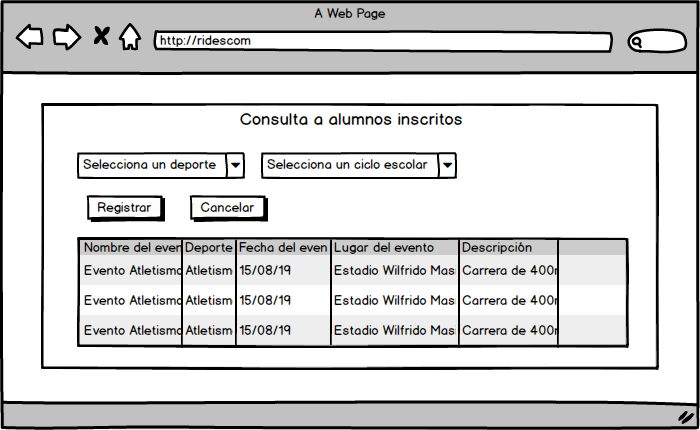
\includegraphics[width=10cm, height=6cm]{Imagenes/Nuevos/P15_Consulta_alumnos_inscritos}
			\caption{Vista para consultar los alumnos que se han inscrito a un evento (Coordinador de Unidad Académica).}
			\label{consultaalumnosinscritos}
		\end{figure}
	
		\begin{figure} [hbt!]
			\centering
			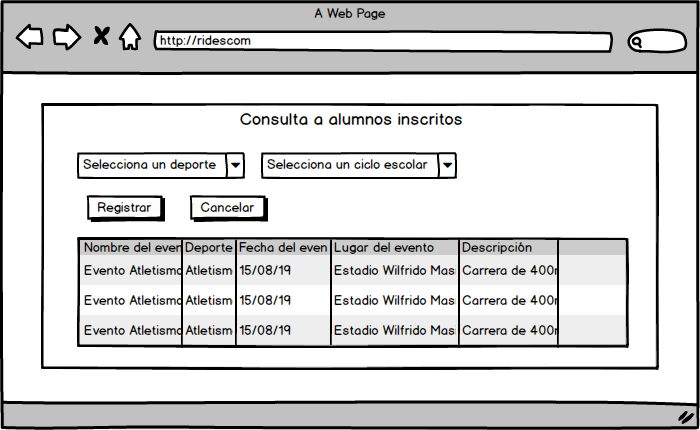
\includegraphics[width=10cm, height=6cm]{Imagenes/Nuevos/P16_Consulta_para_expedir_constancias}
			\caption{Vista para consultar participación de alumnos (Coordinador).}
			\label{consultaparaexpedirconstancias}
		\end{figure}
		
		\begin{figure} [hbt!]
			\centering
			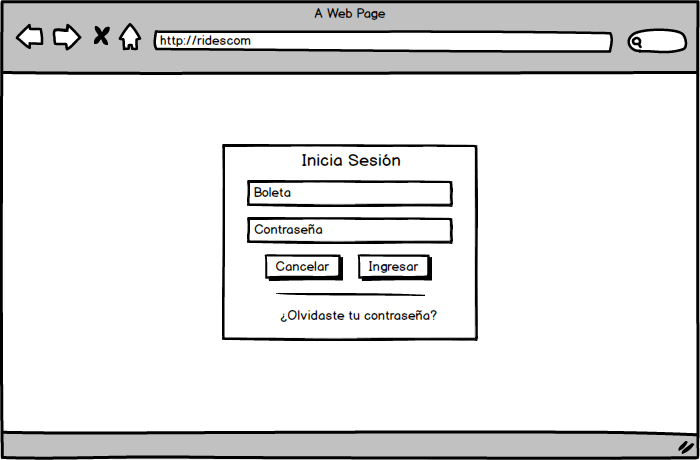
\includegraphics[width=10cm, height=6cm]{Imagenes/Nuevos/P17_Login_alumno}
			\caption{Vista Inicio de Sesión para el alumno.}
			\label{loginalumno}
		\end{figure}
	\pagebreak
		
		\begin{figure} [hbt!]
			\centering
			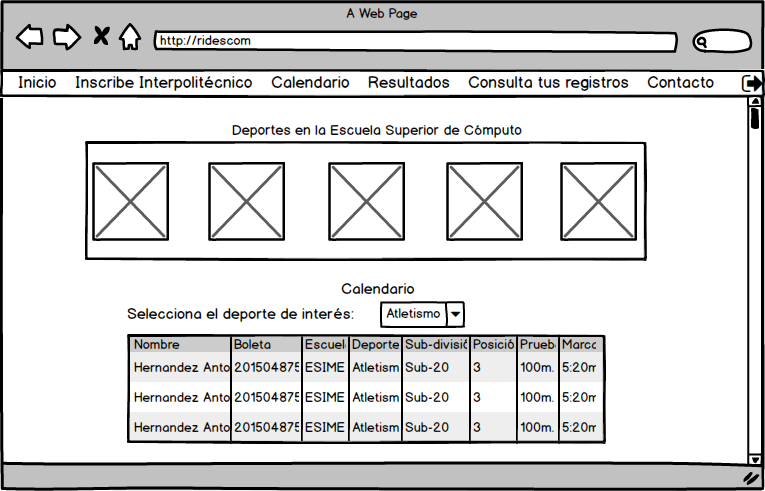
\includegraphics[width=10cm, height=6cm]{Imagenes/Nuevos/P18_Inicio_paticipante}
			\caption{Vista principal del alumno.}
			\label{principalalum}
		\end{figure}
		
		\begin{figure} [hbt!]
			\centering
			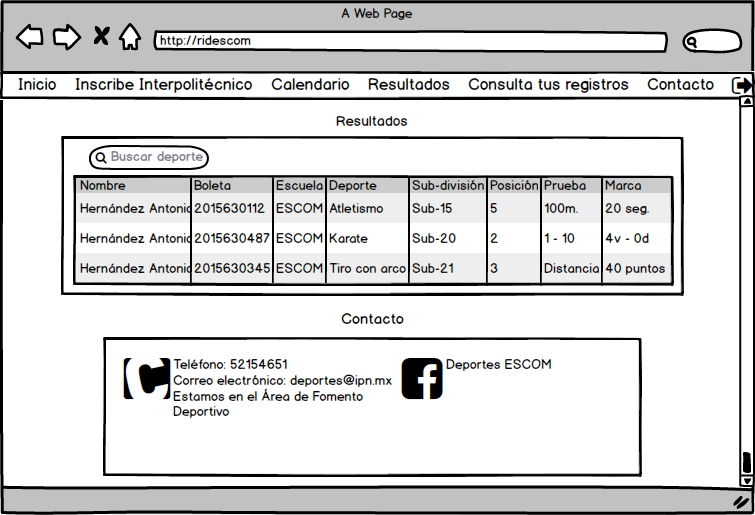
\includegraphics[width=10cm, height=6cm]{Imagenes/Nuevos/P19_Inicio_paticipante1}
			\caption{Vista principal del alumno (Continuación).}
			\label{principalalum1}
		\end{figure}
	
		\begin{figure} [hbt!]
			\centering
			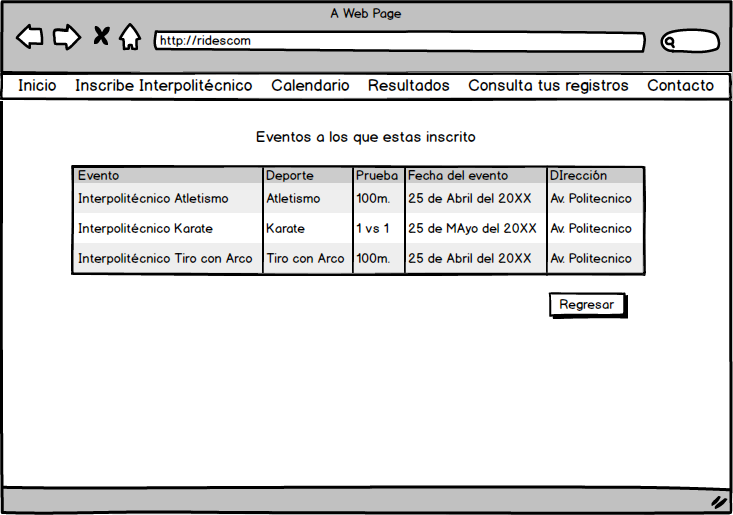
\includegraphics[width=10cm, height=6cm]{Imagenes/Nuevos/P20_Consulta_Inscripciones}
			\caption{Vista para consultar los eventos a los que se a registrado el alumno (Alumno).}
			\label{consultainscripcion}
		\end{figure}
	\pagebreak
		
		\begin{figure} [hbt!]
			\centering
			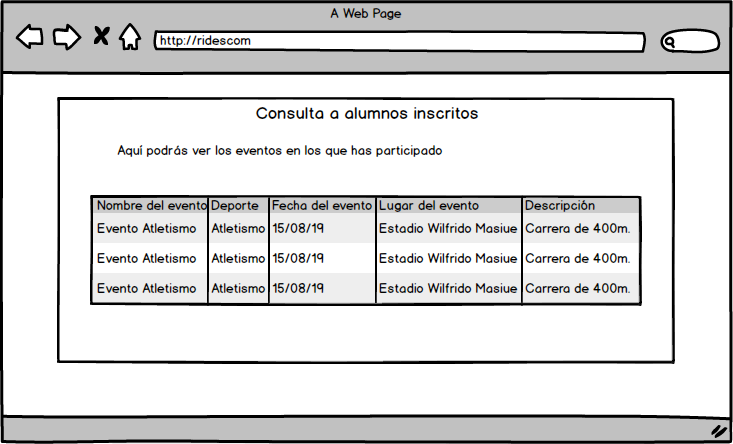
\includegraphics[width=10cm, height=6cm]{Imagenes/Nuevos/P21_Historial}
			\caption{Vista para que el alumno pueda visualizar todos los eventos en los que ha participado.}
			\label{historial}
		\end{figure}

	\chapter{Apartado D: Diagrama de Procesos}	
		
		\begin{figure}[hbt!]
			\centering
			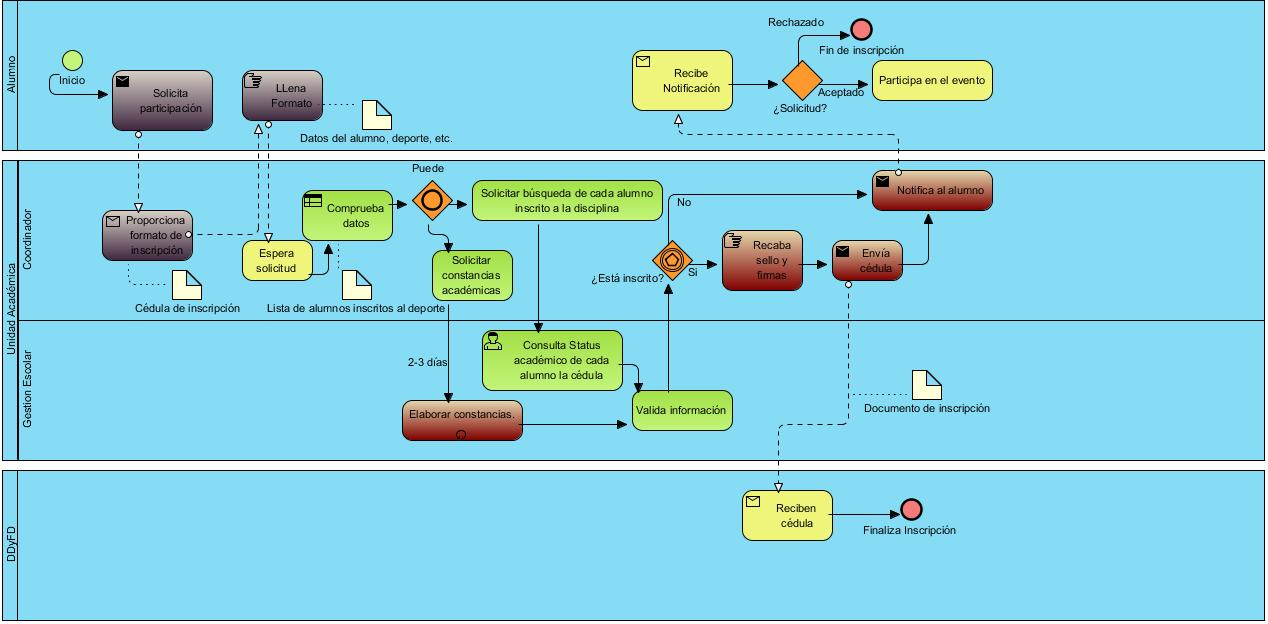
\includegraphics[width=16cm, height=8cm]{Imagenes/Disenos/ProcesoInscripcionActual.jpg}
			\caption{Proceso actual para la inscripcion a un evento interpolitécnico deportivo.}
			\label{ProcesoInscripcionActual}
		\end{figure}
	\pagebreak
	
		\begin{figure}[hbt!]
			\centering
			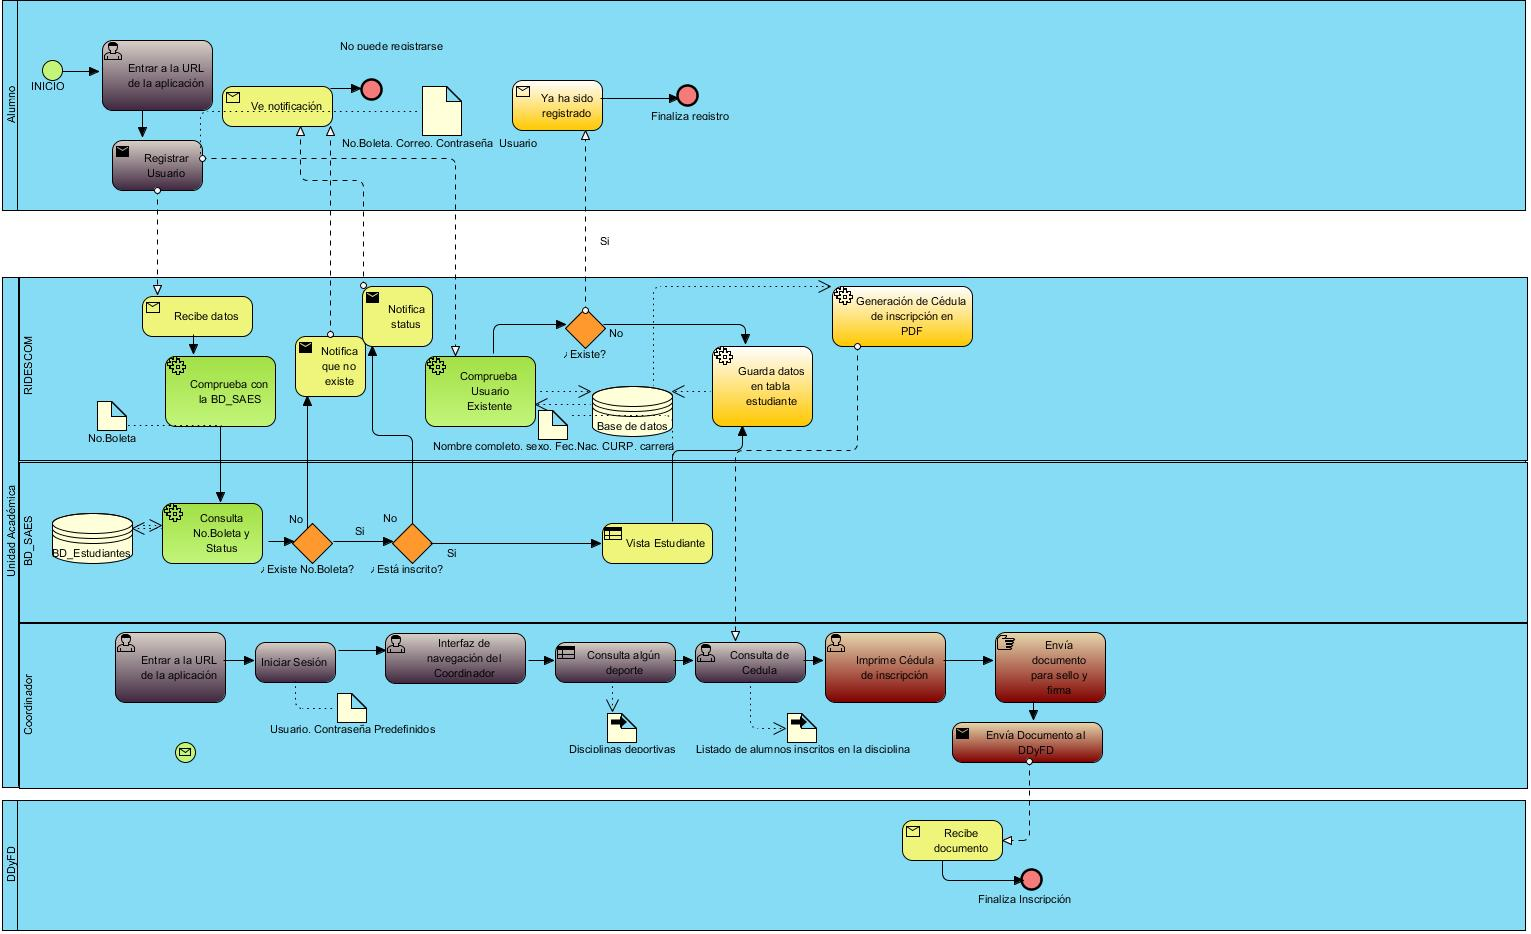
\includegraphics[width=16cm, height=8cm]{Imagenes/Disenos/ProcesoInscripcionPropuesto.jpg}
			\caption{Proceso propuesto para la inscripcion a un evento interpolitécnico deportivo.}
			\label{ProcesoInscripcionPropuesto}
		\end{figure}
	
	
	\chapter{Apartado E: Diagramas de Casos de Uso}
		\begin{figure}[hbt!]
			\centering
			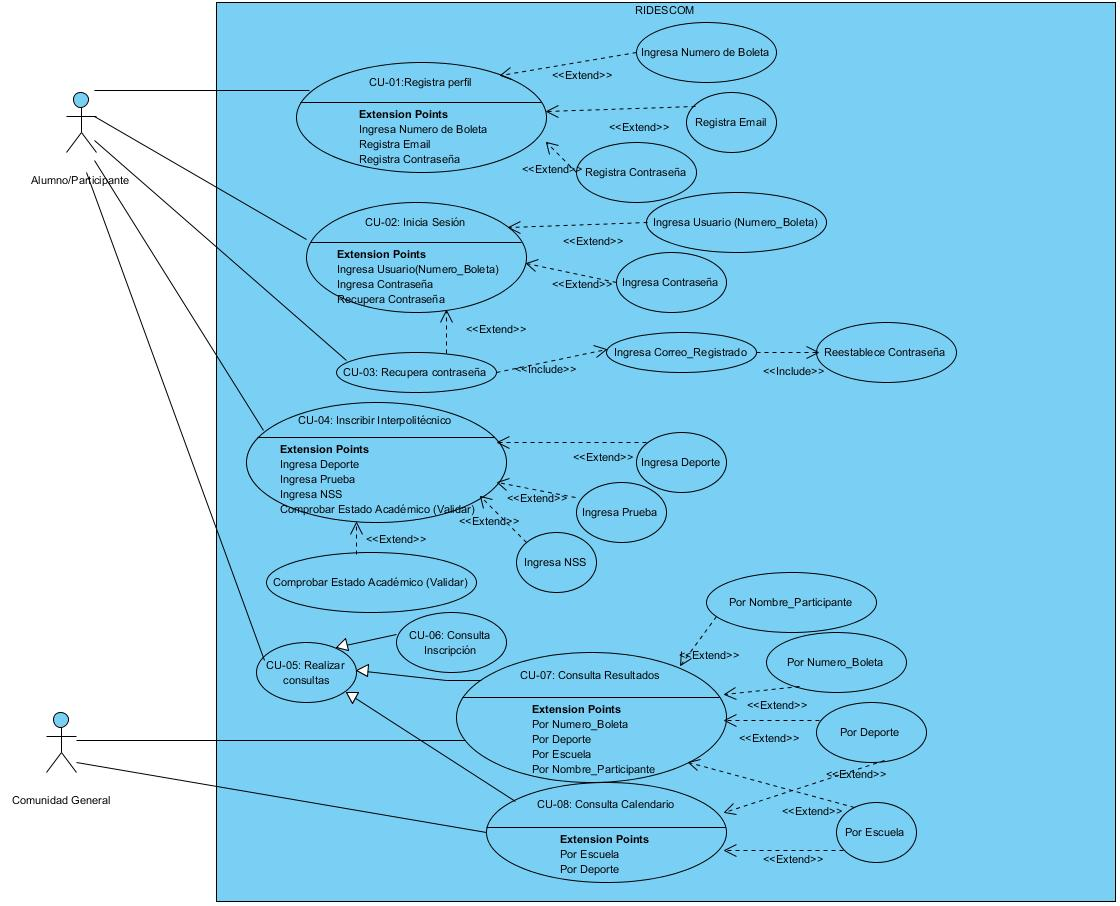
\includegraphics[width=16cm, height=8cm]{Imagenes/Disenos/DiagramasCU/Alumno.jpg}
			\caption{Diagrama de procesos Inscripción actual para un evento interpolitécnico deportivo.}
			\label{Inscripcion}
		\end{figure}
	\pagebreak
		\begin{figure}[hbt!]
			\centering
			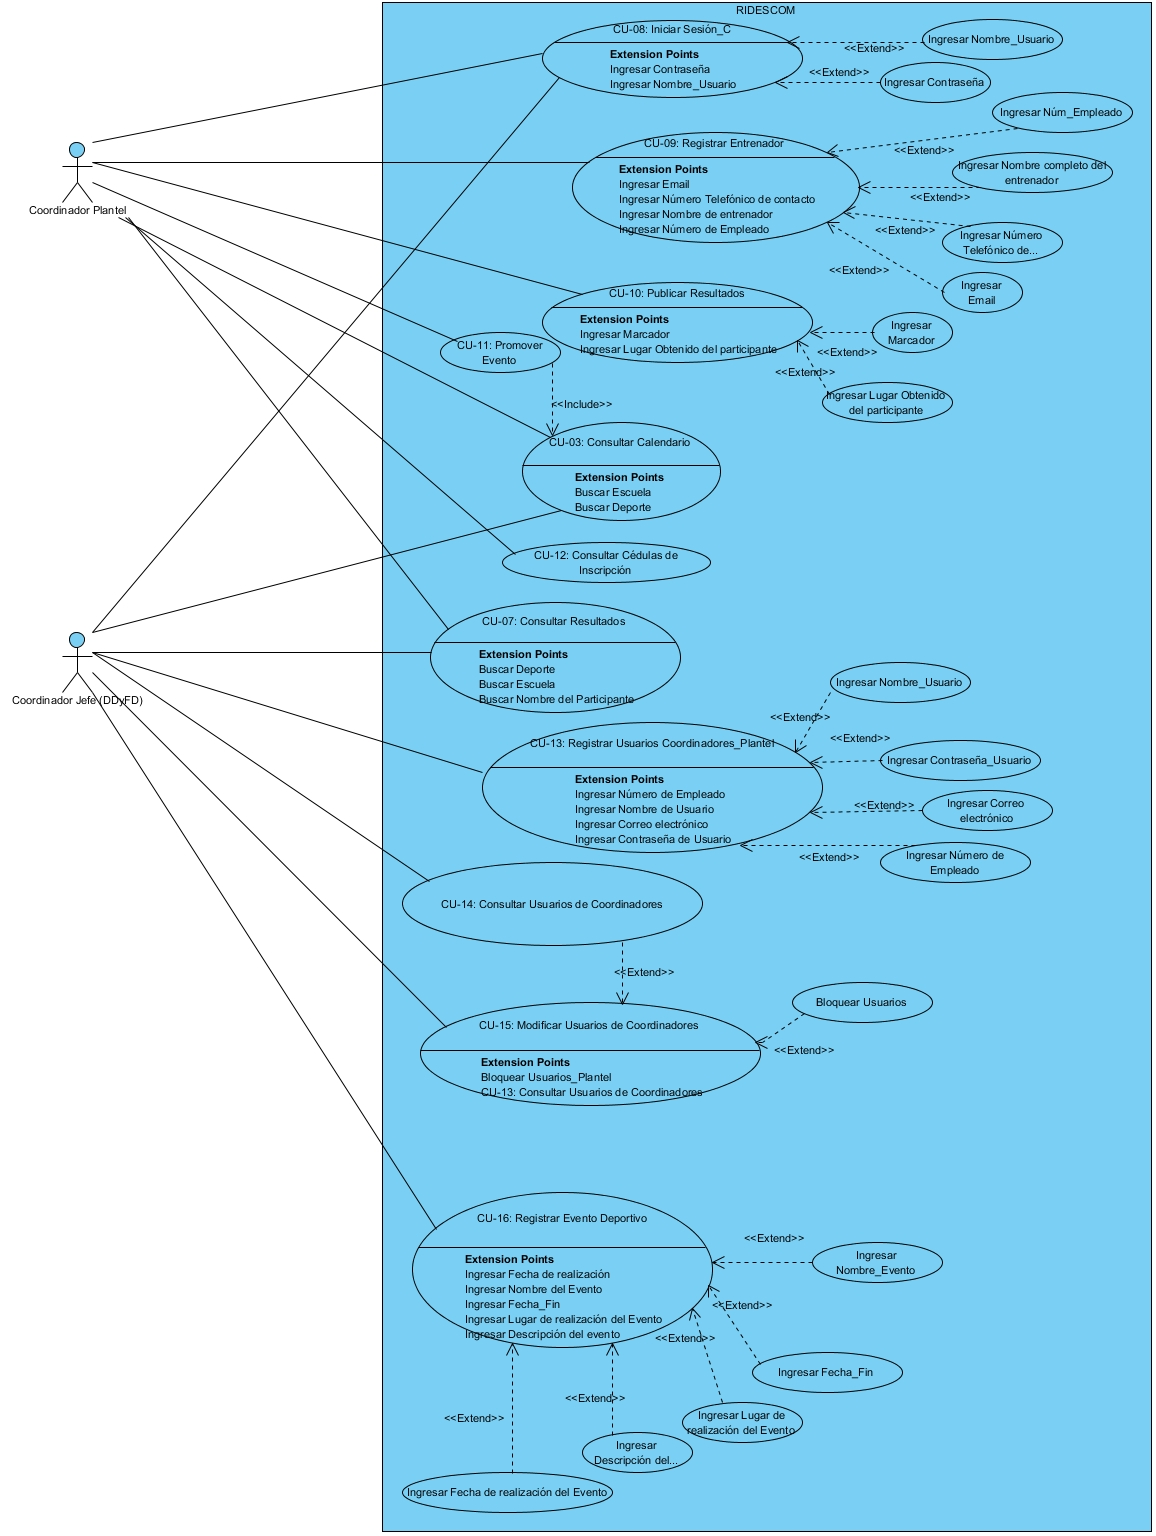
\includegraphics[width=16cm, height=12cm]{Imagenes/Disenos/DiagramasCU/CoordinadoresFinal.jpg}
			\caption{Diagrama de procesos Inscripción propuesto para un evento interpolitécnico deportivo.}
			\label{Inscripcion}
		\end{figure}
	
	\chapter{Apartado F: Crawler}
		\label{crawler}
	

	\chapter{Apartado G: Casos de Uso}
		\label{CasosdeUso}
		\begin{UseCase}{CU1}{Iniciar Sesión Jefe de Fomento Deportivo}{
		\noindent Esta caso de uso servirá para que el Jefe de Fomento Deportivo pueda ingresar a la página web, poder identificar al usuario y así mostrar las vistas que tienen asginada. \\
    	Para poder iniciar sesión el actor deberá oprimir el botón \IUbutton{ Iniciar Sesión } ubicado en la pantalla \ref{inicioJFDycoord}. Ingresará su número de boleta, contraseña el cual usa para ingresar al SAES (Sistema de Administración Escolar), y el captcha, como se muestra en la pantalla... Si los datos que ingresa no coinciden se le mostrará un mensaje.
        Una vez que incie sesión se le mostrará la pantalla principal.
        \MSGref{MSG1}{Campos requeridos}.
        
	} \label{CU1_Iniciarsesion}
		\UCitem{Versión}{0.1}
		\UCitem{Autor}{Rosales González Carlos Andrés}
		\UCitem{Supervisa}{Mendoza García Bruno Alejandro}
		\UCitem{Actor}{Jefe de Fomento Deportivo}
		\UCitem{Propósito}{Tener control de las personas registradas.}
        \UCitem{Precondiciones}{
        \begin{itemize}
            \item Contar con una cuenta.
            \item Contar con la contraseña.
        \end{itemize}}
        \UCitem{Postcondiciones}{Se muestra la pantalla principal}
		\UCitem{Entradas}{
        \begin{itemize}
        	\item Usuario. 
        	\item Contraseña
        \end{itemize}}
		\UCitem{Origen}{Pantalla, Teclado}
		\UCitem{Salidas}{
		\begin{itemize}
		    \item Acceso a la página principal del Jefe de Fomento Deportivo
		\end{itemize}}
		\UCitem{Destino}{Pantalla}
		\UCitem{Errores}{
        	\begin{itemize}
        	    \item Los campos están vacíos.
            	\item Usuario y/o contraseña incorrecta.
            \end{itemize}
       }
		\UCitem{Observaciones}{}
		\end{UseCase}
	\newpage
	
    \begin{UCtrayectoria}{Principal}
    \UCpaso[\UCactor] Ingresa a la página RIDESCOM.
    \UCpaso Muestra la pantalla \IUref{}{Pantalla de Inicio de Sesión \ref{inicioJFDycoord}}.
    \UCpaso[\UCactor] Oprime el botón \IUbutton{ JFD o Coordinador } que esta en la \IUref{}{Pantalla de Inicio de Sesión \ref{inicioJFDycoord}}.
    \UCpaso Muestra la \IUref{}{Pantalla de Inicio de Sesión \ref{inicioJFDycoord}}
	\UCpaso[\UCactor] Introduce Usuario y contraseña. \label{CU1_regresar} 
    \UCpaso[\UCactor] Presiona el botón \IUbutton{ Ingresar }.
    \UCpaso Comprueba que los campos no estén vacíos. \Trayref{A}
    \UCpaso Obtiene los valores ingresados
    \UCpaso Válida campos. \Trayref{B}
    \UCpaso Muestra la \IUref{}{Pantalla principal del Jefe de Fomento Deportivo. \ref{principalJFD}}
    \end{UCtrayectoria}
    
    \begin{UCtrayectoriaA}{A}{Campo(s) vacios}
    	\UCpaso muestra mensaje “CamposNecesario".
    	\UCpaso Continua en el paso \ref{CU1_regresar} del \UCref{CU1}.
    \end{UCtrayectoriaA}

	\begin{UCtrayectoriaA}{B}{Boleta y/o contraseña erróneo}
		\UCpaso muestra mensaje “El usuario y/o contraseña que se ingresó son erróneos”. Mensaje .
   		\UCpaso Continua en el paso \ref{CU1_regresar} del \UCref{CU1}.
	\end{UCtrayectoriaA}

	



		\begin{UseCase}{CU1.1}{Inicio Sesión}{
		Servirá para que el alumno pueda ingresar a la aplicación y así poder inscribirse en algún evento de su interés o consultar los eventos a los que ya se ha registrado previamente. \\
        En caso de que el alumno ingrese una boleta la cual no a sido registrada, se mostrará un mensaje el cual le indique que la boleta que ingreso no existe. Mensaje . De igual manera, si la contraseña es diferente a la que se registro aparecerá un mensaje que le indique que la contraseña no coincide. Mensaje .
	}
		\UCitem{Versión}{0.1}
		\UCitem{Autor}{Rosales González Carlos Andrés}
		\UCitem{Supervisa}{Mendoza García Bruno Alejandro}
		\UCitem{Actor}{Alumno}
		\UCitem{Propósito}{Tener control de las personas registradas.}
        \UCitem{Precondiciones}{
        \begin{itemize}
            \item Haberse registrado
            \item Perfil valido por el coordinador
        \end{itemize}}
        \UCitem{Postcondiciones}{Ninguna}
		\UCitem{Entradas}{
        \begin{itemize}
        	\item Número de boleta 
        	\item Contraseña
        \end{itemize}}
		\UCitem{Origen}{Pantalla, Teclado}
		\UCitem{Salidas}{
		\begin{itemize}
		    \item Acceso a la página principal del alumno
		\end{itemize}}
		\UCitem{Destino}{Pantalla}
		\UCitem{Errores}{
        	\begin{itemize}
        	    \item Los campos están vacíos.
            	\item No existe la boleta. Mensaje .
            	\item Contraseña incorrecta. Mensaje .
            \end{itemize}
       }
		\UCitem{Observaciones}{}
		\end{UseCase}
    \begin{UCtrayectoria}{Principal}
    \UCpaso[\UCactor] Oprime el botón Iniciar Sesión en la pantalla.
    \UCpaso Muestra la pantalla.
	\UCpaso[\UCactor] Introduce Boleta y contraseña. 
    \UCpaso[\UCactor] Presiona el botón Ingresar.
    \UCpaso Comprueba que los campos no estén vacíos. \Trayref{A} \Trayref{B} \Trayref{C}
    \UCpaso Obtiene los valores ingresados
    \UCpaso Válida campos. 
    \UCpaso Muestra la pantalla .
    \end{UCtrayectoria}
    
	\begin{UCtrayectoriaA}{A}{No hay dato insertado en el campo solicitado}
		\UCpaso muestra mensaje “Error: Los campos están vacíos por favor asegúrese de poner lo que se pide”. Mensaje .
		\UCpaso Regresa al paso 3 de la Trayectoria Principal.
	\end{UCtrayectoriaA}
	
	\begin{UCtrayectoriaA}{B}{}
		\UCpaso muestra mensaje “No existe boleta ingresada”. Mensaje .
		\UCpaso Regresa al paso 2 de la trayectoria principal.
	\end{UCtrayectoriaA}
	
	\begin{UCtrayectoriaA}{C}{}
		\UCpaso muestra mensaje “Contraseña incorrecta”. Mensaje .
		\UCpaso Regresa al paso 2 de la trayectoria principal.
	\end{UCtrayectoriaA}
		\begin{UseCase}{CU3}{Inscribir a un evento interpolitécnico deportivo}{
		\noindent Este caso de uso permite que el actor alumno, pueda registrarse en el evento interpolitécnico deportivo de su interés. Deberá llenar un formulario donde se solicitan datos del alumno como: Grupo, NSS (Número de Seguro Social), correo electrónico, Delegación/Municipio, así como el seleccionar el deporte en el que desea participar.\\
        Para poder inscribirse, deberá primero validar su estatus académico (Inscrito/No inscrito), para ello debe ingresar su boleta, contraseña y el captcha como se muestra en la pantalla \IUref{p15InscripcionInterpolitecnico1}{Pantalla Inscribir interpolitécnico 1.}, da click en el botón \IUbutton { Verificar } si cumple con el requisito, continua el proceso, en caso contrario no podrá inscribirse en algun evento interpolitécnico deportivo.\\
        El siguiente paso es la verificación de datos como se muestra en la pantalla \IUref{p15InscripcionInterpolitecnico2}{Pantalla Inscribir interpolitécnico 2.}, si los datos son correctos da click en el botón \IUbutton{ Aceptar }\\
        Si los datos son correctos, da click en el botón \IUbutton{ Aceptar }, a continuación se muestra la pantalla \IUref{p15InscripcionInterpolitecnico3}{Pantalla Inscribir interpolitécnico 3.} donde llenará los datos corresponidentes al evento deportivo. Una vez que se llenen todos los campos, el alumno da click en el botón \IUbutton{ Inscribir }.\\ 
        Al final se mostrará un mensaje de confirmación de la inscripción.
	}
		\UCitem{Versión}{0.1}
		\UCitem{Autor}{Rosales González Carlos Andrés}
		\UCitem{Supervisa}{Mendoza García Bruno Alejandro}
		\UCitem{Actor}{Alumno}
		\UCitem{Propósito}{Poder participar en un evento deportivo.}
        \UCitem{Precondiciones}{
        \begin{itemize}
            \item Iniciar Sesión
            \item Ser un alumno pertenenciente al IPN
            \item Validar estatus académico
        \end{itemize}}
        \UCitem{Postcondiciones}{Persitencia de dat}
		\UCitem{Entradas}{
        \begin{itemize}
        	\item Boleta, contraseña y captcha
        	\item Grupo, Escuela, Carrera
        	\item Nombre, Apellido, Sexo
        	\item Curp, Fecha de nacimiento, Lugar
        	\item NSS, Correo electrónico, Delegación
        	\item Deporte, Sub-division, Prueba, Fecha del evento
        \end{itemize}}
		\UCitem{Origen}{Teclado}
		\UCitem{Salidas}{
		\begin{itemize}
		    \item Confirmación de la inscripción al evento
		\end{itemize}}
		\UCitem{Destino}{Pantalla principal}
		\UCitem{Errores}{
        	\begin{itemize}
            	\item EL alumno no se encuentra inscrito en el periodo actual.
            	\item Completa todos los campos
            \end{itemize}
       }
		\UCitem{Observaciones}{}
		\end{UseCase}
    \begin{UCtrayectoria}{Principal}
    \UCpaso[\UCactor] Oprime el botón \IUbutton { Inscribir Interpolitécnico } de la pantalla \IUref{p13Iniciopaticipante}{Pantalla principal del alumno \ref{Inscripcioninterpolitecnico}}.\label{CU3_inicio}
    \UCpaso Muestra la pantalla \IUref{p15InscripcionInterpolitecnico1}{Pantalla Inscribir interpolitécnico 1 \ref{Inscripcioninterpolitecnico2}.}\label{CU3_regresa}
    \UCpaso[\UCactor] Ingresa boleta, contraseña y captcha.
    \UCpaso[\UCactor] Da click en el botón \IUbutton { Verificar }
    \UCpaso Envia los datos mediante el crawler a la página del SAES.
    \UCpaso Verifica si hay acceso al SAES. \Trayref{A} \Trayref{B}
    \UCpaso Muestra la pantalla \IUref{p15InscripcionInterpolitecnico2}{Pantalla Inscribir interpolitécnico 2 \ref{Inscripcioninterpolitecnico3}}.
    \UCpaso Muestra los datos personales del alumno.
	\UCpaso[\UCactor] Da click en el botón \IUbutton {Aceptar}. \Trayref{C}
	\UCpaso Busca los deportes y subdivisiones asociados a la unidad académica del alumno que esta haciendo la solicitud.
	\UCpaso Muestra la pantalla \IUref{p15InscripcionInterpolitecnico3}{Pantalla Inscribir interpolitécnico 3.}. \label{CU3_deporte}
	\UCpaso[\UCactor] Llena los campos solicitados. \Trayref{D}
    \UCpaso Confirma registro en una ventana emergente.
    \UCpaso Carga la pantalla Principal.
    \end{UCtrayectoria}
    
	\begin{UCtrayectoriaA}{A}{El alumno debe de estar inscrito para continuar.}
		\UCpaso Muestra el mensaje. “El alumno no esta inscrito en el periodo actual”
   		\UCpaso Continua en el paso \ref{CU3_regresa} del \UCref{CU3}.
	\end{UCtrayectoriaA}
	
	\begin{UCtrayectoriaA}{B}{El alumno cancela el proceso de Inscribir interpolitécnico}
		\UCpaso[\UCactor] Da click en el botón \IUbutton { Cancelar } de la pantalla \IUref{p15InscripcionInterpolitecnico1}{Pantalla Inscribir interpolitécnico 1.}
		\UCpaso  Continua en el paso \ref{CU3_inicio} del \UCref{CU3}.
	\end{UCtrayectoriaA}

	\begin{UCtrayectoriaA}{C}{Los datos del alumno no coinciden}
		\UCpaso[\UCactor] Da click en el botón \IUbutton { Cancelar } de la pantalla \IUref{p15InscripcionInterpolitecnico2}{Pantalla Inscribir interpolitécnico 2.}
		\UCpaso Continua en el paso \ref{CU3_inicio} del \UCref{CU3}.
	\end{UCtrayectoriaA}
	
	\begin{UCtrayectoriaA}{D}{El alumno no completa los campos requeridos}
		\UCpaso Muestra el mensaje "Debes llenar todos los campos solicitados". \ref{CU3_deporte}
		\UCpaso Continua en el paso \ref{CU3_inicio} del \UCref{CU3}.
	\end{UCtrayectoriaA}
		\begin{UseCase}{CU3}{Inscribir a un evento interpolitécnico deportivo}{
		\noindent Este caso de uso permite que el actor alumno, pueda registrarse en el evento interpolitécnico deportivo de su interés. Deberá llenar un formulario donde se solicitan datos del alumno como: Grupo, NSS (Número de Seguro Social), correo electrónico, Delegación/Municipio, así como el seleccionar el deporte en el que desea participar.\\
        Para poder inscribirse, deberá primero validar su estatus académico (Inscrito/No inscrito), para ello debe ingresar su boleta, contraseña y el captcha como se muestra en la pantalla \IUref{p15InscripcionInterpolitecnico1}{Pantalla Inscribir interpolitécnico 1.}, da click en el botón \IUbutton { Verificar } si cumple con el requisito, continua el proceso, en caso contrario no podrá inscribirse en algun evento interpolitécnico deportivo.\\
        El siguiente paso es la verificación de datos como se muestra en la pantalla \IUref{p15InscripcionInterpolitecnico2}{Pantalla Inscribir interpolitécnico 2.}, si los datos son correctos da click en el botón \IUbutton{ Aceptar }\\
        Si los datos son correctos, da click en el botón \IUbutton{ Aceptar }, a continuación se muestra la pantalla \IUref{p15InscripcionInterpolitecnico3}{Pantalla Inscribir interpolitécnico 3.} donde llenará los datos corresponidentes al evento deportivo. Una vez que se llenen todos los campos, el alumno da click en el botón \IUbutton{ Inscribir }.\\ 
        Al final se mostrará un mensaje de confirmación de la inscripción.
	}
		\UCitem{Versión}{0.1}
		\UCitem{Autor}{Rosales González Carlos Andrés}
		\UCitem{Supervisa}{Mendoza García Bruno Alejandro}
		\UCitem{Actor}{Alumno}
		\UCitem{Propósito}{Poder participar en un evento deportivo.}
        \UCitem{Precondiciones}{
        \begin{itemize}
            \item Iniciar Sesión
            \item Ser un alumno pertenenciente al IPN
            \item Validar estatus académico
        \end{itemize}}
        \UCitem{Postcondiciones}{Persitencia de dat}
		\UCitem{Entradas}{
        \begin{itemize}
        	\item Boleta, contraseña y captcha
        	\item Grupo, Escuela, Carrera
        	\item Nombre, Apellido, Sexo
        	\item Curp, Fecha de nacimiento, Lugar
        	\item NSS, Correo electrónico, Delegación
        	\item Deporte, Sub-division, Prueba, Fecha del evento
        \end{itemize}}
		\UCitem{Origen}{Teclado}
		\UCitem{Salidas}{
		\begin{itemize}
		    \item Confirmación de la inscripción al evento
		\end{itemize}}
		\UCitem{Destino}{Pantalla principal}
		\UCitem{Errores}{
        	\begin{itemize}
            	\item EL alumno no se encuentra inscrito en el periodo actual.
            	\item Completa todos los campos
            \end{itemize}
       }
		\UCitem{Observaciones}{}
		\end{UseCase}
    \begin{UCtrayectoria}{Principal}
    \UCpaso[\UCactor] Oprime el botón \IUbutton { Inscribir Interpolitécnico } de la pantalla \IUref{p13Iniciopaticipante}{Pantalla principal del alumno \ref{Inscripcioninterpolitecnico}}.\label{CU3_inicio}
    \UCpaso Muestra la pantalla \IUref{p15InscripcionInterpolitecnico1}{Pantalla Inscribir interpolitécnico 1 \ref{Inscripcioninterpolitecnico2}.}\label{CU3_regresa}
    \UCpaso[\UCactor] Ingresa boleta, contraseña y captcha.
    \UCpaso[\UCactor] Da click en el botón \IUbutton { Verificar }
    \UCpaso Envia los datos mediante el crawler a la página del SAES.
    \UCpaso Verifica si hay acceso al SAES. \Trayref{A} \Trayref{B}
    \UCpaso Muestra la pantalla \IUref{p15InscripcionInterpolitecnico2}{Pantalla Inscribir interpolitécnico 2 \ref{Inscripcioninterpolitecnico3}}.
    \UCpaso Muestra los datos personales del alumno.
	\UCpaso[\UCactor] Da click en el botón \IUbutton {Aceptar}. \Trayref{C}
	\UCpaso Busca los deportes y subdivisiones asociados a la unidad académica del alumno que esta haciendo la solicitud.
	\UCpaso Muestra la pantalla \IUref{p15InscripcionInterpolitecnico3}{Pantalla Inscribir interpolitécnico 3.}. \label{CU3_deporte}
	\UCpaso[\UCactor] Llena los campos solicitados. \Trayref{D}
    \UCpaso Confirma registro en una ventana emergente.
    \UCpaso Carga la pantalla Principal.
    \end{UCtrayectoria}
    
	\begin{UCtrayectoriaA}{A}{El alumno debe de estar inscrito para continuar.}
		\UCpaso Muestra el mensaje. “El alumno no esta inscrito en el periodo actual”
   		\UCpaso Continua en el paso \ref{CU3_regresa} del \UCref{CU3}.
	\end{UCtrayectoriaA}
	
	\begin{UCtrayectoriaA}{B}{El alumno cancela el proceso de Inscribir interpolitécnico}
		\UCpaso[\UCactor] Da click en el botón \IUbutton { Cancelar } de la pantalla \IUref{p15InscripcionInterpolitecnico1}{Pantalla Inscribir interpolitécnico 1.}
		\UCpaso  Continua en el paso \ref{CU3_inicio} del \UCref{CU3}.
	\end{UCtrayectoriaA}

	\begin{UCtrayectoriaA}{C}{Los datos del alumno no coinciden}
		\UCpaso[\UCactor] Da click en el botón \IUbutton { Cancelar } de la pantalla \IUref{p15InscripcionInterpolitecnico2}{Pantalla Inscribir interpolitécnico 2.}
		\UCpaso Continua en el paso \ref{CU3_inicio} del \UCref{CU3}.
	\end{UCtrayectoriaA}
	
	\begin{UCtrayectoriaA}{D}{El alumno no completa los campos requeridos}
		\UCpaso Muestra el mensaje "Debes llenar todos los campos solicitados". \ref{CU3_deporte}
		\UCpaso Continua en el paso \ref{CU3_inicio} del \UCref{CU3}.
	\end{UCtrayectoriaA}
		\begin{UseCase}{CU}{Registro}{
		Servirá para que el alumno que esté interesado en participar en algún evento interpolitécnico deportivo, cree una cuenta para posteriormente poder iniciar sesión y así, inscribirse en el evento de su interés. 
		Dicho registro lo encontrará dentro de la pantalla de Inicio en el apartado ‘Regístrate’, posteriormente deberá llenar los campos que se le solicitan, los cuales son: Boleta, Correo electrónico y una contraseña.
		El numero de Boleta consta de 10 caracteres numéricos, y en el correo solamente se aceptan los dominios más comunes (Gmail, Hotmail, Outlook).
		Una vez realizado, el alumno deberá acudir al Departamento de Actividades Deportivas de su Unidad Académica en un periodo no máximo a los 3 días a partir del día en el que se registró, para que el coordinador valide los datos que se ingresaron previamente. Para ello el coordinador deberá solicitar una identificación escolar vigente para corroborar dichos datos. }
		\label{CU_Registro}
	
	\UCitem{Versión}{0.1}
	\UCitem{Autor}{Rosales González Carlos Andrés}
	\UCitem{Supervisa}{Mendoza García Bruno Alejandro}
	\UCitem{Actor}{Alumno}
	\UCitem{Propósito}{Poder inscribirse en un evento interpolitécnico deportivo.}
	\UCitem{Precondiciones}{No estar registrado previamente}
	\UCitem{Postcondiciones}{
		\begin{itemize}
			\item El alumno podrá ingresar al sistema.
			\item Habrá un registro nuevo del alumno.
			\item Deberá acudir en un periodo no máximo a 3 días al Departamento de Actividades Deportivas de su Unidad Académica.
	\end{itemize}}
	\UCitem{Entradas}{
		\begin{itemize}
			\item Número de boleta 
			\item Contraseña
			\item Correo electrónico
	\end{itemize}}
	\UCitem{Origen}{Pantalla, Teclado}
	\UCitem{Salidas}{Pantalla}
	\UCitem{Destino}{Pantalla principal}
	\UCitem{Errores}{
		\begin{itemize}
			\item La boleta no es válida
			\item Dominio de correo invalido
		\end{itemize}
	}
	\UCitem{Observaciones}{Ninguna}
\end{UseCase}
\begin{UCtrayectoria}{Principal}
	\UCpaso[\UCactor] Oprime el \IUbutton{ Registrate  } ubicado en la pantalla Principal.
	%\UCpaso Muestra el mensaje {\bf MSG1-}``¿Está [{\em seguro}] de querer eliminar este registro.''.
	\UCpaso Se conecta al SAES y obtiene el CAPTCHA del login.
	\UCpaso Muestra la pantalla.
	\UCpaso[\UCactor] Introduce Boleta, Contraseña y correo electronico
	\UCpaso[\UCactor] Presiona el botón.
	\UCpaso Comprueba los campos obligatorios que no estén vacias.
	\UCpaso Inicia sesión en el SAES de la escuela usando la boleta, contraseña y captcha introducidos.
	\UCpaso verifica que el alumno está efectivamente inscrito \Trayref{A} \Trayref{B}
	\UCpaso Registra al alumno.
	\UCpaso Muestra el mensaje MSG1 “Registro de cuenta exitoso”.
	\UCpaso Muestra la pantalla .
\end{UCtrayectoria}

\begin{UCtrayectoriaA}{A}{Inserta algún otro carácter no correspondiente al “Número de Boleta” y presiona el botón ‘Registrar’}
	\UCpaso Muestra en la ventana el mensaje “Número de Boleta inválido”
	\UCpaso Regresa al paso 2 de la trayectoria principal.
\end{UCtrayectoriaA}

\begin{UCtrayectoriaA}{B}{Inserta algún otro carácter no correspondiente al “Dominio del correo electrónico” y presiona el botón ‘Registrar’}
	\UCpaso Muestra en la ventana el mensaje “Correo inválido, asegúrese que su correo sea de tipo Gmail, Hotmail o Outlook”
	\UCpaso Regresa al paso 2 de la trayectoria principal.
\end{UCtrayectoriaA}

		\begin{UseCase}{CU}{Validación de perfil}{
		Servirá para que el alumno que esté interesado en participar en algún evento interpolitécnico deportivo, cree una cuenta para posteriormente poder iniciar sesión y así, inscribirse en el evento de su interés. 
		Dicho registro lo encontrará dentro de la pantalla de Inicio en el apartado ‘Regístrate’, posteriormente deberá llenar los campos que se le solicitan, los cuales son: Boleta, Correo electrónico y una contraseña.
		El numero de Boleta consta de 10 caracteres numéricos, y en el correo solamente se aceptan los dominios más comunes (Gmail, Hotmail, Outlook).
		Una vez realizado, el alumno deberá acudir al Departamento de Actividades Deportivas de su Unidad Académica en un periodo no máximo a los 3 días a partir del día en el que se registró, para que el coordinador valide los datos que se ingresaron previamente. Para ello el coordinador deberá solicitar una identificación escolar vigente para corroborar dichos datos. }
		\label{CU_Validacionperfil}
	
	\UCitem{Versión}{0.1}
	\UCitem{Autor}{Rosales González Carlos Andrés}
	\UCitem{Supervisa}{Mendoza García Bruno Alejandro}
	\UCitem{Actor}{Alumno}
	\UCitem{Propósito}{Poder inscribirse en un evento interpolitécnico deportivo.}
	\UCitem{Precondiciones}{No estar registrado previamente}
	\UCitem{Postcondiciones}{
		\begin{itemize}
			\item El alumno podrá ingresar al sistema.
			\item Habrá un registro nuevo del alumno.
			\item Deberá acudir en un periodo no máximo a 3 días al Departamento de Actividades Deportivas de su Unidad Académica.
	\end{itemize}}
	\UCitem{Entradas}{
		\begin{itemize}
			\item Número de boleta 
			\item Contraseña
			\item Correo electrónico
	\end{itemize}}
	\UCitem{Origen}{Pantalla, Teclado}
	\UCitem{Salidas}{Pantalla}
	\UCitem{Destino}{Pantalla principal}
	\UCitem{Errores}{
		\begin{itemize}
			\item La boleta no es válida
			\item Dominio de correo invalido
		\end{itemize}
	}
	\UCitem{Observaciones}{Ninguna}
\end{UseCase}
\begin{UCtrayectoria}{Principal}
	\UCpaso[\UCactor] Oprime el \IUbutton{ Registrate  } ubicado en la pantalla Principal.
	%\UCpaso Muestra el mensaje {\bf MSG1-}``¿Está [{\em seguro}] de querer eliminar este registro.''.
	\UCpaso Se conecta al SAES y obtiene el CAPTCHA del login.
	\UCpaso Muestra la pantalla.
	\UCpaso[\UCactor] Introduce Boleta, Contraseña y correo electronico
	\UCpaso[\UCactor] Presiona el botón.
	\UCpaso Comprueba los campos obligatorios que no estén vacias.
	\UCpaso Inicia sesión en el SAES de la escuela usando la boleta, contraseña y captcha introducidos.
	\UCpaso verifica que el alumno está efectivamente inscrito \Trayref{A} \Trayref{B}
	\UCpaso Registra al alumno.
	\UCpaso Muestra el mensaje MSG1 “Registro de cuenta exitoso”.
	\UCpaso Muestra la pantalla .
\end{UCtrayectoria}

\begin{UCtrayectoriaA}{A}{Inserta algún otro carácter no correspondiente al “Número de Boleta” y presiona el botón ‘Registrar’}
	\UCpaso Muestra en la ventana el mensaje “Número de Boleta inválido”
	\UCpaso Regresa al paso 2 de la trayectoria principal.
\end{UCtrayectoriaA}

\begin{UCtrayectoriaA}{B}{Inserta algún otro carácter no correspondiente al “Dominio del correo electrónico” y presiona el botón ‘Registrar’}
	\UCpaso Muestra en la ventana el mensaje “Correo inválido, asegúrese que su correo sea de tipo Gmail, Hotmail o Outlook”
	\UCpaso Regresa al paso 2 de la trayectoria principal.
\end{UCtrayectoriaA}
		\begin{UseCase}{CU6}{Consulta Calendario de Eventos}{
		\noindent Este caso de uso tiene como finalidad mostrar la las fechas en la que los eventos registrados se van a realizar, el actor pueda consultar en la página principal los eventos que han sido registrados y están disponibles para inscribirse. 
		Para ello deberá iniciar sesión, una vez hecho esto se mostrará una pantalla  donde estarán las opciones que este tenga disponibles y a su vez, el calendario de eventos estará contenida en esta misma como se puede apreciar en \IUref{}{Pantalla de Principal \ref{principalalum}}.
        
	} \label{CU6_evento}
		\UCitem{Versión}{0.1}
		\UCitem{Autor}{Rosales González Carlos Andrés}
		\UCitem{Supervisa}{Mendoza García Bruno Alejandro}
		\UCitem{Actor}{Jefe de Fomento Deportivo, Coordinador de Unidad Académica, Alumno}
		\UCitem{Propósito}{Consultar los eventos disponibles.}
        \UCitem{Precondiciones}{
        \begin{itemize}
            \item Iniciar sesión.
        \end{itemize}}
        \UCitem{Postcondiciones}{Se muestra la pantalla principal}
		\UCitem{Entradas}{
        \begin{itemize}
        	\item Nombre Eventos
        	\item Deporte
        	\item Fecha del Evento
        	\item Descripcion
    	    \item Ciclo escolar
        \end{itemize}}
		\UCitem{Origen}{Pantalla, Teclado}
		\UCitem{Salidas}{
		\begin{itemize}
		    \item Eventos registrados
		\end{itemize}}
		\UCitem{Destino}{Pantalla Principal}
		\UCitem{Errores}{
        	\begin{itemize}
        	    \item No hay eventos registrados.
            \end{itemize}
       }
		\UCitem{Observaciones}{}
		\end{UseCase}
	\pagebreak
	
    \begin{UCtrayectoria}{Principal}
    \UCpaso[\UCactor] Ingresa a la página RIDESCOM.
    \UCpaso Muestra la pantalla \IUref{}{Pantalla de Inicio de Sesión \ref{principalalum}}.
    \UCpaso Muestra los eventos registrados.  \Trayref{A} \label{CU6_regresar}
    \UCpaso[\UCactor] Se desplaza dentro de la \IUref{}{Pantalla de Principal \ref{principalJFD}} para visualizar todos los campos registrados.
	\UCpaso[\UCactor] Consulta los eventos. 
    \end{UCtrayectoria}

	\begin{UCtrayectoriaA}{A}{No existen registros}
		\UCpaso Muestra mensaje “No existen registros.".
		\UCpaso Continua en el paso \ref{CU6_regresar} del \UCref{CU6}.
	\end{UCtrayectoriaA}
    

	



		\begin{UseCase}{CU7}{Alta de Eventos Deportivos}{
		\noindent Este caso de uso servirá para que el Jefe de Fomento Deportivo pueda ingresar a la página web los eventos que estarán disponibles durante el ciclo escolar en curso y así pueda ser visualizado por la comunidad y quién quiera participar en un evento pueda consultar los datos relevantes de este.
		Para ello el Jefe de Fomento Deportivo dará click en el botón \IUbutton{ + Agregar Evento } ubicado en la  parte superior de la tabla de calendario dentro de la \IUref{}{Pantalla de Inicio de Sesión \ref{principalJFD}}.	
	} \label{CU7_evento}

		\UCitem{Versión}{0.1}
		\UCitem{Autor}{Rosales González Carlos Andrés}
		\UCitem{Supervisa}{Mendoza García Bruno Alejandro}
		\UCitem{Actor}{Jefe de Fomento Deportivo}
		\UCitem{Propósito}{Registrar eventos Interpolitécnicos Deportivos.}
        \UCitem{Precondiciones}{
        \begin{itemize}
            \item Iniciar sesión.
        \end{itemize}}
        \UCitem{Postcondiciones}{Se muestra la pantalla principal}
		\UCitem{Entradas}{
        \begin{itemize}
        	\item Nombre del evento 
        	\item Dirección
        	\item Sede
        	\item Punto de Referencia
        	\item Semestre
        	\item Fecha inicio de registro
        	\item Fecha fin de registro
        	\item Deporte
        	\item Comentarios
        \end{itemize}}
		\UCitem{Origen}{Pantalla, Teclado}
		\UCitem{Salidas}{
		\begin{itemize}
		    \item Evento registrado
		    \item Campos requeridos
		\end{itemize}}
		\UCitem{Destino}{Pantalla}
		\UCitem{Errores}{
        	\begin{itemize}
        	    \item Los campos están vacíos..
            \end{itemize}
       }
		\UCitem{Observaciones}{}
		\end{UseCase}
	
    \begin{UCtrayectoria}{Principal}
    \UCpaso[\UCactor] Ingresa a la \IUref{}{Pantalla Registrar un Evento Interpolitécnico Deportivo \ref{creaevento}}.
    \UCpaso Muestra la \IUref{}{Pantalla Registrar un Evento Interpolitécnico Deportivo \ref{creaevento}}.
    \UCpaso[\UCactor] Llena los campos solicitados. \label{CU7_regresar}
    \UCpaso[\UCactor] Presiona el botón \IUbutton{ Registrar }.
    \UCpaso Comprueba que los campos no estén vacíos. \Trayref{A}
    \UCpaso Obtiene los valores ingresados
    \UCpaso Válida campos. \Trayref{B}
    \UCpaso Muestra mensaje de confirmación de registro.
    \UCpaso Muestra la \IUref{}{Pantalla principal del Jefe de Fomento Deportivo. \ref{principalJFD}}.
    \end{UCtrayectoria}
    
    \begin{UCtrayectoriaA}{A}{Campo(s) vacios}
    	\UCpaso Muestra mensaje “Campos Necesario".
    	\UCpaso Continua en el paso \ref{CU7_regresar} del \UCref{CU7}.
    \end{UCtrayectoriaA}

	\begin{UCtrayectoriaA}{B}{Válida campos}
		\UCpaso Muestra el mensaje "Datos incorrectos".
   		\UCpaso Continua en el paso \ref{CU7_regresar} del \UCref{CU7}.
	\end{UCtrayectoriaA}

	



		\begin{UseCase}{CU8}{Editar datos del Eventos Deportivos}{
		\noindent Esta caso de uso servirá para que el Jefe de Fomento Deportivo pueda editar los datos de un evento previamente registrado con la finalidad de que si se llega a presentar un cambio, el evento pueda ser editado sin problema alguno.
		Para ello el Jefe de Fomento Deportivo dará click en el botón \IUbutton{ Editar } ubicado en la  parte inferior de cada cuadro asignado al evento como se muestra en la \IUref{}{Pantalla de Principal \ref{principalJFD}}.	
	} \label{CU8_evento}

		\UCitem{Versión}{0.1}
		\UCitem{Autor}{Rosales González Carlos Andrés}
		\UCitem{Supervisa}{Mendoza García Bruno Alejandro}
		\UCitem{Actor}{Jefe de Fomento Deportivo}
		\UCitem{Propósito}{Editar datos de eventos Interpolitécnicos Deportivos.}
        \UCitem{Precondiciones}{
        \begin{itemize}
            \item Iniciar sesión.
            \item Tener un evento registrado.
            \item Seleccionar el evento a editar.
        \end{itemize}}
        \UCitem{Postcondiciones}{Se muestra la pantalla Editar Evento Deportivo}
		\UCitem{Entradas}{
        \begin{itemize}
        	\item Nombre del evento 
        	\item Fecha del evento
        	\item Ciclo escolar
        	\item Sede
        	\item Prueba
        	\item Comentarios
        \end{itemize}}
		\UCitem{Origen}{Pantalla, Teclado}
		\UCitem{Salidas}{
		\begin{itemize}
		    \item Evento registrado
		    \item Campos requeridos
		\end{itemize}}
		\UCitem{Destino}{Editar Eventos Deportivos}
		\UCitem{Errores}{
        	\begin{itemize}
        	    \item Los campos están vacíos.
            \end{itemize}
       }
		\UCitem{Observaciones}{}
		\end{UseCase}
	
    \begin{UCtrayectoria}{Principal}
    \UCpaso[\UCactor] Oprime el botón \IUbutton{ Editar } que esta en la \IUref{}{Pantalla principal \ref{principalJFD}}.
    \UCpaso Muestra la \IUref{}{Pantalla Registrar un Evento Interpolitécnico Deportivo \ref{editarevento}}.
    \UCpaso[\UCactor] Llena los campos solicitados. \label{CU8_regresar}
    \UCpaso[\UCactor] Presiona el botón \IUbutton{ Registrar }.
    \UCpaso Comprueba que los campos no estén vacíos. \Trayref{A}
    \UCpaso Obtiene los valores ingresados
    \UCpaso Válida campos. \Trayref{B}
    \UCpaso Muestra mensaje de confirmación de registro.
    \UCpaso Muestra la \IUref{}{Pantalla principal del Jefe de Fomento Deportivo. \ref{principalJFD}}.
    \end{UCtrayectoria}
    
    \begin{UCtrayectoriaA}{A}{Campo(s) vacios}
    	\UCpaso Muestra mensaje “Campos Necesario".
    	\UCpaso Continua en el paso \ref{CU8_regresar} del \UCref{CU8}.
    \end{UCtrayectoriaA}

	\begin{UCtrayectoriaA}{B}{Válida campos}
		\UCpaso Muestra el mensaje "Datos incorrectos".
   		\UCpaso Continua en el paso \ref{CU8_regresar} del \UCref{CU8}.
	\end{UCtrayectoriaA}

	



		\begin{UseCase}{CU9}{Eliminar datos del Eventos Deportivos}{
		\noindent Esta caso de uso servirá para que el Jefe de Fomento Deportivo pueda eliminar un evento previamente registrado.
		Para ello el Jefe de Fomento Deportivo dará click en el botón \IUbutton{ Eliminar } ubicado en la  parte derecha inferior del recuadro correspondiente al evento. Como se muestra en la \IUref{}{Pantalla de Principal \ref{principalJFD}}.	
	} \label{CU9_evento}

		\UCitem{Versión}{0.1}
		\UCitem{Autor}{Rosales González Carlos Andrés}
		\UCitem{Supervisa}{Mendoza García Bruno Alejandro}
		\UCitem{Actor}{Jefe de Fomento Deportivo}
		\UCitem{Propósito}{Eliminar datos de eventos Interpolitécnicos Deportivos.}
        \UCitem{Precondiciones}{
        \begin{itemize}
            \item Iniciar sesión.
            \item Tener un evento registrado.
            \item Seleccionar un evento.
        \end{itemize}}
        \UCitem{Postcondiciones}{Se muestra la pantalla principal}
		\UCitem{Entradas}{
        \begin{itemize}
        	\item Nombre del evento 
        	\item Fecha del evento
        	\item Ciclo escolar
        	\item Sede
        	\item Prueba
        	\item Comentarios
        \end{itemize}}
		\UCitem{Origen}{Pantalla, Teclado}
		\UCitem{Salidas}{
		\begin{itemize}
		    \item Evento eliminado
		    \item No se puede eliminar el evento.
		\end{itemize}}
		\UCitem{Destino}{Principal Jefe Fomento Deportivo}
		\UCitem{Errores}{
        	\begin{itemize}
        	    \item Los campos están vacíos.
            \end{itemize}
       }
		\UCitem{Observaciones}{}
		\end{UseCase}
	
    \begin{UCtrayectoria}{Principal}
    \UCpaso[\UCactor] Ingresa a la \IUref{}{Pantalla Editar un Evento Interpolitécnico Deportivo \ref{principalJFD}}.
    \UCpaso Muestra la \IUref{}{Pantalla Registrar un Evento Interpolitécnico Deportivo \ref{principalJFD}}.
    \UCpaso[\UCactor] Da click en el botón \IUbutton{ Eliminar }. \label{CU9_regresar} 
    \UCpaso Muestra mensaje para confirmar la acción. \Trayref{A}
    \UCpaso Muestra la \IUref{}{Pantalla principal del Jefe de Fomento Deportivo. \ref{principalJFD}}.
    \end{UCtrayectoria}
    
    \begin{UCtrayectoriaA}{A}{Error al eliminar el evento}
    	\UCpaso Muestra mensaje “Error al intentar eliminar el evento".
    	\UCpaso Continua en el paso \ref{CU9_regresar} del \UCref{CU9}.
    \end{UCtrayectoriaA}

	



		\begin{UseCase}{CU10}{Consulta Coordinadores Registrados}{
		\noindent Esta caso de uso servirá para que el Jefe de Fomento Deportivo pueda consultar los Coordinadores de las Unidades Académicas que han sido registrados, mostrando datos relevanes de estos.
		Para ello el Jefe de Fomento Deportivo dará click en el botón \IUbutton{ Coordinadores } ubicado en la  parte superior de la \IUref{}{Pantalla de Principal \ref{principalJFD}}.	
	} \label{CU10_evento}

		\UCitem{Versión}{0.1}
		\UCitem{Autor}{Rosales González Carlos Andrés}
		\UCitem{Supervisa}{Mendoza García Bruno Alejandro}
		\UCitem{Actor}{Jefe de Fomento Deportivo}
		\UCitem{Propósito}{Consultar los coordinadores registrados en la página.}
        \UCitem{Precondiciones}{
        \begin{itemize}
            \item Iniciar sesión.	
        \end{itemize}}
        \UCitem{Postcondiciones}{Se muestra la pantalla principal}
		\UCitem{Entradas}{
        \begin{itemize}
        	\item Usuario
        	\item Persona
        	\item Correo electrónico
        	\item Teléfono fijo
        	\item Celular
        	\item Estatus
        	\item Acciones
        \end{itemize}}
		\UCitem{Origen}{Pantalla, Teclado}
		\UCitem{Salidas}{
		\begin{itemize}
		    \item Coordinadores registrados.
		    \item No hay coordinadores registrados.
		\end{itemize}}
		\UCitem{Destino}{Consulta Coordinadores.}
		\UCitem{Errores}{
        	\begin{itemize}
			    \item No hay coordinadores registrados.
            \end{itemize}
       }
		\UCitem{Observaciones}{}
		\end{UseCase}
	
    \begin{UCtrayectoria}{Principal}
    \UCpaso[\UCactor] Ingresa a la \IUref{}{Pantalla Principal \ref{principalJFD}}.
    \UCpaso Muestra la \IUref{}{Pantalla Registrar un Evento Interpolitécnico Deportivo \ref{principalJFD}}. \label{CU10_regresar}
    \UCpaso[\UCactor] Da click en el botón \IUbutton{ Coordinadores }.  
    \UCpaso Muestra la tabla de Coordinadores de Unidades Académicas registrados. \Trayref{A}
    \end{UCtrayectoria}
    
    \begin{UCtrayectoriaA}{A}{No hay registros}
    	\UCpaso Muestra mensaje “No hay coordinadores registrados".
    	\UCpaso Continua en el paso \ref{CU10_regresar} del \UCref{CU10}.
    \end{UCtrayectoriaA}


	



		\begin{UseCase}{CU11}{Agregar coordinadores de unidad académica}{
		\noindent Esta caso de uso servirá para que el Jefe de Fomento Deportivo pueda agregar los datos del Coordinador de la Unidad Académica que han sido registrados.
		Para ello el Jefe de Fomento Deportivo dará click en el botón \IUbutton{ + Agregar } ubicado en la \IUref{}{Pantalla de Principal \ref{principalJFD}}.	
	} \label{CU11_evento}

		\UCitem{Versión}{0.1}
		\UCitem{Autor}{Rosales González Carlos Andrés}
		\UCitem{Supervisa}{Mendoza García Bruno Alejandro}
		\UCitem{Actor}{Jefe de Fomento Deportivo}
		\UCitem{Propósito}{Agregar los datos de un coordinador en la página.}
        \UCitem{Precondiciones}{
        \begin{itemize}
            \item Iniciar sesión.	
        \end{itemize}}
        \UCitem{Postcondiciones}{Se muestra la pantalla Agregar Coordinador de Unidad Académica}
		\UCitem{Entradas}{
        \begin{itemize}
        	\item Usuario
        	\item Contraseña
        	\item Nombre
        	\item Apellido Paterno
        	\item Apellido Materno
        	\item CURP
        	\item NSS
        	\item Fecha de Nacimiento
       	    \item Sexo
       	    \item Municipio
       	    \item Correo electrónico
       	    \item Teléfono fijo
       	    \item Extension
    	    \item Teléfono fijo
        	\item Unidad Académica
        \end{itemize}}
		\UCitem{Origen}{Pantalla, Teclado}
		\UCitem{Salidas}{
		\begin{itemize}
		    \item Datos registrados.
		    \item Página principal.
		\end{itemize}}
		\UCitem{Destino}{Pantalla}
		\UCitem{Errores}{
        	\begin{itemize}
			    \item Datos faltantes.
			    \item Campo vacío.
            \end{itemize}
       }
		\UCitem{Observaciones}{}
		\end{UseCase}
	
    \begin{UCtrayectoria}{Principal}
    \UCpaso[\UCactor] Oprime el botón \IUbutton{ Agregar } en la \IUref{}{Pantalla Editar un Agregar Coordinador \ref{principalJFD}}.
    \UCpaso Muestra la \IUref{}{Pantalla Editar un Agregar Coordinador \ref{registrarcoord}}. 
    \UCpaso[\UCactor] Lllena los campos. \label{CU11_regresar}  
    \UCpaso[\UCactor] Presiona el botón \IUbutton{ Registrar }.
    \UCpaso Comprueba que los campos no estén vacíos. \Trayref{A}
    \UCpaso Obtiene los valores ingresados
    \UCpaso Válida campos. \Trayref{B}
    \UCpaso Muestra mensaje de confirmación de registro.
    \UCpaso Muestra la \IUref{}{Pantalla principal del Jefe de Fomento Deportivo. \ref{principalJFD}}.
\end{UCtrayectoria}

\begin{UCtrayectoriaA}{A}{Campo(s) vacios}
\UCpaso Muestra mensaje “Campos Necesario".
\UCpaso Continua en el paso \ref{CU11_regresar} del \UCref{CU11}.
\end{UCtrayectoriaA}

\begin{UCtrayectoriaA}{B}{Válida campos}
\UCpaso Muestra el mensaje "Datos incorrectos".
\UCpaso Continua en el paso \ref{CU11_regresar} del \UCref{CU11}.
\end{UCtrayectoriaA}


	



		\begin{UseCase}{CU12}{Editar datos del Coordinador de Unidad Académica}{
		\noindent Esta caso de uso servirá para que el Jefe de Fomento Deportivo pueda editar los datos del Coordinador de Unidad Académica previamente registrado con la finalidad de que si llega a presentar un cambio en el evento pueda ser editado sin problema alguno.
		Para ello el Jefe de Fomento Deportivo dará click en el botón \IUbutton{ Editar } ubicado en la  parte derecha de la tabla de Coordinadores dentro de la \IUref{}{Pantalla de Principal \ref{principalJFD}}.	
	} \label{CU12_evento}

		\UCitem{Versión}{0.1}
		\UCitem{Autor}{Rosales González Carlos Andrés}
		\UCitem{Supervisa}{Mendoza García Bruno Alejandro}
		\UCitem{Actor}{Jefe de Fomento Deportivo}
		\UCitem{Propósito}{Editar datos de eventos Interpolitécnicos Deportivos.}
        \UCitem{Precondiciones}{
        \begin{itemize}
            \item Iniciar sesión.
            \item Tener un evento registrado.
            \item Seleccionar un evento para editar.
        \end{itemize}}
        \UCitem{Postcondiciones}{Se muestra la pantalla Editar Evento Deportivo}
		\UCitem{Entradas}{
        \begin{itemize}
        	\item Usuario
        	\item Contraseña
        	\item Nombre
        	\item Apellido Paterno
        	\item Apellido Materno
        	\item CURP
        	\item NSS
        	\item Fecha de Nacimiento
        	\item Sexo
        	\item Municipio
        	\item Correo electrónico
        	\item Teléfono fijo
        	\item Extension
        	\item Teléfono fijo
        	\item Unidad Académica
        \end{itemize}}
		\UCitem{Origen}{Pantalla, Teclado}
		\UCitem{Salidas}{
		\begin{itemize}
		    \item Evento registrado
		    \item Campos requeridos
		\end{itemize}}
		\UCitem{Destino}{Editar Eventos Deportivos}
		\UCitem{Errores}{
        	\begin{itemize}
        	    \item Los campos están vacíos.
            \end{itemize}
       }
		\UCitem{Observaciones}{}
		\end{UseCase}
	
    \begin{UCtrayectoria}{Principal}
    \UCpaso[\UCactor] Oprime el botón \IUbutton{ Editar } que esta en la \IUref{}{Pantalla principal \ref{principalJFD}}.
    \UCpaso Muestra la \IUref{}{Pantalla Registrar un Evento Interpolitécnico Deportivo \ref{editarcoord}}.
    \UCpaso[\UCactor] Llena los campos solicitados. \label{CU12_regresar}
    \UCpaso[\UCactor] Presiona el botón \IUbutton{ Registrar }.
    \UCpaso Comprueba que los campos no estén vacíos. \Trayref{A}
    \UCpaso Obtiene los valores ingresados
    \UCpaso Válida campos. \Trayref{B}
    \UCpaso Muestra mensaje de confirmación de registro.
    \UCpaso Muestra la \IUref{}{Pantalla principal del Jefe de Fomento Deportivo. \ref{principalJFD}}.
    \end{UCtrayectoria}
    
    \begin{UCtrayectoriaA}{A}{Campo(s) vacios}
    	\UCpaso Muestra mensaje “Campos Necesario".
    	\UCpaso Continua en el paso \ref{CU12_regresar} del \UCref{CU12}.
    \end{UCtrayectoriaA}

	\begin{UCtrayectoriaA}{B}{Válida campos}
		\UCpaso Muestra el mensaje "Datos incorrectos".
   		\UCpaso Continua en el paso \ref{CU12_regresar} del \UCref{CU12}.
	\end{UCtrayectoriaA}

	


 
		\begin{UseCase}{CU13}{Eliminar datos del Eventos Deportivos}{
		\noindent Esta caso de uso servirá para que el Jefe de Fomento Deportivo pueda eliminar los datos de un evento previamente registrado.
		Para ello el Jefe de Fomento Deportivo dará click en el botón \IUbutton{ Eliminar } ubicado en la  parte derecha de la tabla de Coordinadores dentro de la \IUref{}{Pantalla de Principal \ref{principalJFD}}.	
	} \label{CU13_evento}

		\UCitem{Versión}{0.1}
		\UCitem{Autor}{Rosales González Carlos Andrés}
		\UCitem{Supervisa}{Mendoza García Bruno Alejandro}
		\UCitem{Actor}{Jefe de Fomento Deportivo}
		\UCitem{Propósito}{Editar datos de eventos Interpolitécnicos Deportivos.}
        \UCitem{Precondiciones}{
        \begin{itemize}
            \item Iniciar sesión.
            \item Tener un evento registrado.
            \item Seleccionar un evento.
        \end{itemize}}
        \UCitem{Postcondiciones}{Se muestra la pantalla principal}
		\UCitem{Entradas}{
        \begin{itemize}
        	\item Nombre del evento 
        	\item Dirección
        	\item Sede
        	\item Punto de Referencia
        	\item Semestre
        	\item Fecha inicio de registro
        	\item Fecha fin de registro
        	\item Deporte
        	\item Comentarios
        \end{itemize}}
		\UCitem{Origen}{Pantalla, Teclado}
		\UCitem{Salidas}{
		\begin{itemize}
		    \item Evento registrado
		    \item Campos requeridos
		\end{itemize}}
		\UCitem{Destino}{Principal Jefe Fomento Deportivo}
		\UCitem{Errores}{
        	\begin{itemize}
        	    \item Los campos están vacíos.
            \end{itemize}
       }
		\UCitem{Observaciones}{}
		\end{UseCase}
	
    \begin{UCtrayectoria}{Principal}
    \UCpaso[\UCactor] Ingresa a la \IUref{}{Pantalla Editar un Evento Interpolitécnico Deportivo \ref{principalJFD}}.
    \UCpaso Muestra la \IUref{}{Pantalla Registrar un Evento Interpolitécnico Deportivo \ref{principalJFD}}.
    \UCpaso[\UCactor] Da click en el botón \IUbutton{ Eliminar }. \label{CU13_regresar} 
    \UCpaso Muestra mensaje para confirmar la acción. \Trayref{A}
    \UCpaso Muestra la \IUref{}{Pantalla principal del Jefe de Fomento Deportivo. \ref{principalJFD}}.
    \end{UCtrayectoria}
    
    \begin{UCtrayectoriaA}{A}{Error al eliminar el evento}
    	\UCpaso Muestra mensaje “Error al intentar eliminar el evento".
    	\UCpaso Continua en el paso \ref{CU13_regresar} del \UCref{CU13}.
    \end{UCtrayectoriaA}

	\begin{UCtrayectoriaA}{B}{Válida campos}
		\UCpaso Muestra el mensaje "Datos incorrectos".
   		\UCpaso Continua en el paso \ref{CU13_regresar} del \UCref{CU13}.
	\end{UCtrayectoriaA}

	


 
		\begin{UseCase}{CU14}{Consultar resultados}{
		\noindent Esta caso de uso servirá para que el Jefe de Fomento Deportivo pueda consultar los Resultados obtenidos por los participantes una vez estos hallan terminado y, sean registrados en la página.
		Para ello el Jefe de Fomento Deportivo dará click en el botón \IUbutton{ Resultados } ubicado en la  parte superior de la \IUref{}{Pantalla de Principal \ref{principalJFD}}.	
	} \label{CU14_evento}

		\UCitem{Versión}{0.1}
		\UCitem{Autor}{Rosales González Carlos Andrés}
		\UCitem{Supervisa}{Mendoza García Bruno Alejandro}
		\UCitem{Actor}{Jefe de Fomento Deportivo}
		\UCitem{Propósito}{Consultar los resultados obtenidos por los participantes.}
        \UCitem{Precondiciones}{
        \begin{itemize}
            \item Iniciar sesión.
            \item Tener registrados datos.	
        \end{itemize}}
        \UCitem{Postcondiciones}{Se muestra la pantalla principal}
		\UCitem{Entradas}{
        \begin{itemize}
        	\item Boleta
        	\item Nombre
        	\item Escuela
        	\item Deporte
        	\item Evento
    	    \item Prueba
        	\item Posición
        	\item Marca
        \end{itemize}}
		\UCitem{Origen}{Pantalla, Teclado}
		\UCitem{Salidas}{
		\begin{itemize}
		    \item Resultados de los participantes.
		    \item No hay resultados registrados.
		\end{itemize}}
		\UCitem{Destino}{Principal Jefe Fomento Deportivo}
		\UCitem{Errores}{
        	\begin{itemize}
			    \item No hay coordinadores registrados.
            \end{itemize}
       }
		\UCitem{Observaciones}{}
		\end{UseCase}
	
    \begin{UCtrayectoria}{Principal}
    \UCpaso[\UCactor] Ingresa a la \IUref{}{Pantalla Principal \ref{principalJFD}}.
    \UCpaso Muestra la \IUref{}{Pantalla Principal \ref{principalJFD}}. \label{CU14_regresar}
    \UCpaso[\UCactor] Da click en el botón \IUbutton{ Resultados }.  
    \UCpaso Muestra la tabla de Resultados. \Trayref{A}
    \end{UCtrayectoria}
    
    \begin{UCtrayectoriaA}{A}{No hay registros}
    	\UCpaso Muestra mensaje “No hay coordinadores registrados".
    	\UCpaso Continua en el paso \ref{CU14_regresar} del \UCref{CU14}.
    \end{UCtrayectoriaA}


	



		\begin{UseCase}{CU15}{Consulta Pruebas}{
		\noindent Esta caso de uso servirá para que el Jefe de Fomento Deportivo pueda consultar las pruebas registradas.
		Para ello el Jefe de Fomento Deportivo dará click en el botón \IUbutton{ Pruebas } ubicado en la  parte superior de la \IUref{}{Pantalla principal \ref{principalJFD}}.	
	} \label{CU15_evento}

		\UCitem{Versión}{0.1}
		\UCitem{Autor}{Rosales González Carlos Andrés}
		\UCitem{Supervisa}{Mendoza García Bruno Alejandro}
		\UCitem{Actor}{Jefe de Fomento Deportivo}
		\UCitem{Propósito}{Consultar las pruebas registradas.}
        \UCitem{Precondiciones}{
        \begin{itemize}
            \item Iniciar sesión.
            \item Tener registrados datos.	
        \end{itemize}}
        \UCitem{Postcondiciones}{Se muestra la pantalla principal}
		\UCitem{Entradas}{
        \begin{itemize}
        	\item ID
        	\item Prueba
        	\item Tipo de Prueba
        	\item Actividad Deportiva
        \end{itemize}}
		\UCitem{Origen}{Pantalla, Teclado}
		\UCitem{Salidas}{
		\begin{itemize}
		    \item Pruebas de las actividades deportivas.
		    \item No hay resultados registrados.
		\end{itemize}}
		\UCitem{Destino}{Principal Jefe Fomento Deportivo}
		\UCitem{Errores}{
        	\begin{itemize}
			    \item No hay coordinadores registrados.
            \end{itemize}
       }
		\UCitem{Observaciones}{}
		\end{UseCase}
	
    \begin{UCtrayectoria}{Principal}
    \UCpaso[\UCactor] Ingresa a la \IUref{}{Pantalla Principal \ref{principalJFD}}.
    \UCpaso Muestra la \IUref{}{Pantalla Principal \ref{pruebas}}. \label{CU15_regresar} \Trayref{A} \Trayref{B}
    \UCpaso[\UCactor] Da click en el botón \IUbutton{ Pruebas }.  
    \UCpaso Muestra la tabla de Pruebas.
    \end{UCtrayectoria}
    
    \begin{UCtrayectoriaA}{A}{Filtra resultados}
    	\UCpaso[\UCactor] Selecciona el dato por el cual quiere filtrar en el botón \IUbutton{ Deporte } y/o el botón \IUbutton{ Tipo de Prueba }.
    	\UCpaso Muestra los datos registrados. \Trayref{B}
    \end{UCtrayectoriaA}

	\begin{UCtrayectoriaA}{B}{No hay registros}
		\UCpaso Muestra mensaje “No hay pruebas registradas".
		\UCpaso Continua en el paso \ref{CU15_regresar} del \UCref{CU15}.
	\end{UCtrayectoriaA}


	



		\begin{UseCase}{CU16}{Agregar pruebas}{
		\noindent Esta caso de uso servirá para que el Jefe de Fomento Deportivo pueda agregar pruebas que involucren las Actividades Deportivas previamente registradas.
		Para ello el Jefe de Fomento Deportivo dará click en el botón \IUbutton{ + Agregar } ubicado en la \IUref{}{Pantalla de Pruebas \ref{pruebas}}.	
	} \label{CU16_evento}

		\UCitem{Versión}{0.1}
		\UCitem{Autor}{Rosales González Carlos Andrés}
		\UCitem{Supervisa}{Mendoza García Bruno Alejandro}
		\UCitem{Actor}{Jefe de Fomento Deportivo}
		\UCitem{Propósito}{Agregar pruebas.}
        \UCitem{Precondiciones}{
        \begin{itemize}
            \item Iniciar sesión.
            \item Tener deportes registrados.	
        \end{itemize}}
        \UCitem{Postcondiciones}{Se muestra la pantalla Agregar Pruebas}
		\UCitem{Entradas}{
        \begin{itemize}
        	\item Nombre de la prueba
        	\item Tipo de Prueba
        	\item Deporte al que pertenece
        \end{itemize}}
		\UCitem{Origen}{Pantalla, Teclado}
		\UCitem{Salidas}{
		\begin{itemize}
		    \item Datos registrados.
		    \item Página de pruebas.
		\end{itemize}}
		\UCitem{Destino}{Pantalla Agrega Prueba}
		\UCitem{Errores}{
        	\begin{itemize}
			    \item Datos faltantes.
			    \item Campo vacío.
            \end{itemize}
       }
		\UCitem{Observaciones}{}
		\end{UseCase}
	
    \begin{UCtrayectoria}{Principal}
   	\UCpaso[\UCactor] Ingresa a la \IUref{}{Pantalla Principal \ref{VistaPruebas}}.
   	\UCpaso Muestra la \IUref{}{Pantalla Principal \ref{VIstaPruebas}}.
    \UCpaso[\UCactor] Oprime el botón \IUbutton{ Agregar } en la \IUref{}{Pantalla Editar una Prueba\ref{VistaPruebas}}.
    \UCpaso Muestra la \IUref{}{Pantalla Editar un Agregar Coordinador \ref{VistaAgregaPrueba}}. 
    \UCpaso[\UCactor] Lllena los campos. \label{CU16_regresar}  
    \UCpaso[\UCactor] Presiona el botón \IUbutton{ Agregar }.
    \UCpaso Comprueba que los campos no estén vacíos. \Trayref{A}
    \UCpaso Obtiene los valores ingresados
    \UCpaso Válida campos. \Trayref{B}
    \UCpaso Muestra mensaje de confirmación de registro.
    \UCpaso Muestra la \IUref{}{Pantalla principal del Jefe de Fomento Deportivo. \ref{VistaPruebas}}.
\end{UCtrayectoria}

\begin{UCtrayectoriaA}{A}{Campo(s) vacios}
\UCpaso Muestra mensaje “Campos Necesario".
\UCpaso Continua en el paso \ref{CU16_regresar} del \UCref{CU16}.
\end{UCtrayectoriaA}

\begin{UCtrayectoriaA}{B}{Válida campos}
\UCpaso Muestra el mensaje "Datos incorrectos".
\UCpaso Continua en el paso \ref{CU16_regresar} del \UCref{CU16}.
\end{UCtrayectoriaA}


	



		\begin{UseCase}{CU17}{Editar pruebas}{
		\noindent Esta caso de uso servirá para que el Jefe de Fomento Deportivo pueda editar los datos de las pruebas registradas, con la finalidad de que pueda modificar datos es caso de ser necesario sin problema alguno.
		Para ello el Jefe de Fomento Deportivo dará click en el botón \IUbutton{ Editar } ubicado en la  parte derecha de la tabla de Pruebas dentro de la \IUref{}{Pantalla de Pruebas \ref{VistaPruebas}}.	
	} \label{CU17_evento}
x
		\UCitem{Versión}{0.1}
		\UCitem{Autor}{Rosales González Carlos Andrés}
		\UCitem{Supervisa}{Mendoza García Bruno Alejandro}
		\UCitem{Actor}{Jefe de Fomento Deportivo}
		\UCitem{Propósito}{Editar datos de pruebas Interpolitécnicos Deportivos.}
        \UCitem{Precondiciones}{
        \begin{itemize}
            \item Iniciar sesión.
            \item Tener una prueba registrada.
            \item Seleccionar una prueba para editar.
        \end{itemize}}
        \UCitem{Postcondiciones}{Se muestra la pantalla Editar Pruebas}
		\UCitem{Entradas}{
        \begin{itemize}
        	\item Nombre de la prueba 
        	\item Tipo de prueba 
        	\item Deporte al que pertenece
        \end{itemize}}
		\UCitem{Origen}{Pantalla, Teclado}
		\UCitem{Salidas}{
		\begin{itemize}
		    \item Nombre de la prueba 
		    \item Tipo de prueba 
		    \item Deporte al que pertenece
		\end{itemize}}
		\UCitem{Destino}{Pantalla Editar Pruebas}
		\UCitem{Errores}{
        	\begin{itemize}
        	    \item Los campos están vacíos.
            \end{itemize}
       }
		\UCitem{Observaciones}{}
		\end{UseCase}
	
    \begin{UCtrayectoria}{Principal}
    \UCpaso[\UCactor] Oprime el botón \IUbutton{ Editar } que esta en la \IUref{}{Pantalla principal \ref{pruebas}}.
    \UCpaso Muestra la \IUref{}{Pantalla Registrar un Evento Interpolitécnico Deportivo \ref{editarpruebas}}.
    \UCpaso[\UCactor] Llena los campos solicitados. \label{CU17_regresar}
    \UCpaso[\UCactor] Presiona el botón \IUbutton{ Registrar }.
    \UCpaso Comprueba que los campos no estén vacíos. \Trayref{A}
    \UCpaso Obtiene los valores ingresados
    \UCpaso Válida campos. \Trayref{B}
    \UCpaso Muestra mensaje de confirmación de registro.
    \UCpaso Muestra la \IUref{}{Pantalla principal \ref{VistaPruebas}}.
    \end{UCtrayectoria}
    
    \begin{UCtrayectoriaA}{A}{Campo(s) vacios}
    	\UCpaso Muestra mensaje “Campos Necesario".
    	\UCpaso Continua en el paso \ref{CU17_regresar} del \UCref{CU17}.
    \end{UCtrayectoriaA}

	\begin{UCtrayectoriaA}{B}{Válida campos}
		\UCpaso Muestra el mensaje "Datos incorrectos".
   		\UCpaso Continua en el paso \ref{CU17_regresar} del \UCref{CU17}.
	\end{UCtrayectoriaA}

	



		\begin{UseCase}{CU18}{Eliminar datos de Pruebas}{
		\noindent Esta caso de uso servirá para que el Jefe de Fomento Deportivo pueda eliminar los datos de una prueba previamente registrado.
		Para ello el Jefe de Fomento Deportivo dará click en el botón \IUbutton{ Eliminar } ubicado en la  parte derecha de la tabla de Pruebas dentro de la \IUref{}{Pantalla de Pruebas \ref{VistaPruebas}}.	
	} \label{CU18_evento}

		\UCitem{Versión}{0.1}
		\UCitem{Autor}{Rosales González Carlos Andrés}
		\UCitem{Supervisa}{Mendoza García Bruno Alejandro}
		\UCitem{Actor}{Jefe de Fomento Deportivo}
		\UCitem{Propósito}{Eliminar datos de Deportes para los Interpolitécnicos Deportivos.}
        \UCitem{Precondiciones}{
        \begin{itemize}
            \item Iniciar sesión.
            \item Tener una prueba registrado.
            \item Seleccionar una prueba para editar.
        \end{itemize}}
        \UCitem{Postcondiciones}{Se muestra la pantalla de pruebas}
		\UCitem{Entradas}{
        \begin{itemize}
        	\item Nombre de la prueba 
        	\item Tipo de prueba 
        	\item Deporte al que pertenece
        \end{itemize}}
		\UCitem{Origen}{Pantalla, Teclado}
		\UCitem{Salidas}{
		\begin{itemize}
		    \item Nombre de la prueba 
		    \item Tipo de prueba 
		    \item Deporte al que pertenece
		\end{itemize}}
		\UCitem{Destino}{Principal Jefe Fomento Deportivo}
		\UCitem{Errores}{
        	\begin{itemize}
        	    \item Los campos están vacíos.
            \end{itemize}
       }
		\UCitem{Observaciones}{}
		\end{UseCase}
	
    \begin{UCtrayectoria}{Principal}
    \UCpaso[\UCactor] Ingresa a la \IUref{}{Pantalla de pruebas \ref{VistaPruebas}}.
    \UCpaso Muestra la \IUref{}{Pantalla de pruebas \ref{VistaPruebas}}.
    \UCpaso[\UCactor] Da click en el botón \IUbutton{ Eliminar }. \label{CU18_regresar}.
    \UCpaso Muestra mensaje para confirmar la acción. \Trayref{A}
    \UCpaso Muestra la \IUref{}{Pantalla principal del Jefe de Fomento Deportivo. \ref{VistaPruebas}}.
    \end{UCtrayectoria}
    
    \begin{UCtrayectoriaA}{A}{Error al eliminar el evento}
    	\UCpaso Muestra mensaje “Error al intentar eliminar el evento".
    	\UCpaso Continua en el paso \ref{CU18_regresar} del \UCref{CU18}.
    \end{UCtrayectoriaA}

	\begin{UCtrayectoriaA}{B}{Válida campos}
		\UCpaso Muestra el mensaje "Datos incorrectos".
   		\UCpaso Continua en el paso \ref{CU18_regresar} del \UCref{CU18}.
	\end{UCtrayectoriaA}

	



		\begin{UseCase}{CU19}{Consulta Actividades Deportivas}{
		\noindent Este caso de uso servirá para que el Jefe de Fomento Deportivo pueda consultar las Actividades Deportivas que podrán practicarse en las distintas Unidades Académicas.
		Para ello el Jefe de Fomento Deportivo dará click en el botón \IUbutton{ Deportes } ubicado en la  parte superior de la \IUref{}{Pantalla de Principal \ref{principalJFD}}.	
	} \label{CU19_evento}

		\UCitem{Versión}{0.1}
		\UCitem{Autor}{Rosales González Carlos Andrés}
		\UCitem{Supervisa}{Mendoza García Bruno Alejandro}
		\UCitem{Actor}{Jefe de Fomento Deportivo}
		\UCitem{Propósito}{Consultar las Actividades Deportivas.}
        \UCitem{Precondiciones}{
        \begin{itemize}
            \item Iniciar sesión.
            \item Tener registradas actividades deporticas.	
        \end{itemize}}
        \UCitem{Postcondiciones}{Se muestra la pantalla de Actividades Deportivas}
		\UCitem{Entradas}{
        \begin{itemize}
        	\item ID
        	\item Deporte
        \end{itemize}}
		\UCitem{Origen}{Pantalla, Teclado}
		\UCitem{Salidas}{
		\begin{itemize}
		    \item ID
		    \item Deporte
		\end{itemize}}
		\UCitem{Destino}{Principal Deportes}
		\UCitem{Errores}{
        	\begin{itemize}
			    \item No hay coordinadores registrados.
            \end{itemize}
       }
		\UCitem{Observaciones}{}
		\end{UseCase}
	
    \begin{UCtrayectoria}{Principal}
    \UCpaso[\UCactor] Ingresa a la \IUref{}{Pantalla Principal \ref{principalJFD}}.
    \UCpaso Muestra la \IUref{}{Pantalla Deportes \ref{principalJFD}}. \label{CU19_regresar}
    \UCpaso[\UCactor] Da click en el botón \IUbutton{ Deportes }.  
    \UCpaso Muestra la tabla de Deportes. \Trayref{A}
    \end{UCtrayectoria}
    
    \begin{UCtrayectoriaA}{A}{No hay registros}
    	\UCpaso Muestra mensaje “No hay coordinadores registrados".
    	\UCpaso Continua en el paso \ref{CU19_regresar} del \UCref{CU19}.
    \end{UCtrayectoriaA}


	



		\begin{UseCase}{CU20}{Agregar deporte}{
		\noindent Esta caso de uso servirá para que el Jefe de Fomento Deportivo pueda agregar Actividades Deportivas, que posteriormente serán llevadas a la práctica en las distinas Unidades Académicas.
		Para ello el Jefe de Fomento Deportivo dará click en el botón \IUbutton{ + Agregar } ubicado en la \IUref{}{Pantalla de Deportes \ref{deportes}}.	
	} \label{CU20_evento}

		\UCitem{Versión}{0.1}
		\UCitem{Autor}{Rosales González Carlos Andrés}
		\UCitem{Supervisa}{Mendoza García Bruno Alejandro}
		\UCitem{Actor}{Jefe de Fomento Deportivo}
		\UCitem{Propósito}{Agregar los datos de pruebas en la página.}
        \UCitem{Precondiciones}{
        \begin{itemize}
            \item Iniciar sesión.	
        \end{itemize}}
        \UCitem{Postcondiciones}{Se muestra la pantalla Agregar Deporte}
		\UCitem{Entradas}{
        \begin{itemize}
        	\item Nombre del deporte
        \end{itemize}}
		\UCitem{Origen}{Pantalla, Teclado}
		\UCitem{Salidas}{
		\begin{itemize}
		    \item Datos registrados.
		    \item Página de deportes.
		\end{itemize}}
		\UCitem{Destino}{Pantalla Agregar Deporte}
		\UCitem{Errores}{
        	\begin{itemize}
			    \item Datos faltantes.
			    \item Campo vacío.
            \end{itemize}
       }
		\UCitem{Observaciones}{}
		\end{UseCase}
	
    \begin{UCtrayectoria}{Principal}
    \UCpaso[\UCactor] Oprime el botón \IUbutton{ Agregar } en la \IUref{}{Pantalla Deportes \ref{deportes}}.
    \UCpaso Muestra la \IUref{}{Pantalla Editar un Agregar un Deporte \ref{agregadeporte}}. 
    \UCpaso[\UCactor] Lllena los campos. \label{CU20_regresar}  
    \UCpaso[\UCactor] Presiona el botón \IUbutton{ Registrar }.
    \UCpaso Comprueba que los campos no estén vacíos. \Trayref{A}
    \UCpaso Obtiene los valores ingresados
    \UCpaso Válida campos. \Trayref{B}
    \UCpaso Muestra mensaje de confirmación de registro.
    \UCpaso Muestra la \IUref{}{Pantalla Deportes. \ref{deportes}}.
\end{UCtrayectoria}

\begin{UCtrayectoriaA}{A}{Campo(s) vacios}
	\UCpaso Muestra mensaje “Campos Necesario".
	\UCpaso Continua en el paso \ref{CU20_regresar} del \UCref{CU20}.
\end{UCtrayectoriaA}

\begin{UCtrayectoriaA}{B}{Válida campos}
	\UCpaso Muestra el mensaje "Datos incorrectos".
	\UCpaso Continua en el paso \ref{CU20_regresar} del \UCref{CU20}.
\end{UCtrayectoriaA}


	



		\begin{UseCase}{CU21}{Eliminar Deportes}{
		\noindent Esta caso de uso servirá para que el Jefe de Fomento Deportivo pueda eliminar los Deportes registrados para los eventos interpolitécnicos.
		Para ello el Jefe de Fomento Deportivo dará click en el botón \IUbutton{ Eliminar } ubicado en la  parte derecha de la tabla de Pruebas dentro de la \IUref{}{Pantalla de Deportes \ref{deportes}}.	
	} \label{CU21_evento}

		\UCitem{Versión}{0.1}
		\UCitem{Autor}{Rosales González Carlos Andrés}
		\UCitem{Supervisa}{Mendoza García Bruno Alejandro}
		\UCitem{Actor}{Jefe de Fomento Deportivo}
		\UCitem{Propósito}{Eliminar datos de Deportes para los Interpolitécnicos Deportivos.}
        \UCitem{Precondiciones}{
        \begin{itemize}
            \item Iniciar sesión.
        \end{itemize}}
        \UCitem{Postcondiciones}{Se muestra la pantalla de pruebas}
		\UCitem{Entradas}{
        \begin{itemize}
        	\item Nombre del deporte
        \end{itemize}}
		\UCitem{Origen}{Pantalla, Teclado}
		\UCitem{Salidas}{
		\begin{itemize}
		    \item Iniciar sesión.
		\end{itemize}}
		\UCitem{Destino}{Principal Deprotes}
		\UCitem{Errores}{
        	\begin{itemize}
        	    \item Los campos están vacíos.
            \end{itemize}
       }
		\UCitem{Observaciones}{}
		\end{UseCase}
	
    \begin{UCtrayectoria}{Principal}
    \UCpaso[\UCactor] Ingresa a la \IUref{}{Pantalla de pruebas \ref{deportes}}.
    \UCpaso Muestra la \IUref{}{Pantalla de deportes \ref{deportes}}.
    \UCpaso[\UCactor] Da click en el botón \IUbutton{ Eliminar }. \label{CU21_regresar}.
    \UCpaso Muestra mensaje para confirmar la acción. \Trayref{A}
    \UCpaso Muestra la \IUref{}{Pantalla principal del Jefe de Fomento Deportivo. \ref{deportes}}.
    \end{UCtrayectoria}
    
    \begin{UCtrayectoriaA}{A}{Error al eliminar el evento}
    	\UCpaso Muestra mensaje “Error al intentar eliminar el evento".
    	\UCpaso Continua en el paso \ref{CU21_regresar} del \UCref{CU21}.
    \end{UCtrayectoriaA}

	\begin{UCtrayectoriaA}{B}{Válida campos}
		\UCpaso Muestra el mensaje "Datos incorrectos".
   		\UCpaso Continua en el paso \ref{CU21_regresar} del \UCref{CU21}.
	\end{UCtrayectoriaA}

	



		\begin{UseCase}{CU22}{Agregar Resultados}{
		\noindent Esta caso de uso servirá para que el Coordinador de la Unidad Académica pueda agregar los Resultados, estos serán ingresados una vez que estos se hallan realizado.
		Para ello el Coordinador de la Unidad Académica se deberá dirigir a la tabla de Resultados ubicada en la \IUref{}{Pantalla de Deportes \ref{principalcoord}}, seguido dará click en el botón \IUbutton{ + Editar }.	
	} \label{CU22_evento}

		\UCitem{Versión}{0.1}
		\UCitem{Autor}{Rosales González Carlos Andrés}
		\UCitem{Supervisa}{Mendoza García Bruno Alejandro}
		\UCitem{Actor}{Coordinador de Unida Académica}
		\UCitem{Propósito}{Agregar los datos de resultados en la página.}
        \UCitem{Precondiciones}{
        \begin{itemize}
            \item Iniciar sesión.	
        \end{itemize}}
        \UCitem{Postcondiciones}{Se muestra la pantalla Agregar Resultados}
		\UCitem{Entradas}{
        \begin{itemize}
        	        	\item Nombre
        	\item Boleta
        	\item Deporte
        	\item Sub-División
        	\item Posición
        	\item Prueba
        	\item Marca
        \end{itemize}}
		\UCitem{Origen}{Pantalla, Teclado}
		\UCitem{Salidas}{
		\begin{itemize}
		    \item Datos registrados.
		    \item Página de deportes.
		\end{itemize}}
		\UCitem{Destino}{Pantalla principal de Coordinador de Unidad Académica}
		\UCitem{Errores}{
        	\begin{itemize}
			    \item Datos faltantes.
			    \item Campo vacío.
            \end{itemize}
       }
		\UCitem{Observaciones}{}
		\end{UseCase}
	
    \begin{UCtrayectoria}{Principal}
    \UCpaso[\UCactor] Se dirige a la tabla Resultados, ubicada dentro de la página principal del Coordinador de Unidad Académica \IUref{}{Pantalla Deportes \ref{principalcoord}}.
    \UCpaso[\UCactor] Oprime el botón \IUbutton{ Agregar } en la parte superior de la tabla de Resultados \IUref{}{Pantalla Deportes \ref{principalcoord}}.
    \UCpaso Muestra la \IUref{}{Pantalla Editar un Agregar un Deporte \ref{ingresaresultados}}. 
    \UCpaso[\UCactor] Lllena los campos. \label{CU22_regresar}  
    \UCpaso[\UCactor] Presiona el botón \IUbutton{ Registrar }.
    \UCpaso Comprueba que los campos no estén vacíos. \Trayref{A}
    \UCpaso Obtiene los valores ingresados
    \UCpaso Válida campos. \Trayref{B}
    \UCpaso Muestra mensaje de confirmación de registro.
    \UCpaso Muestra la \IUref{}{Pantalla Deportes. \ref{principalcoord}}.
\end{UCtrayectoria}

\begin{UCtrayectoriaA}{A}{Campo(s) vacios}
	\UCpaso Muestra mensaje “Campos Necesario".
	\UCpaso Continua en el paso \ref{CU22_regresar} del \UCref{CU22}.
\end{UCtrayectoriaA}

\begin{UCtrayectoriaA}{B}{Válida campos}
	\UCpaso Muestra el mensaje "Datos incorrectos".
	\UCpaso Continua en el paso \ref{CU22_regresar} del \UCref{CU22}.
\end{UCtrayectoriaA}


	



		\begin{UseCase}{CU23}{Editar Resultados}{
		\noindent Esta caso de uso servirá para que el Coordinador de Unidad Académica pueda eliminar los Resultados, estos serán ingresados una vez que estos se hallan realizado.
		Para ello el Coordinador de Unidad Académica se deberá dirigir a la tabla de Resultados ubicada en la \IUref{}{Pantalla de Deportes \ref{principalcoord}}, seguido dará click en el botón \IUbutton{ + Agregar }.	
	} \label{CU23_evento}

		\UCitem{Versión}{0.1}
		\UCitem{Autor}{Rosales González Carlos Andrés}
		\UCitem{Supervisa}{Mendoza García Bruno Alejandro}
		\UCitem{Actor}{Coordinador de Unida Académica}
		\UCitem{Propósito}{Editar los resultados registrados en la página.}
        \UCitem{Precondiciones}{
        \begin{itemize}
            \item Iniciar sesión.	
        \end{itemize}}
        \UCitem{Postcondiciones}{Se muestra la pantalla Editar Resultados}
		\UCitem{Entradas}{
        \begin{itemize}
        	\item Nombre
        	\item Boleta
        	\item Deporte
        	\item Sub-División
        	\item Posición
        	\item Prueba
        	\item Materia
        \end{itemize}}
		\UCitem{Origen}{Pantalla, Teclado}
		\UCitem{Salidas}{
		\begin{itemize}
		    \item Datos registrados.
		    \item Página de deportes.
		\end{itemize}}
		\UCitem{Destino}{Pantalla principal de Coordinador de Unidad Académica}
		\UCitem{Errores}{
        	\begin{itemize}
			    \item Datos faltantes.
			    \item Campo vacío.
            \end{itemize}
       }
		\UCitem{Observaciones}{}
		\end{UseCase}
	
    \begin{UCtrayectoria}{Principal}
    \UCpaso[\UCactor] Se dirige a la tabla Resultados, ubicada dentro de la página principal del Coordinador de Unidad Académica \IUref{}{Pantalla Deportes \ref{principalcoord}}.
    \UCpaso[\UCactor] Oprime el botón \IUbutton{ Editar } en la parte superior de la tabla de Resultados \IUref{}{Pantalla principal \ref{principalcoord}}.
    \UCpaso Muestra la \IUref{}{Pantalla Editar Resultados \ref{editaresultados}}. 
    \UCpaso[\UCactor] Lllena los campos. \label{CU23_regresar}  
    \UCpaso[\UCactor] Presiona el botón \IUbutton{ Editar }.
    \UCpaso Comprueba que los campos no estén vacíos. \Trayref{A}
    \UCpaso Obtiene los valores ingresados
    \UCpaso Válida campos. \Trayref{B}
    \UCpaso Muestra mensaje de confirmación de registro.
    \UCpaso Muestra la \IUref{}{Pantalla Deportes. \ref{principalcoord}}.
\end{UCtrayectoria}

\begin{UCtrayectoriaA}{A}{Campo(s) vacios}
	\UCpaso Muestra mensaje “Campos Necesario".
	\UCpaso Continua en el paso \ref{CU23_regresar} del \UCref{CU23}.
\end{UCtrayectoriaA}

\begin{UCtrayectoriaA}{B}{Válida campos}
	\UCpaso Muestra el mensaje "Datos incorrectos".
	\UCpaso Continua en el paso \ref{CU23_regresar} del \UCref{CU23}.
\end{UCtrayectoriaA}


	



		\begin{UseCase}{CU24}{Eliminar Resultados}{
		\noindent Esta caso de uso servirá para que el Coordinador de Unidad Académica pueda agregar los Resultados, estos serán ingresados una vez que estos se hallan realizado.
		Para ello el Coordinador de Unidad Académica se deberá dirigir a la tabla de Resultados ubicada en la \IUref{}{Pantalla de Deportes \ref{principalcoord}}, seguido dará click en el botón \IUbutton{ + Agregar }.	
	} \label{CU24_evento}

		\UCitem{Versión}{0.1}
		\UCitem{Autor}{Rosales González Carlos Andrés}
		\UCitem{Supervisa}{Mendoza García Bruno Alejandro}
		\UCitem{Actor}{Coordinador de Unida Académica}
		\UCitem{Propósito}{Eliminar los resultados registrados en la página.}
        \UCitem{Precondiciones}{
        \begin{itemize}
            \item Iniciar sesión.	
        \end{itemize}}
        \UCitem{Postcondiciones}{Se muestra la pantalla principal}
		\UCitem{Entradas}{
        \begin{itemize}
        	        	\item Nombre
        	\item Boleta
        	\item Deporte
        	\item Sub-División
        	\item Posición
        	\item Prueba
        	\item Marca
        \end{itemize}}
		\UCitem{Origen}{Pantalla, Teclado}
		\UCitem{Salidas}{
		\begin{itemize}
		    \item Datos registrados.
		    \item Página de deportes.
		\end{itemize}}
		\UCitem{Destino}{Pantalla principal de Coordinador de Unidad Académica}
		\UCitem{Errores}{
        	\begin{itemize}
			    \item Datos faltantes.
			    \item Campo vacío.
            \end{itemize}
       }
		\UCitem{Observaciones}{}
		\end{UseCase}
	
    \begin{UCtrayectoria}{Principal}
    \UCpaso[\UCactor] Se dirige a la tabla Resultados, ubicada dentro de la página principal del Coordinador de Unidad Académica \IUref{}{Pantalla Deportes \ref{principalcoord}}.
    \UCpaso[\UCactor] Oprime el botón \IUbutton{ Editar } en la parte superior de la tabla de Resultados \IUref{}{Pantalla principal \ref{principalcoord}}.
    \UCpaso Muestra la \IUref{}{Pantalla Editar Resultados \ref{editaresultados}}. 
    \UCpaso[\UCactor] Lllena los campos. \label{CU24_regresar}  
    \UCpaso[\UCactor] Presiona el botón \IUbutton{ Editar }.
    \UCpaso Comprueba que los campos no estén vacíos. \Trayref{A}
    \UCpaso Obtiene los valores ingresados
    \UCpaso Válida campos. \Trayref{B}
    \UCpaso Muestra mensaje de confirmación de registro.
    \UCpaso Muestra la \IUref{}{Pantalla Deportes. \ref{principalcoord}}.
\end{UCtrayectoria}

\begin{UCtrayectoriaA}{A}{Campo(s) vacios}
	\UCpaso Muestra mensaje “Campos Necesario".
	\UCpaso Continua en el paso \ref{CU24_regresar} del \UCref{CU24}.
\end{UCtrayectoriaA}

\begin{UCtrayectoriaA}{B}{Válida campos}
	\UCpaso Muestra el mensaje "Datos incorrectos".
	\UCpaso Continua en el paso \ref{CU24_regresar} del \UCref{CU24}.
\end{UCtrayectoriaA}


	



		\begin{UseCase}{CU25}{Consultar entrenadores}{
		\noindent Esta caso de uso servirá para que el Coordinador de Unida Académica pueda consultar los entrenadores registrados que laboran en la Unidades Académicas que le compete.
		Para ello el Coordinador de Unida Académica se dirigirá a la tabla de Entrenadores ubicada en la \IUref{}{Pantalla de Principal \ref{principalcoord}}.	
	} \label{CU25_evento}

		\UCitem{Versión}{0.1}
		\UCitem{Autor}{Rosales González Carlos Andrés}
		\UCitem{Supervisa}{Mendoza García Bruno Alejandro}
		\UCitem{Actor}{Coordinador de Unida Académica}
		\UCitem{Propósito}{Consultar los Entrenadores.}
        \UCitem{Precondiciones}{
        \begin{itemize}
            \item Iniciar sesión.
            \item Tener registrados datos.	
        \end{itemize}}
        \UCitem{Postcondiciones}{Se muestra la pantalla principal}
		\UCitem{Entradas}{
        \begin{itemize}
        	\item Deporte
        	\item Nombre
        	\item Correo electrónico
        	\item Teléfono fijo 
        	\item Celular
        \end{itemize}}
		\UCitem{Origen}{Pantalla, Teclado}
		\UCitem{Salidas}{
		\begin{itemize}
		    \item Datos registrados.
		    \item Página de deportes.
		\end{itemize}}
		\UCitem{Destino}{Principal Coordinador de Unidad Académica}
		\UCitem{Errores}{
        	\begin{itemize}
			    \item No hay coordinadores registrados.
            \end{itemize}
       }
		\UCitem{Observaciones}{}
		\end{UseCase}
	
    \begin{UCtrayectoria}{Principal}
    \UCpaso[\UCactor] Ingresa a la \IUref{}{Pantalla Principal \ref{principalcoord}}.
    \UCpaso Muestra la \IUref{}{Pantalla Deportes \ref{principalcoord}}. \label{CU25_regresar}
    \UCpaso[\UCactor] Se dirige a la tabla de Entrenadores.  
    \UCpaso Muestra la tabla de Entrenadores. \Trayref{A}
    \end{UCtrayectoria}
    
    \begin{UCtrayectoriaA}{A}{No hay registros}
    	\UCpaso Muestra mensaje “No hay coordinadores registrados".
    	\UCpaso Continua en el paso \ref{CU25_regresar} del \UCref{CU25}.
    \end{UCtrayectoriaA}


	



		\begin{UseCase}{CU26}{Agregar Entrenador}{
		\noindent Esta caso de uso servirá para que el Coordinador de la Unidad Académica pueda agregar los Resultados, estos serán ingresados una vez que estos se hallan realizado.
		Para ello el Coordinador de la Unidad Académica se deberá dirigir a la tabla de Resultados ubicada en la \IUref{}{Pantalla de Deportes \ref{principalcoord}}, seguido dará click en el botón \IUbutton{ + Editar }.	
	} \label{CU26_evento}

		\UCitem{Versión}{0.1}
		\UCitem{Autor}{Rosales González Carlos Andrés}
		\UCitem{Supervisa}{Mendoza García Bruno Alejandro}
		\UCitem{Actor}{Coordinador de Unida Académica}
		\UCitem{Propósito}{Agregar los datos de pruebas en la página.}
        \UCitem{Precondiciones}{
        \begin{itemize}
            \item Iniciar sesión.	
        \end{itemize}}
        \UCitem{Postcondiciones}{Se muestra la pantalla Agregar Deporte}
		\UCitem{Entradas}{
        \begin{itemize}
        	\item Nombre
        	\item Apellido Paterno
        	\item Apellido Materno
        	\item CURP
        	\item NSS
        	\item Sexo
        	\item Municipio
        	\item Fecha de Nacimiento
        	\item Correo electrónico
        	\item Teléfono fijo
        	\item Extensión
        	\item Teléfono celular
        	\item Deporte
        \end{itemize}}
		\UCitem{Origen}{Pantalla, Teclado}
		\UCitem{Salidas}{
		\begin{itemize}
		    \item Datos registrados.
		    \item Página de deportes.
		\end{itemize}}
		\UCitem{Destino}{Pantalla}
		\UCitem{Errores}{
        	\begin{itemize}
			    \item Datos faltantes.
			    \item Campo vacío.
            \end{itemize}
       }
		\UCitem{Observaciones}{}
		\end{UseCase}
	
    \begin{UCtrayectoria}{Principal}
    \UCpaso[\UCactor] Se dirige a la tabla Resultados, ubicada dentro de la página principal del Coordinador de Unidad Académica \IUref{}{Pantalla Deportes \ref{principalcoord}}.
    \UCpaso[\UCactor] Oprime el botón \IUbutton{ Agregar } en la parte superior de la tabla de Resultados \IUref{}{Pantalla Deportes \ref{principalcoord}}.
    \UCpaso Muestra la \IUref{}{Pantalla Editar un Agregar un Deporte \ref{ingresaresultados}}. 
    \UCpaso[\UCactor] Lllena los campos. \label{CU26_regresar}  
    \UCpaso[\UCactor] Presiona el botón \IUbutton{ Registrar }.
    \UCpaso Comprueba que los campos no estén vacíos. \Trayref{A}
    \UCpaso Obtiene los valores ingresados
    \UCpaso Válida campos. \Trayref{B}
    \UCpaso Muestra mensaje de confirmación de registro.
    \UCpaso Muestra la \IUref{}{Pantalla Deportes. \ref{principalcoord}}.
\end{UCtrayectoria}

\begin{UCtrayectoriaA}{A}{Campo(s) vacios}
	\UCpaso Muestra mensaje “Campos Necesario".
	\UCpaso Continua en el paso \ref{CU26_regresar} del \UCref{CU26}.
\end{UCtrayectoriaA}

\begin{UCtrayectoriaA}{B}{Válida campos}
	\UCpaso Muestra el mensaje "Datos incorrectos".
	\UCpaso Continua en el paso \ref{CU26_regresar} del \UCref{CU26}.
\end{UCtrayectoriaA}


	



		\begin{UseCase}{CU27}{Editar Entrenador}{
		\noindent Esta caso de uso servirá para que el Coordinador de Unidad Académica pueda editar datos del Entrenador, estos serán editados  una vez que sean ingresados y seleccionado uno en particular.
		Para ello el Coordinador de Unidad Académica se deberá dirigir a la tabla de Resultados ubicada en la \IUref{}{Pantalla de principal \ref{principalcoord}}, seguido dará click en el botón \IUbutton{ + Editar }.	
	} \label{CU27_evento}

		\UCitem{Versión}{0.1}
		\UCitem{Autor}{Rosales González Carlos Andrés}
		\UCitem{Supervisa}{Mendoza García Bruno Alejandro}
		\UCitem{Actor}{Coordinador de Unida Académica}
		\UCitem{Propósito}{Editar los de los entrenadores registrados.}
        \UCitem{Precondiciones}{
        \begin{itemize}
            \item Iniciar sesión.
            \item Datos registrados.	
        \end{itemize}}
        \UCitem{Postcondiciones}{Se muestra la pantalla Editar Resultados}
		\UCitem{Entradas}{
        \begin{itemize}
        	\item Nombre
        	\item Apellido Paterno
        	\item Apellido Materno
        	\item Escuela
        	\item Deporte
        	\item Teléfono
        \end{itemize}}
		\UCitem{Origen}{Pantalla, Teclado}
		\UCitem{Salidas}{
		\begin{itemize}
		    \item Datos registrados.
		    \item Página de deportes.
		\end{itemize}}
		\UCitem{Destino}{Pantalla principal de Coordinador de Unidad Académica}
		\UCitem{Errores}{
        	\begin{itemize}
			    \item Datos faltantes.
			    \item Campo vacío.
            \end{itemize}
       }
		\UCitem{Observaciones}{}
		\end{UseCase}
	
    \begin{UCtrayectoria}{Principal}
    \UCpaso[\UCactor] Se dirige a la tabla Resultados, ubicada dentro de la página principal del Coordinador de Unidad Académica \IUref{}{Pantalla Deportes \ref{principalcoord}}.
    \UCpaso[\UCactor] Oprime el botón \IUbutton{ Editar } en la parte superior de la tabla de Entrenadores \IUref{}{Pantalla principal \ref{principalcoord}}.
    \UCpaso Muestra la \IUref{}{Pantalla Editar Entrenador \ref{editaresultados}}. 
    \UCpaso[\UCactor] Lllena los campos. \label{CU27_regresar}  
    \UCpaso[\UCactor] Presiona el botón \IUbutton{ Editar }.
    \UCpaso Comprueba que los campos no estén vacíos. \Trayref{A}
    \UCpaso Obtiene los valores ingresados
    \UCpaso Válida campos. \Trayref{B}
    \UCpaso Muestra mensaje de confirmación de registro.
    \UCpaso Muestra la \IUref{}{Pantalla Deportes. \ref{principalcoord}}.
\end{UCtrayectoria}

\begin{UCtrayectoriaA}{A}{Campo(s) vacios}
	\UCpaso Muestra mensaje “Campos Necesario".
	\UCpaso Continua en el paso \ref{CU27_regresar} del \UCref{CU27}.
\end{UCtrayectoriaA}

\begin{UCtrayectoriaA}{B}{Válida campos}
	\UCpaso Muestra el mensaje "Datos incorrectos".
	\UCpaso Continua en el paso \ref{CU27_regresar} del \UCref{CU27}.
\end{UCtrayectoriaA}


	



		\begin{UseCase}{CU28}{Eliminar Entrenador}{
		\noindent Esta caso de uso servirá para que el Coordinador de Unidad Académica pueda eliminar los Resultados, deberá de seleccionar los datos del entrenador que desee eliminar.
		Para ello el Coordinador de Unidad Académica se deberá dirigir a la tabla de Resultados ubicada en la \IUref{}{Pantalla de Deportes \ref{principalcoord}}, seguido dará click en el botón \IUbutton{ + Eliminar }.	
	} \label{CU28_evento}

		\UCitem{Versión}{0.1}
		\UCitem{Autor}{Rosales González Carlos Andrés}
		\UCitem{Supervisa}{Mendoza García Bruno Alejandro}
		\UCitem{Actor}{Coordinador de Unida Académica}
		\UCitem{Propósito}{Eliminar los entrenadores registrados en la página.}
        \UCitem{Precondiciones}{
        \begin{itemize}
            \item Iniciar sesión.	
            \item Seleccionar a un entrenador.
        \end{itemize}}
        \UCitem{Postcondiciones}{Se muestra la pantalla principal}
		\UCitem{Entradas}{
        \begin{itemize}
        	        	\item Nombre
        	\item Boleta
        	\item Deporte
        	\item Sub-División
        	\item Posición
        	\item Prueba
        	\item Marca
        \end{itemize}}
		\UCitem{Origen}{Pantalla, Teclado}
		\UCitem{Salidas}{
		\begin{itemize}
		    \item Datos registrados.
		    \item Página de deportes.
		\end{itemize}}
		\UCitem{Destino}{Pantalla principal de Coordinador de Unidad Académica}
		\UCitem{Errores}{
        	\begin{itemize}
			    \item Datos faltantes.
			    \item Campo vacío.
            \end{itemize}
       }
		\UCitem{Observaciones}{}
		\end{UseCase}
	
    \begin{UCtrayectoria}{Principal}
    \UCpaso[\UCactor] Se dirige a la tabla Resultados, ubicada dentro de la página principal del Coordinador de Unidad Académica \IUref{}{Pantalla Deportes \ref{principalcoord}}.
    \UCpaso[\UCactor] Oprime el botón \IUbutton{ Eliminar } en la parte superior de la tabla de Entrenadores \IUref{}{Pantalla principal \ref{principalcoord}}.
    \UCpaso Comprueba que los campos no estén vacíos. \Trayref{A}
    \UCpaso Obtiene los valores ingresados
    \UCpaso Válida campos. \Trayref{B}
    \UCpaso Muestra mensaje de confirmación de registro.
    \UCpaso Muestra la \IUref{}{Pantalla Deportes. \ref{principalcoord}}.
\end{UCtrayectoria}

\begin{UCtrayectoriaA}{A}{Campo(s) vacios}
	\UCpaso Muestra mensaje “Campos Necesario".
	\UCpaso Continua en el paso \ref{CU28_regresar} del \UCref{CU28}.
\end{UCtrayectoriaA}

\begin{UCtrayectoriaA}{B}{Válida campos}
	\UCpaso Muestra el mensaje "Datos incorrectos".
	\UCpaso Continua en el paso \ref{CU28_regresar} del \UCref{CU28}.
\end{UCtrayectoriaA}


	



		\begin{UseCase}{CU29}{Difundir eventos}{
		\noindent Esta caso de uso servirá para que el Coordinador de Unida Académica pueda compartir en la red social Facebook, los eventos que han sido registrados.
		Para ello el Coordinador de Unida Académica se dirigirá a la \IUref{}{Pantalla de Principal \ref{principalcoord}} seleccionando Difundir evento.
	} \label{CU29_evento}

		\UCitem{Versión}{0.1}
		\UCitem{Autor}{Rosales González Carlos Andrés}
		\UCitem{Supervisa}{Mendoza García Bruno Alejandro}
		\UCitem{Actor}{Coordinador de Unida Académica}
		\UCitem{Propósito}{Difundir eventos en la red social Facebook.}
        \UCitem{Precondiciones}{
        \begin{itemize}
            \item Iniciar sesión.
            \item Tener registrados datos.	
        \end{itemize}}
        \UCitem{Postcondiciones}{Se muestra la pantalla de Difusión de eventos.}
		\UCitem{Entradas}{
        \begin{itemize}
        	\item Nombre del evento
        	\item Fecha del Evento
        	\item Lugar del Evento
        	\item Descripción
        \end{itemize}}
		\UCitem{Origen}{Pantalla, Teclado}
		\UCitem{Salidas}{
		\begin{itemize}
		    \item Evento publicado.
		\end{itemize}}
		\UCitem{Destino}{Principal Coordinador de Unidad Académica}
		\UCitem{Errores}{
        	\begin{itemize}
			    \item No hay evento seleccionado registrados.
            \end{itemize}
       }
		\UCitem{Observaciones}{}
		\end{UseCase}
	
    \begin{UCtrayectoria}{Principal}
    \UCpaso[\UCactor] Ingresa a la \IUref{}{Pantalla Principal \ref{principalcoord}}.
    \UCpaso Muestra la \IUref{}{Pantalla Deportes \ref{principalcoord}}. \label{CU29_regresar}
    \UCpaso[\UCactor] Se dirige a la sección Difundir Evento.  
    \UCpaso Muestra la \IUref{}{Pantalla Deportes \ref{principalcoord}}. \Trayref{A}
    \end{UCtrayectoria}
    
    \begin{UCtrayectoriaA}{A}{No hay evento registrado}
    	\UCpaso Muestra mensaje “No hay coordinadores registrados".
    	\UCpaso Continua en el paso \ref{CU29_regresar} del \UCref{CU29}.
    \end{UCtrayectoriaA}


	



		\begin{UseCase}{CU30}{Consultar inscritos}{
		\noindent Esta caso de uso servirá para que el Coordinador de Unida Académica pueda verificar el número de alumnos registrados para participar en un evento interpolitécnico.
		Para ello el Coordinador de Unida Académica se dirigirá a la \IUref{}{Pantalla de Principal \ref{principalcoord}} seleccionando Consulta Inscritos. Una vez consultado esto, podrá descargar un archivo PDF en el que se contemplarán todos los alumnos registrados.
	} \label{CU30_evento}

		\UCitem{Versión}{0.1}
		\UCitem{Autor}{Rosales González Carlos Andrés}
		\UCitem{Supervisa}{Mendoza García Bruno Alejandro}
		\UCitem{Actor}{Coordinador de Unida Académica}
		\UCitem{Propósito}{Consultar alumnos inscritos.}
        \UCitem{Precondiciones}{
        \begin{itemize}
            \item Iniciar sesión.
            \item Tener registrados datos.	
        \end{itemize}}
        \UCitem{Postcondiciones}{Se muestra la pantalla de Consulta Inscritos.}
		\UCitem{Entradas}{
        \begin{itemize}
        	\item Nombre 
        	\item Boleta
        	\item Deporte
        	\item Evento
        	\item Ciclo escolar
        \end{itemize}}
		\UCitem{Origen}{Pantalla, Teclado}
		\UCitem{Salidas}{
		\begin{itemize}
		    \item Alumnos inscritos en un evento.
		\end{itemize}}
		\UCitem{Destino}{Principal Coordinador de Unidad Académica}
		\UCitem{Errores}{
        	\begin{itemize}
			    \item No hay datos registrados.
            \end{itemize}
       }
		\UCitem{Observaciones}{}
		\end{UseCase}
	
    \begin{UCtrayectoria}{Principal}
    \UCpaso[\UCactor] Ingresa a la \IUref{}{Pantalla Principal \ref{principalcoord}}.
    \UCpaso Muestra la \IUref{}{Pantalla Deportes \ref{principalcoord}}. \label{CU30_regresar}
    \UCpaso[\UCactor] Se dirige a la sección Consultar inscritos.  
    \UCpaso Muestra la \IUref{}{Pantalla Deportes \ref{principalcoord}}. \Trayref{A}
    \end{UCtrayectoria}
    
    \begin{UCtrayectoriaA}{A}{No hay evento registrado}
    	\UCpaso Muestra mensaje “No hay coordinadores registrados".
    	\UCpaso Continua en el paso \ref{CU30_regresar} del \UCref{CU30}.
    \end{UCtrayectoriaA}


	



		\begin{UseCase}{CU31}{Consulta para expedición de constancias}{
		\noindent Esta caso de uso servirá para que el Coordinador de Unida Académica pueda verificar si el alumno participó en un evento interpoliltécnico para que pueda comenzar el trámite de su constancia.
		Para ello el Coordinador de Unida Académica se dirigirá a la \IUref{}{Pantalla de Principal \ref{principalcoord}} seleccionando Consulta para expedir constancias. Se le mostrará una tabla con los alumnos que han participado y si lo desea, podrá filtrar su busqueda.
	} \label{CU31_evento}

		\UCitem{Versión}{0.1}
		\UCitem{Autor}{Rosales González Carlos Andrés}
		\UCitem{Supervisa}{Mendoza García Bruno Alejandro}
		\UCitem{Actor}{Coordinador de Unida Académica}
		\UCitem{Propósito}{Consultar participación de alumnos en eventos interpolitécnicos.}
        \UCitem{Precondiciones}{
        \begin{itemize}
            \item Iniciar sesión.
            \item Tener registrados datos.	
        \end{itemize}}
        \UCitem{Postcondiciones}{Se muestra la pantalla de Consulta participación de alumnos en eventos interpolitécnicos.}
		\UCitem{Entradas}{
        \begin{itemize}
        	\item Nombre 
        	\item Boleta
        	\item Escuela
        	\item Deporte
        	\item Sub-división
        	\item Posición
        	\item Prueba
        	\item Marca
        \end{itemize}}
		\UCitem{Origen}{Pantalla, Teclado}
		\UCitem{Salidas}{
		\begin{itemize}
		    \item Alumnos inscritos en un evento.
		\end{itemize}}
		\UCitem{Destino}{Principal Coordinador de Unidad Académica}
		\UCitem{Errores}{
        	\begin{itemize}
			    \item No hay datos registrados.
            \end{itemize}
       }
		\UCitem{Observaciones}{}
		\end{UseCase}
	
    \begin{UCtrayectoria}{Principal}
    \UCpaso[\UCactor] Ingresa a la \IUref{}{Pantalla Principal \ref{principalcoord}}.
    \UCpaso Muestra la \IUref{}{Pantalla Deportes \ref{principalcoord}}. \label{CU31_regresar}
    \UCpaso[\UCactor] Se dirige a la sección Consultar para la expedición de constancias.  
    \UCpaso Muestra la \IUref{}{Pantalla Deportes \ref{consultaparaexpedirconstancias}}. \Trayref{A}
    \end{UCtrayectoria}
    
    \begin{UCtrayectoriaA}{A}{No hay evento registrado}
    	\UCpaso Muestra mensaje “No hay coordinadores registrados".
    	\UCpaso Continua en el paso \ref{CU31_regresar} del \UCref{CU31}.
    \end{UCtrayectoriaA}


	



		\begin{UseCase}{CU32}{Consulta eventos inscritos}{
		\noindent Esta caso de uso servirá para que el Alumno pueda ver los eventos a los que se a registrado durante el periodo de inscripciones.
		Para ello el Alumno se dirigirá a la \IUref{}{Pantalla de Principal \ref{principalalum}} seleccionando Consulta para expedir constancias. Se le mostrará una tabla con los datos de los eventos registrados hasta el momento de la consulta.
	} \label{CU32_evento}

		\UCitem{Versión}{0.1}
		\UCitem{Autor}{Rosales González Carlos Andrés}
		\UCitem{Supervisa}{Mendoza García Bruno Alejandro}
		\UCitem{Actor}{Alumno}
		\UCitem{Propósito}{Consultar los eventos a los que se a registrado.}
        \UCitem{Precondiciones}{
        \begin{itemize}
            \item Iniciar sesión.
            \item Tener evetnos registrados.	
        \end{itemize}}
        \UCitem{Postcondiciones}{Se muestra la pantalla de Consulta eventos inscritos.}
		\UCitem{Entradas}{
        \begin{itemize}
        	\item Nombre 
        	\item Boleta
        	\item Escuela
        	\item Deporte
        	\item Sub-división
        	\item Prueba
        \end{itemize}}
		\UCitem{Origen}{Pantalla, Teclado}
		\UCitem{Salidas}{
		\begin{itemize}
		    \item Eventos inscritos.
		\end{itemize}}
		\UCitem{Destino}{Principal Alumno}
		\UCitem{Errores}{
        	\begin{itemize}
			    \item No hay datos registrados.
            \end{itemize}
       }
		\UCitem{Observaciones}{}
		\end{UseCase}
	
    \begin{UCtrayectoria}{Principal}
    \UCpaso[\UCactor] Ingresa a la \IUref{}{Pantalla Principal \ref{principalcoord}}.
    \UCpaso Muestra la \IUref{}{Pantalla Deportes \ref{principalcoord}}. \label{CU32_regresar}
    \UCpaso[\UCactor] Se dirige a la sección Consultar para la expedición de constancias.  
    \UCpaso Muestra la \IUref{}{Pantalla Deportes \ref{consultainscripcion}}. \Trayref{A}
    \end{UCtrayectoria}
    
    \begin{UCtrayectoriaA}{A}{No hay evento registrado}
    	\UCpaso Muestra mensaje “No hay coordinadores registrados".
    	\UCpaso Continua en el paso \ref{CU32_regresar} del \UCref{CU32}.
    \end{UCtrayectoriaA}


	



		\begin{UseCase}{CU33}{Consulta Historial}{
		\noindent Esta caso de uso servirá para que el Alumno pueda ver los eventos en los que a participado a lo largo de su estancia en el Instituto Politécnico Nacional.
		Para ello el Alumno se dirigirá a la \IUref{}{Pantalla de Principal \ref{principalalum}} seleccionando Consulta Historila. Se le mostrará una tabla con los datos de los eventos en los que participó, así como, los datos más relevantes de estos.
	} \label{CU33_evento}

		\UCitem{Versión}{0.1}
		\UCitem{Autor}{Rosales González Carlos Andrés}
		\UCitem{Supervisa}{Mendoza García Bruno Alejandro}
		\UCitem{Actor}{Alumno}
		\UCitem{Propósito}{Consultar Historial.}
        \UCitem{Precondiciones}{
        \begin{itemize}
            \item Iniciar sesión.
            \item Tener evetnos registrados.	
        \end{itemize}}
        \UCitem{Postcondiciones}{Se muestra la pantalla de Consulta Historial.}
		\UCitem{Entradas}{
        \begin{itemize}
        	\item Nombre 
        	\item Boleta
        	\item Escuela
        	\item Deporte
        	\item Sub-división
        	\item Posición
        	\item Prueba
        	\item Marca
        \end{itemize}}
		\UCitem{Origen}{Pantalla, Teclado}
		\UCitem{Salidas}{
		\begin{itemize}
		    \item Eventos inscritos.
		\end{itemize}}
		\UCitem{Destino}{Principal Alumno}
		\UCitem{Errores}{
        	\begin{itemize}
			    \item No hay datos registrados.
            \end{itemize}
       }
		\UCitem{Observaciones}{}
		\end{UseCase}
	
    \begin{UCtrayectoria}{Principal}
    \UCpaso[\UCactor] Ingresa a la \IUref{}{Pantalla Principal \ref{principalcoord}}.
    \UCpaso Muestra la \IUref{}{Pantalla Deportes \ref{principalcoord}}. \label{CU33_regresar}
    \UCpaso[\UCactor] Se dirige a la sección Consultar para la expedición de constancias.  
    \UCpaso Muestra la \IUref{}{Pantalla Deportes \ref{consultaparaexpedirconstancias}}. \Trayref{A}
    \end{UCtrayectoria}
    
    \begin{UCtrayectoriaA}{A}{No hay evento registrado}
    	\UCpaso Muestra mensaje “No hay coordinadores registrados".
    	\UCpaso Continua en el paso \ref{CU33_regresar} del \UCref{CU33}.
    \end{UCtrayectoriaA}


	



		\begin{UseCase}{CU34}{Consulta Cédula de Inscripción}{
		\noindent Esta caso de uso servirá para que el Coordinador de una Unidad Académica en particular pueda descargar el archivo PDF en el que se muestran los alumnos que se han registrado en una deporte en particular.
		Para ello el Coordinador se dirigirá a la \IUref{}{Pantalla de Principal \ref{principalcoord}} seleccionando Consulta Inscritos. Se le mostrará una tabla en la que podrá ver los alumnos que se han registrado. Pasando a la parte inferior de la pantalla encontrará el apartado de Cédula de Inscripción, donde tendrá que seleccionar el deporte para así, se descargue la información relacionada a este.
	} \label{CU34_evento}

		\UCitem{Versión}{0.1}
		\UCitem{Autor}{Rosales González Carlos Andrés}
		\UCitem{Supervisa}{Mendoza García Bruno Alejandro}
		\UCitem{Actor}{Alumno}
		\UCitem{Propósito}{Consultar Cédula de Inscripción.}
        \UCitem{Precondiciones}{
        \begin{itemize}
            \item Iniciar sesión.
            \item Tener evetnos registrados.
            \item Alumnos registrados en eventos.	
        \end{itemize}}
        \UCitem{Postcondiciones}{Se muestra la pantalla de Consulta Inscripción.}
		\UCitem{Entradas}{
        \begin{itemize}
        	\item Nombre 
        	\item Boleta
        	\item Escuela
        	\item Deporte
        	\item Sub-división
        	\item Posición
        	\item Prueba
        	\item Marca
        \end{itemize}}
		\UCitem{Origen}{Pantalla, Teclado}
		\UCitem{Salidas}{
		\begin{itemize}
		    \item Eventos inscritos.
		\end{itemize}}
		\UCitem{Destino}{Principal Alumno}
		\UCitem{Errores}{
        	\begin{itemize}
			    \item No hay datos registrados.
            \end{itemize}
       }
		\UCitem{Observaciones}{}
		\end{UseCase}
	
    \begin{UCtrayectoria}{Principal}
    \UCpaso[\UCactor] Ingresa a la \IUref{}{Pantalla Principal \ref{principalcoord}}.
    \UCpaso Muestra la \IUref{}{Pantalla Deportes \ref{principalcoord}}.
    \UCpaso[\UCactor] Se dirige a la sección Consultar Inscripción.  
    \UCpaso Muestra la \IUref{}{Pantalla Deportes \ref{consultaalumnosinscritos}}. \label{CU34_regresar}
    \UCpaso[\UCactor] Se dirige a la sección Consultar Cédula de Inscripción.
    \UCpaso[\UCactor] Selecciona un deporte.
    \UCpaso[\UCactor] Oprime el botón Generar Cedúla. 
    \UCpaso Caputra el deporte seleccionado.
    \UCpaso Valida datos. \Trayref{A}
    \UCpaso Muestra ventana con el archivo.
    \UCpaso[\UCactor] Guarda el archivo. 
    \end{UCtrayectoria}
    
    \begin{UCtrayectoriaA}{A}{No hay evento registrado}
    	\UCpaso Muestra mensaje “No hay coordinadores registrados".
    	\UCpaso Continua en el paso \ref{CU34_regresar} del \UCref{CU34}.
    \end{UCtrayectoriaA}


	



	\pagebreak	
	
	\chapter{Apartado H: Base de Datos}
		\label{BasedeDatos}
		\begin{figure}[hbt!]
			\centering
			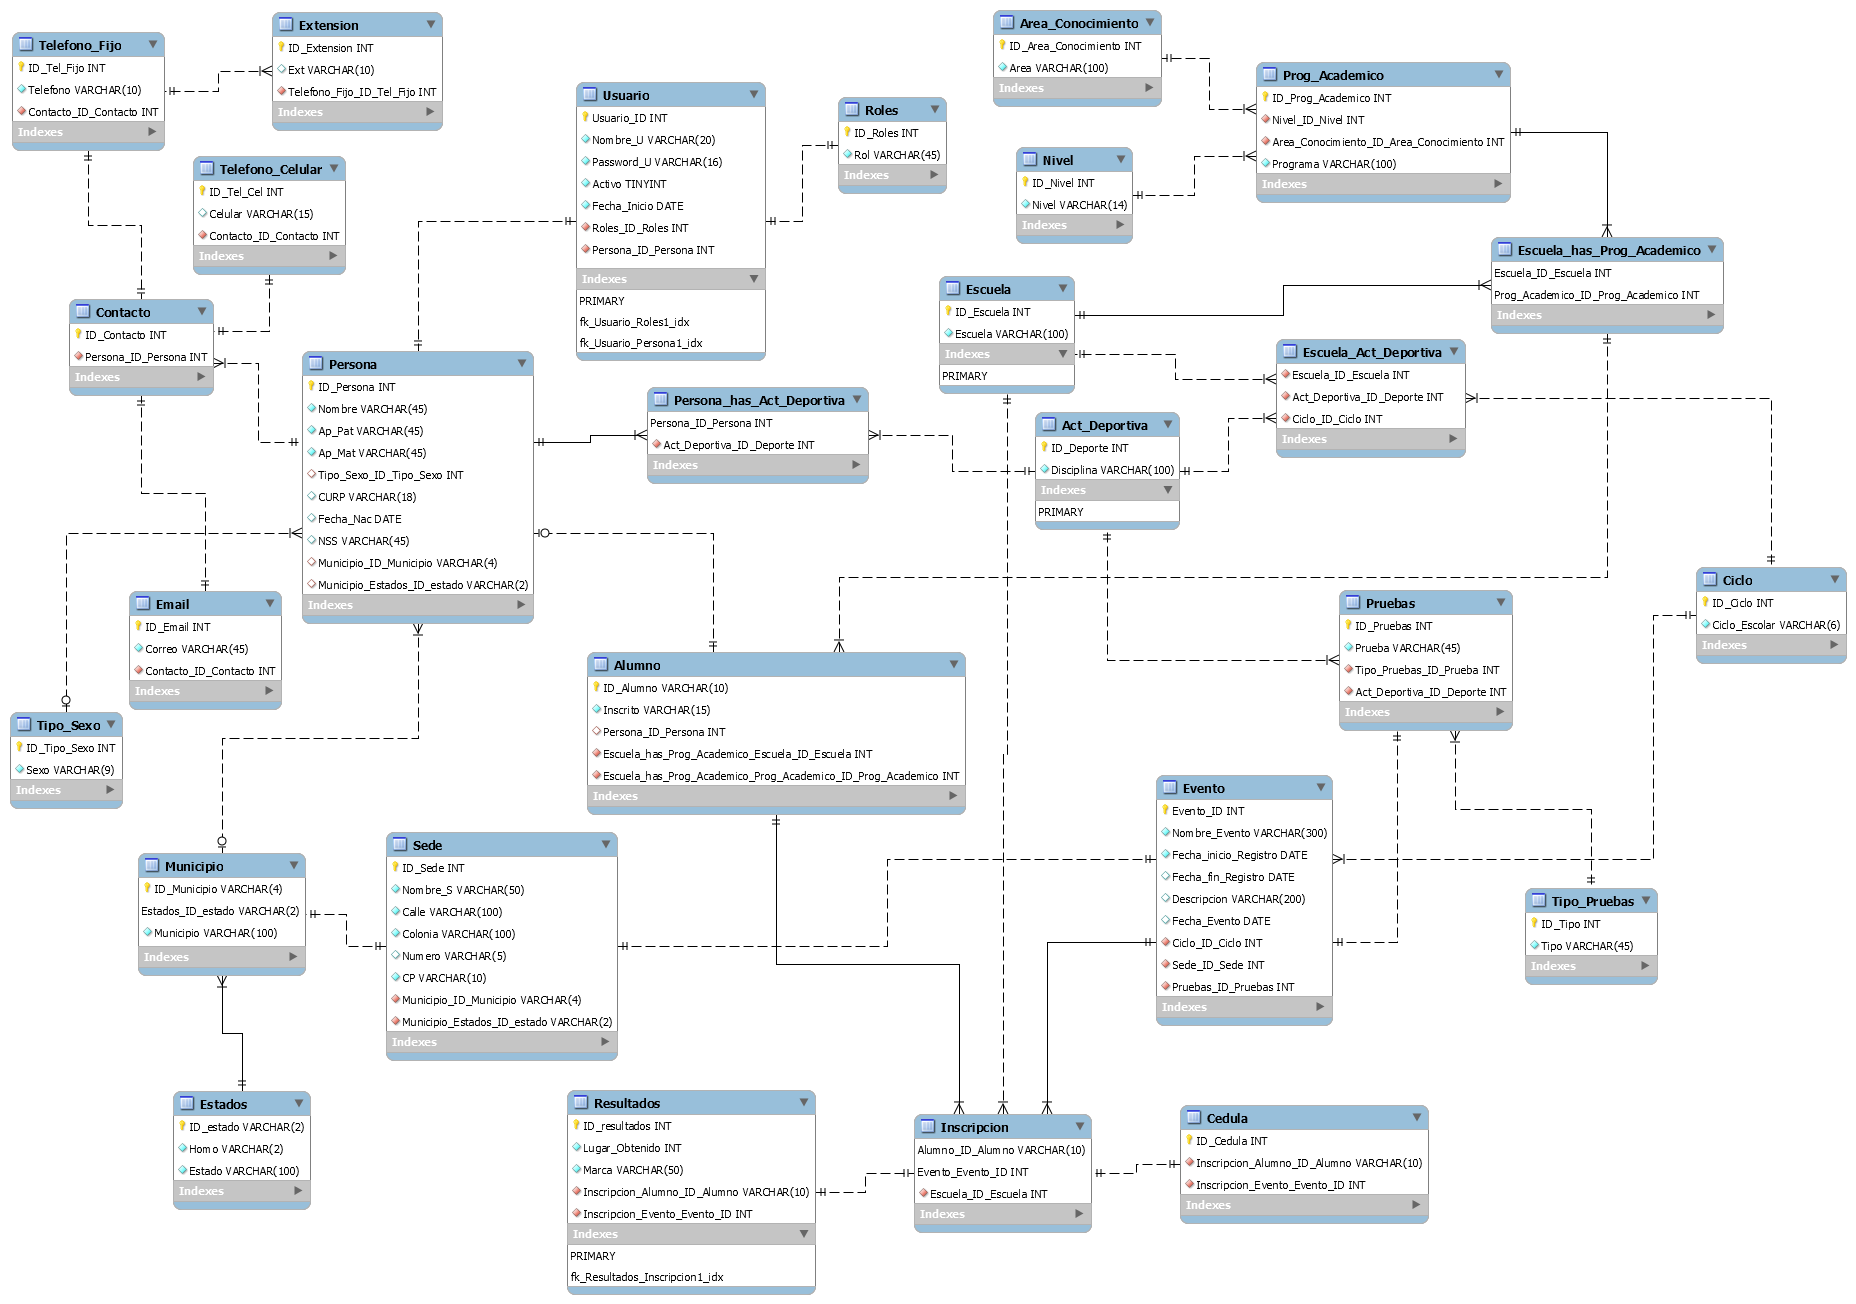
\includegraphics[angle=90, width=14cm, height=19cm]{Imagenes/RIDESCOM.png}
			\caption{Estructura de la Base de Datos de RIDESCOM}
			\label{BaseDatos}
		\end{figure}
		
		
	
	\pagebreak
		
	\chapter{Apartado I: Vistas}
		
		\begin{figure} [hbt!]
			\centering
			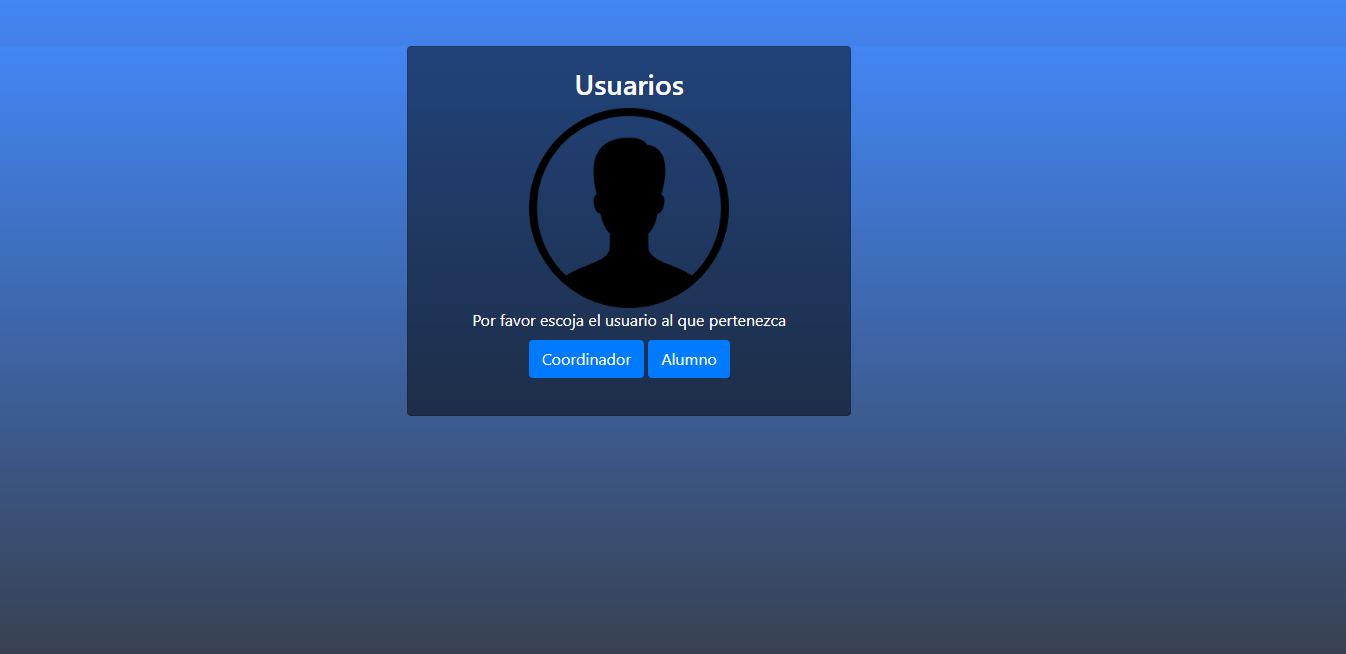
\includegraphics[width=10cm, height=6cm]{Imagenes/Vistas/VIsta1_TipoSesion}
			\caption{Vista que ayuda a definir el tipo de usuario que ingresará.}
			\label{VistaTipoSesion}
		\end{figure}
	
		\begin{figure} [hbt!]
			\centering
			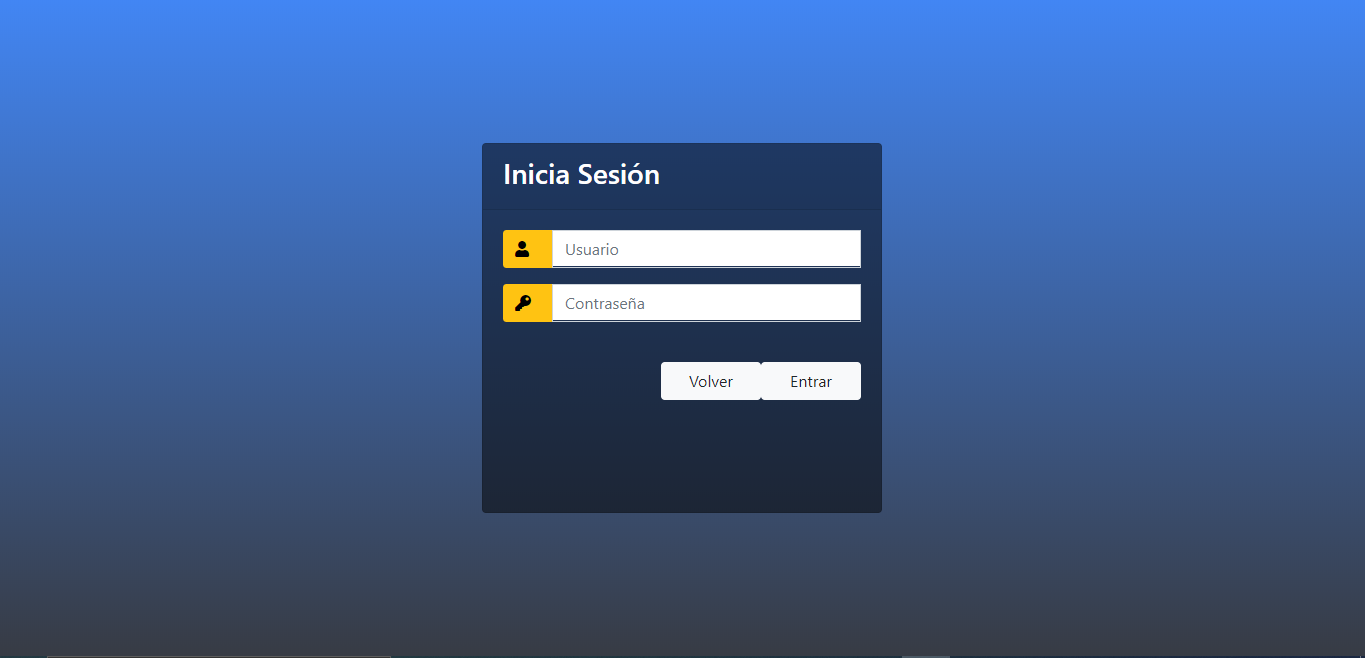
\includegraphics[width=10cm, height=6cm]{Imagenes/Vistas/Vista2_InicioSesionJFD}
			\caption{Vista del Inicio de Sesión para el Jefe de Fomento Deportivo y el Coordinador de una Unidad Académica.}
			\label{VistaInicioSesionJFD}
		\end{figure}
	
		\begin{figure} [hbt!]
			\centering
			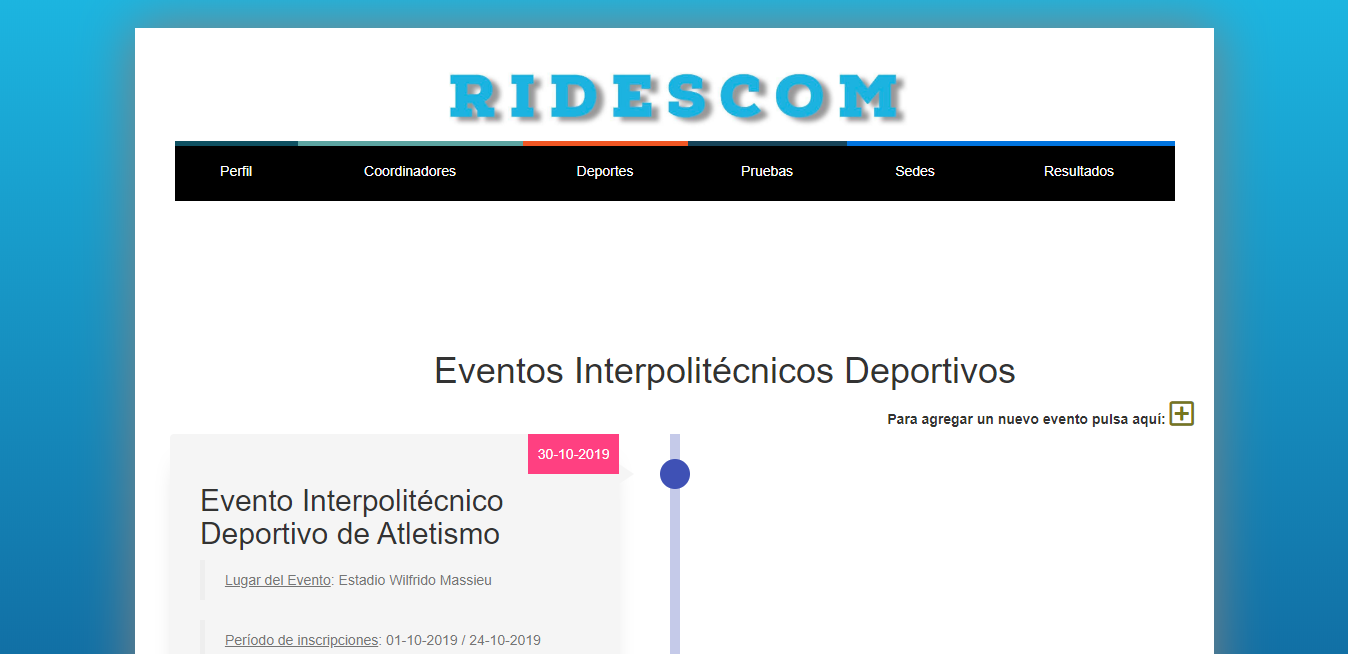
\includegraphics[width=10cm, height=6cm]{Imagenes/Vistas/Vista3_PrincipalJFD}
			\caption{Vista principal del Jefe de Fomento Deportivo (JFD).}
			\label{VistaPrincipalJFD}
		\end{figure}
			
		\begin{figure} [hbt!]
			\centering
			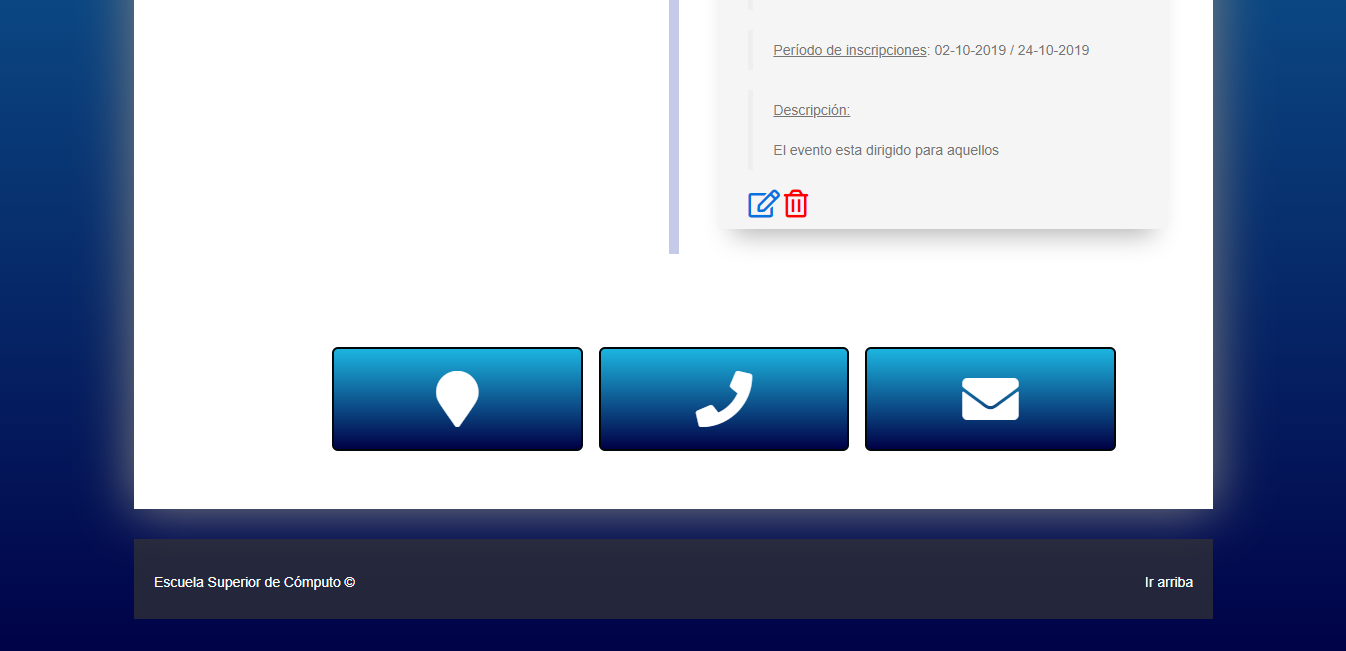
\includegraphics[width=10cm, height=6cm]{Imagenes/Vistas/Vista4_PrincipalJFD}
			\caption{Vista principal del Jefe de Fomento Deportivo continuación(JFD).}
			\label{VIstaPrincipalJFD1}
		\end{figure}
	
		\begin{figure} [hbt!]
			\centering
			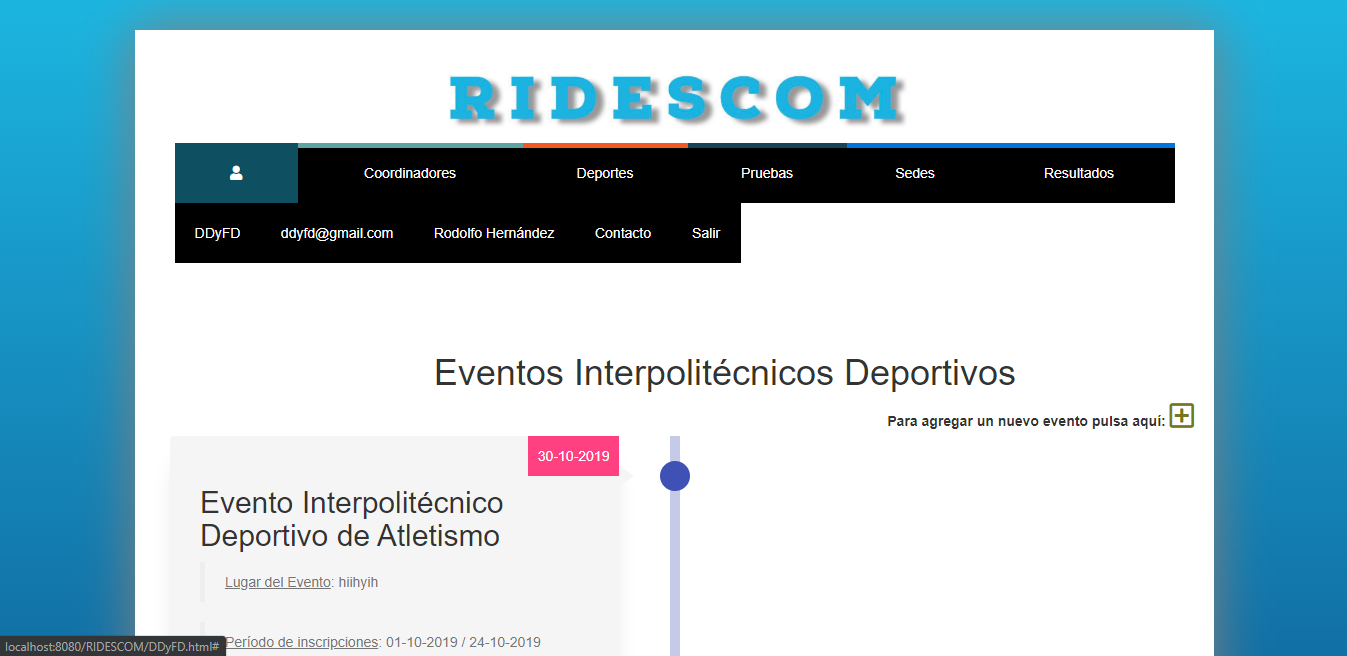
\includegraphics[width=10cm, height=6cm]{Imagenes/Vistas/Vista5_MenuUsuarioJFD}
			\caption{Vista que muestra datos del usuario en sesión.(Jefe de Fomento Deportivo)}
			\label{VistaMenuUsuario}
		\end{figure}
		
		\begin{figure} [hbt!]
			\centering
			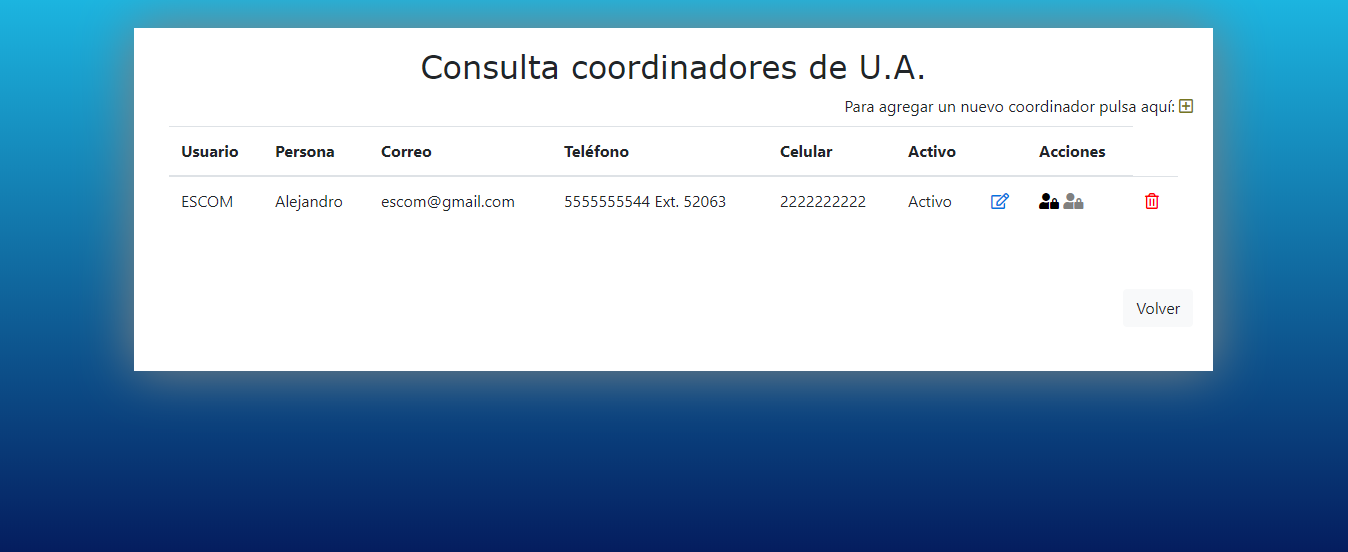
\includegraphics[width=10cm, height=6cm]{Imagenes/Vistas/Vista6_ConsultaCoordJFD}
			\caption{Vista donde se visualizan los Coordinadores de Unidades Académicas registrados.}
			\label{VistaConsultaCoord}
		\end{figure}
		
		\begin{figure} [hbt!]
			\centering
			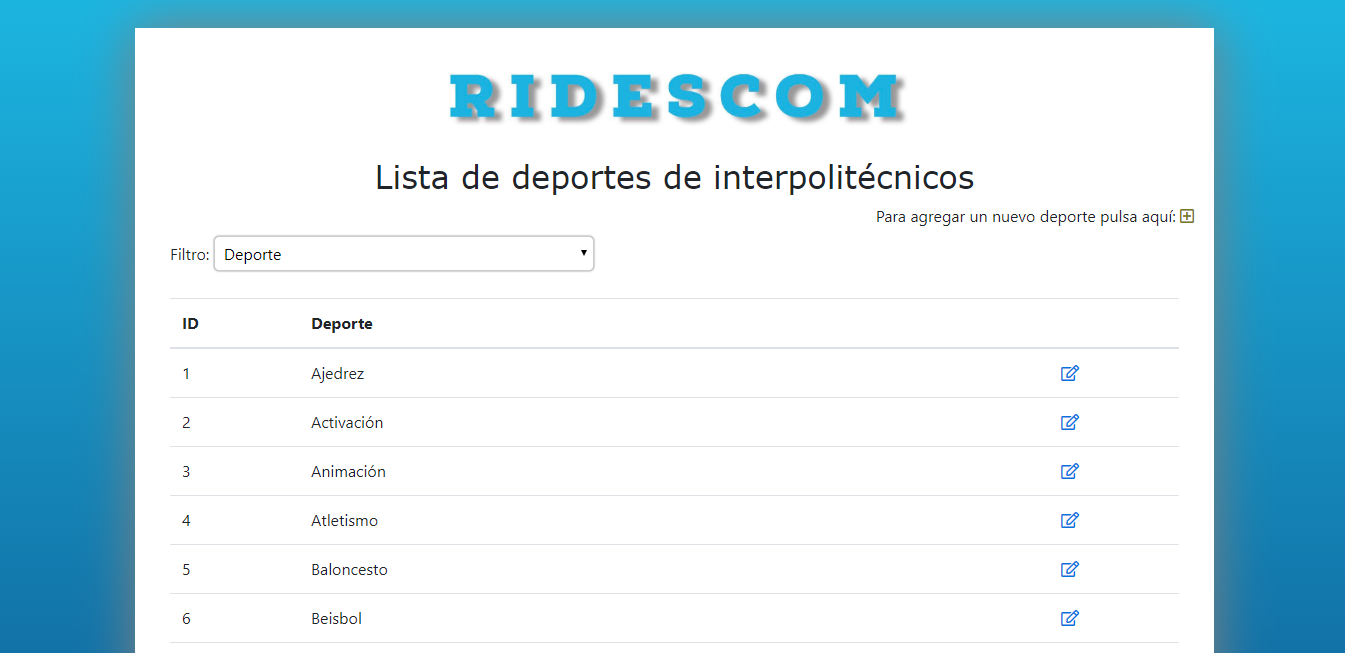
\includegraphics[width=10cm, height=6cm]{Imagenes/Vistas/Vista7_DeportesJFD}
			\caption{Vista en la que el Jefe de Fomento Deportivo visualiza los deportes que se practican actualmente en el Instituto Politécnico Nacional.}
			\label{VistaDeportes}
		\end{figure}
		
		\begin{figure} [hbt!]
			\centering
			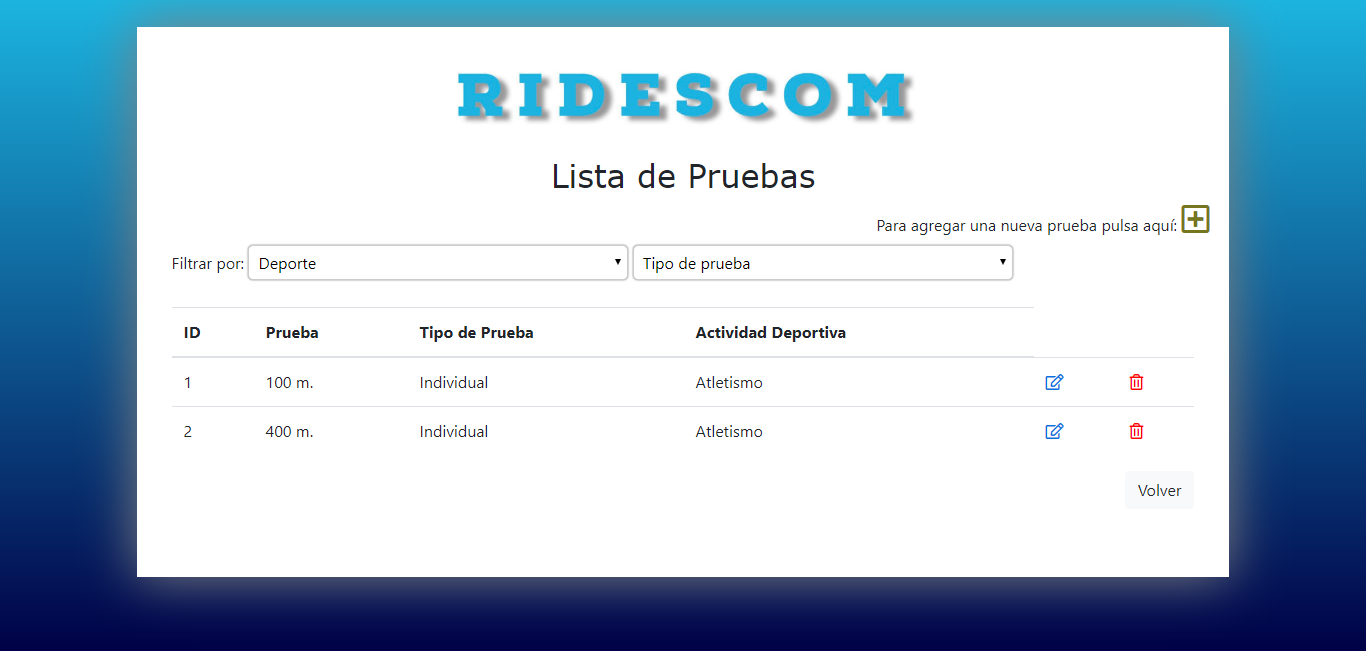
\includegraphics[width=10cm, height=6cm]{Imagenes/Vistas/Vista8_PruebaJFD}
			\caption{Vista donde el Jefe de Fomento Deportivo podrá ver las pruebas que han sido registradas.}
			\label{VistaPruebas}
		\end{figure}
	
		\begin{figure}
			\centering
			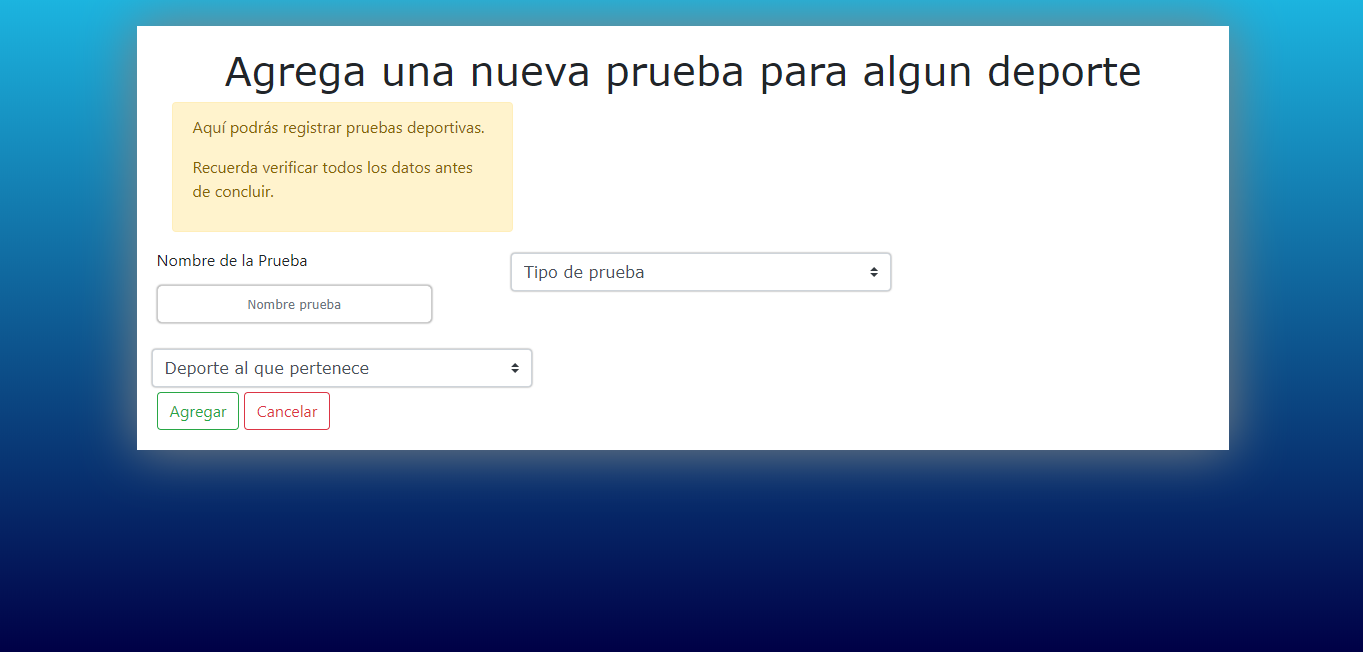
\includegraphics[width=10cm, height=6cm]{Imagenes/Vistas/Vista20_AgregaPrueba}
			\caption{Vista para agregar una prueba.}
			\label{VistaAgregaPrueba}
		\end{figure}
		
	
		\begin{figure} [hbt!]
			\centering
			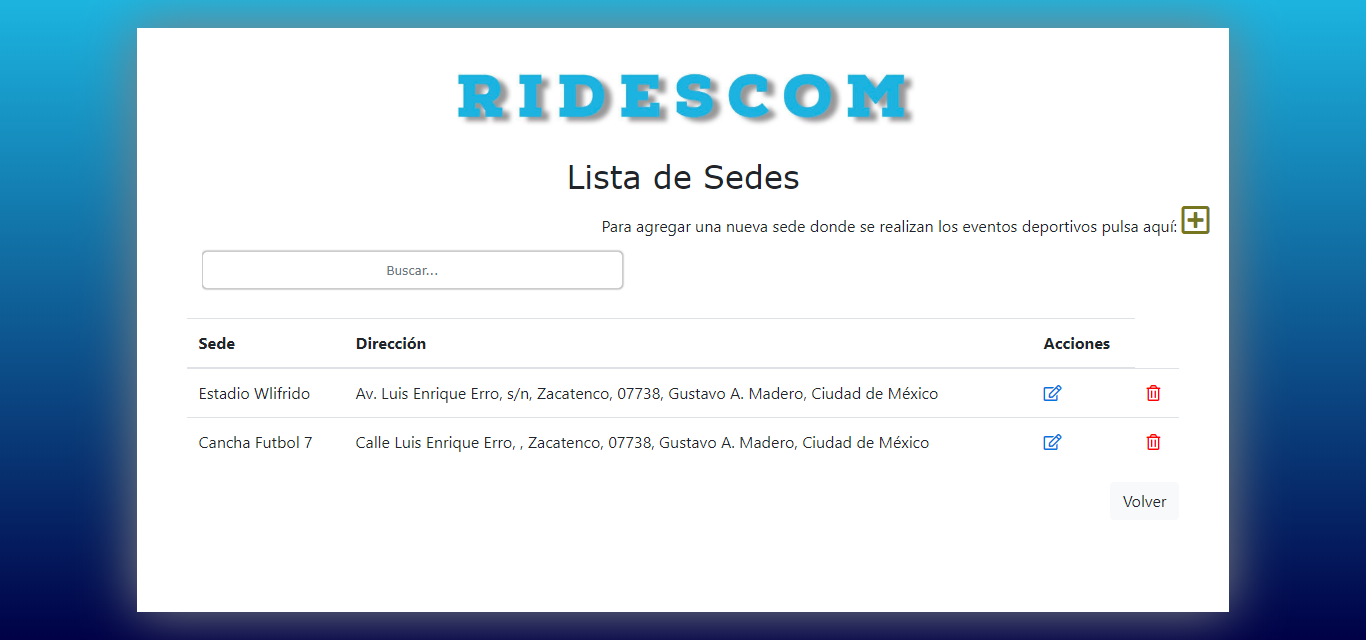
\includegraphics[width=10cm, height=6cm]{Imagenes/Vistas/Vista9_SedesJFD}
			\caption{Vista para visualizar las sedes donde se llevarán a cabo los eventos interpolitécnicos deportivos.}
			\label{VistaSedes}
		\end{figure}
		
		\begin{figure} [hbt!]
			\centering
			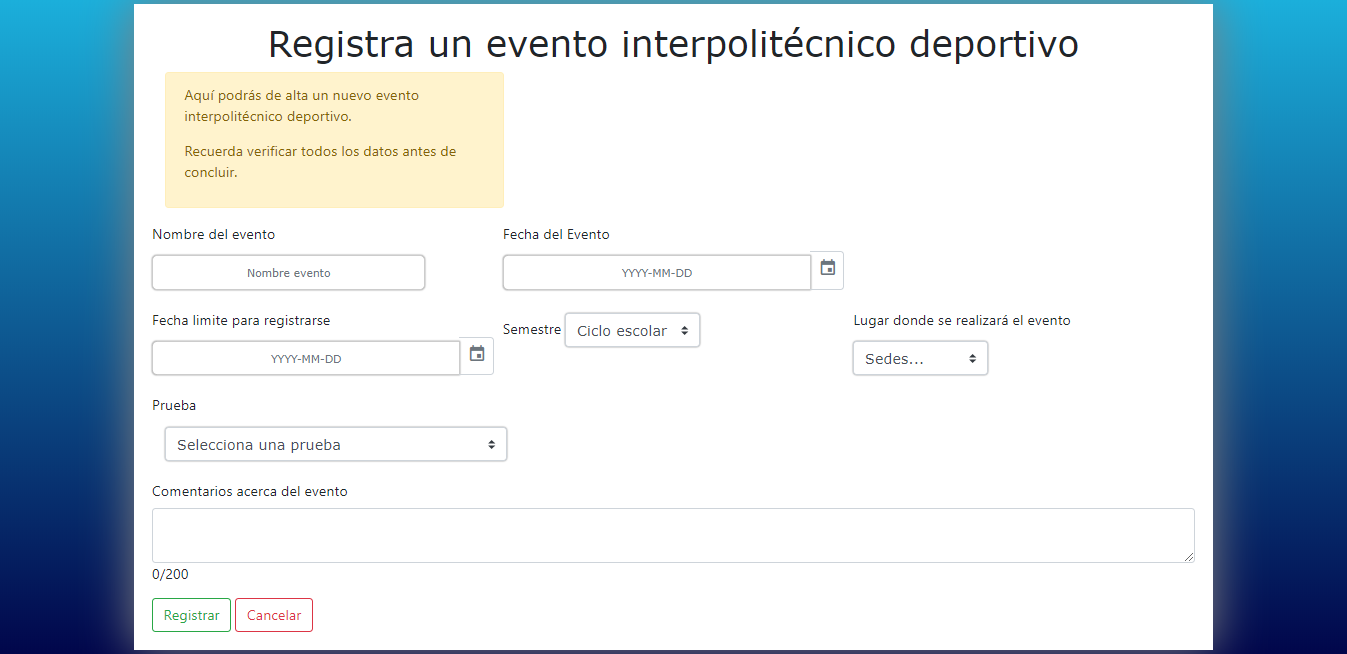
\includegraphics[width=10cm, height=6cm]{Imagenes/Vistas/Vista10_AgregaEvento}
			\caption{Vista en la que se puede agregar un Evento Interpolitécnico Deportivo.}
			\label{VistaAgregarEvento}
		\end{figure}
	
		\begin{figure} [hbt!]
			\centering
			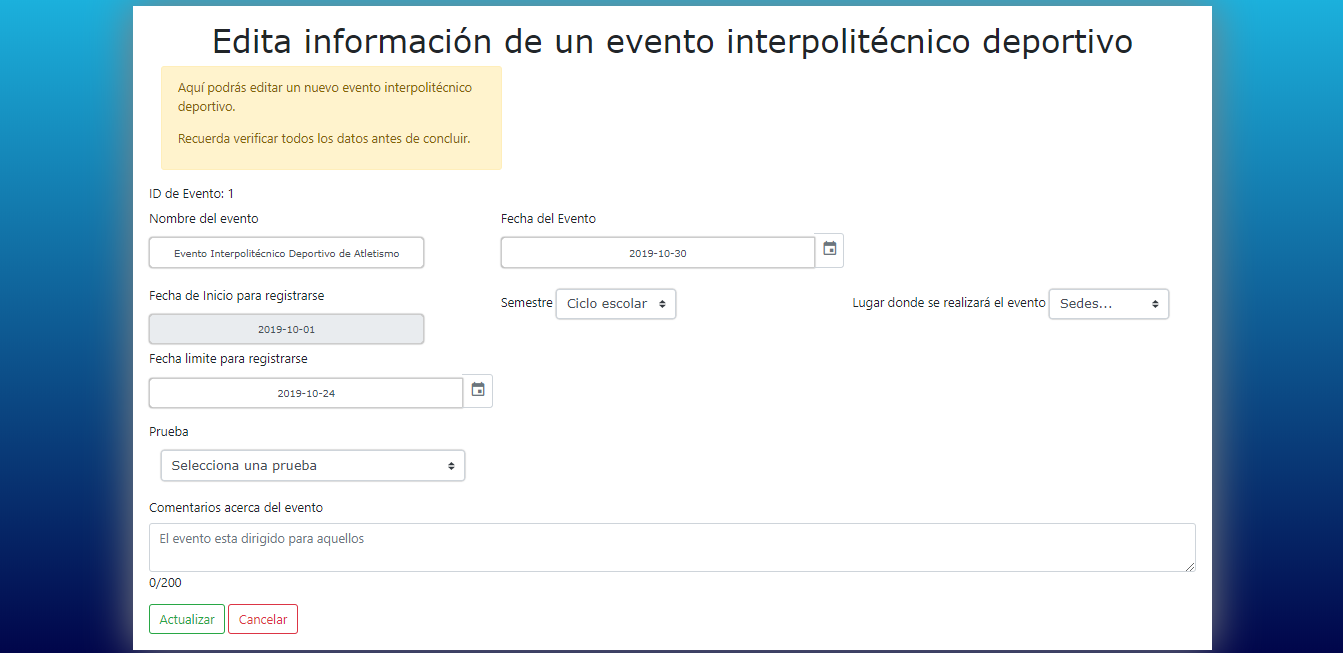
\includegraphics[width=10cm, height=6cm]{Imagenes/Vistas/Vista11_EditarEvento}
			\caption{Vista en la que se pueden editar los datos de un Evento Interpolitécnico Deportivo.}
			\label{VistaEditarEvento}
		\end{figure}
		
		\begin{figure} [hbt!]
			\centering
			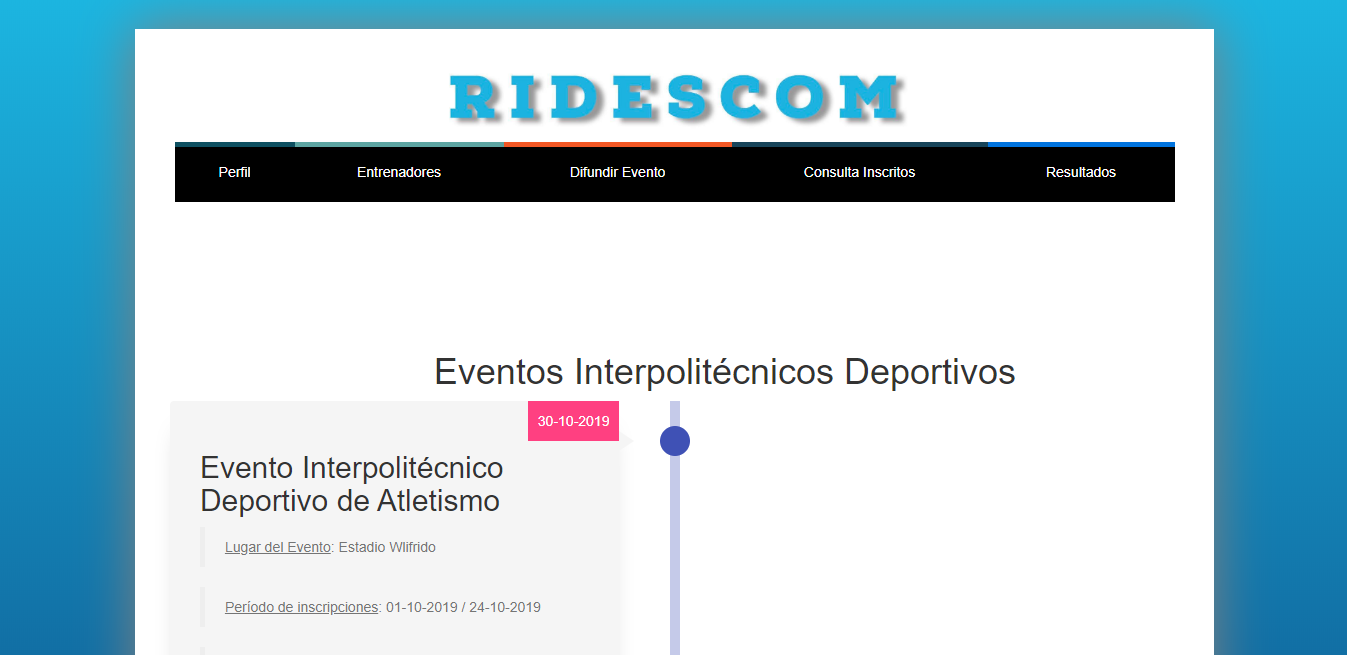
\includegraphics[width=10cm, height=6cm]{Imagenes/Vistas/Vista12_PrincipalCoord}
			\caption{Vista principal del Coordinador de la Unidad Académica.}
			\label{VistaPrincipalCoord}
		\end{figure}
		
		\begin{figure} [hbt!]
			\centering
			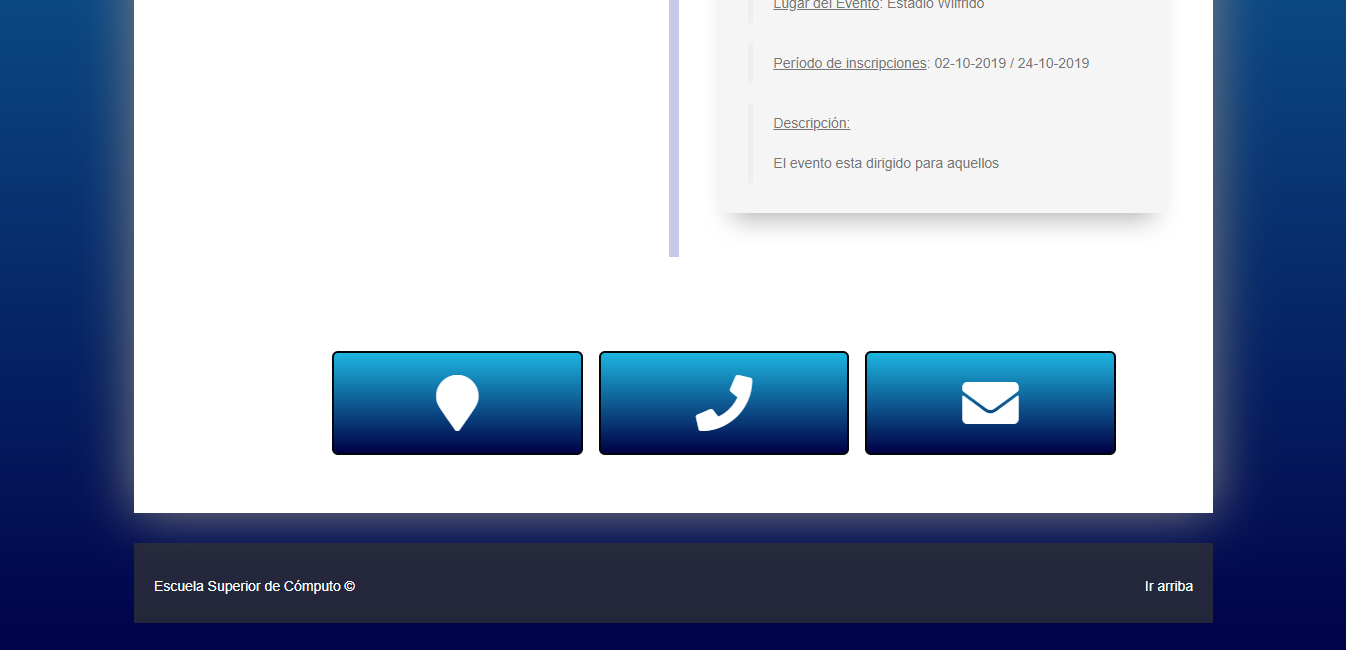
\includegraphics[width=10cm, height=6cm]{Imagenes/Vistas/Vista13_PrincipalCoord}
			\caption{Vistas principal del Coordinador de la Unidad Académica. (Continuación)}
			\label{VistaPrincipalCoord1}
		\end{figure}
		
		\begin{figure} [hbt!]
			\centering
			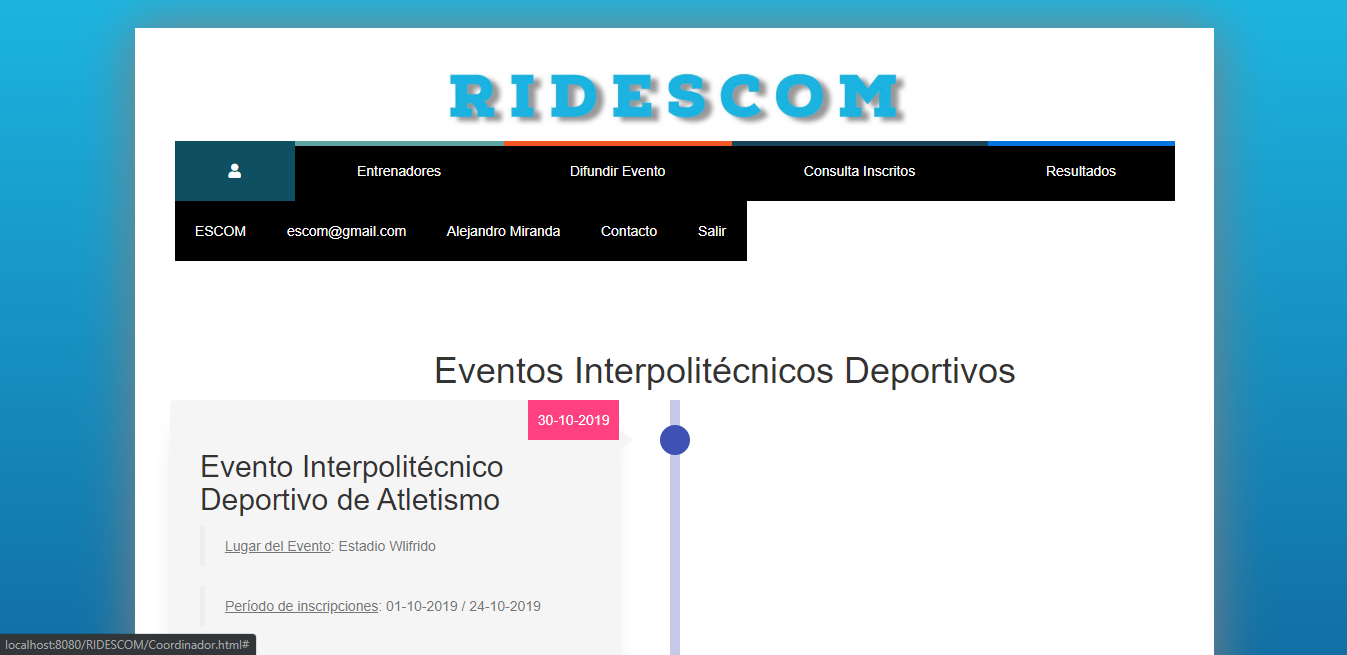
\includegraphics[width=10cm, height=6cm]{Imagenes/Vistas/Vista14_MenuUsuarioCoord}
			\caption{Vista que muestra datos del usuario en sesión.(Coordinador)}
			\label{VistaMenuCoord}
		\end{figure}
		
		\begin{figure} [hbt!]
			\centering
			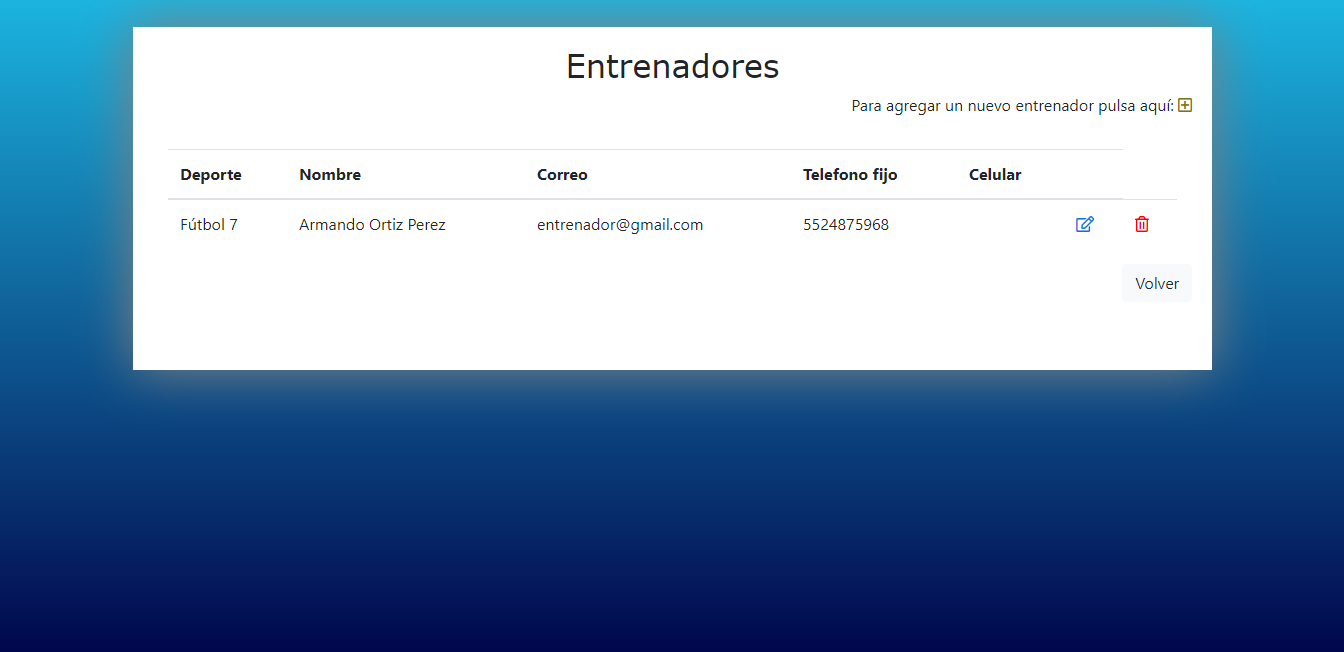
\includegraphics[width=10cm, height=6cm]{Imagenes/Vistas/Vista15_ConsultaEntrenador}
			\caption{Vista para la consulta de entrenadores.}
			\label{VistaConsultaEntrenador}
		\end{figure}
		
		\begin{figure} [hbt!]
			\centering
			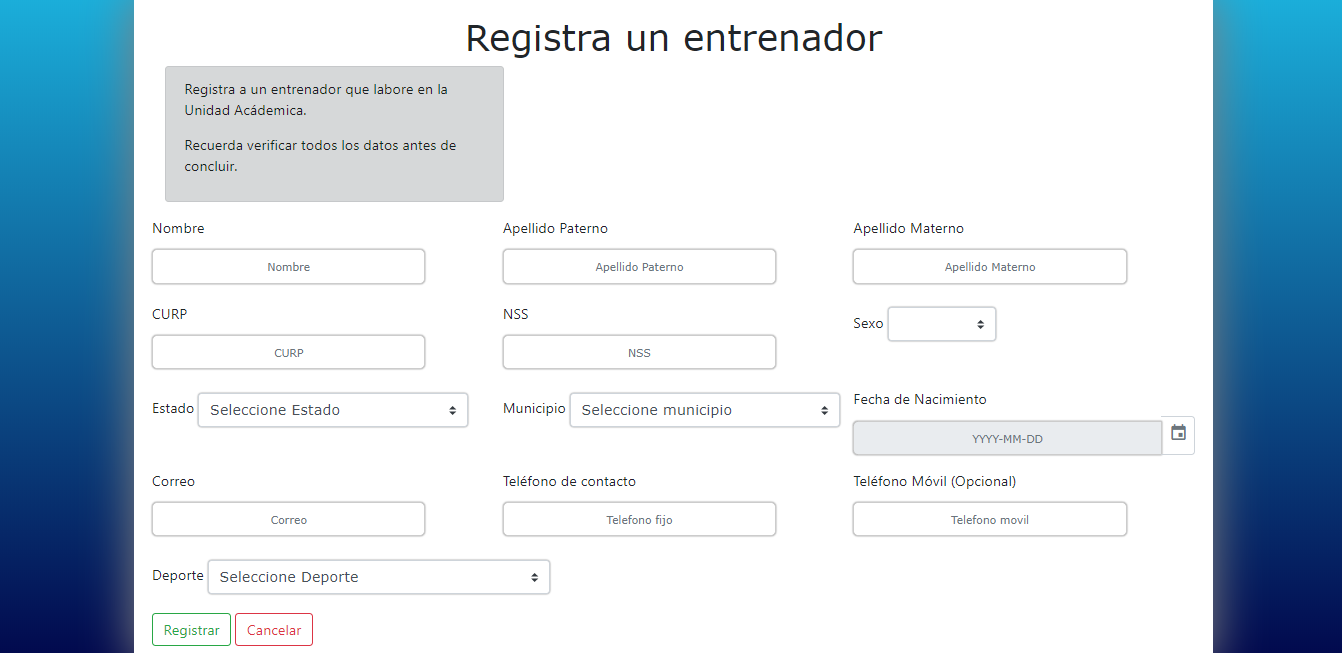
\includegraphics[width=10cm, height=6cm]{Imagenes/Vistas/Vista16_AgregaEntrenador}
			\caption{Vista para agregar a un entrenador.}
			\label{VistaAgregarEntrenador}
		\end{figure}
	
		\begin{figure} [hbt!]
			\centering
			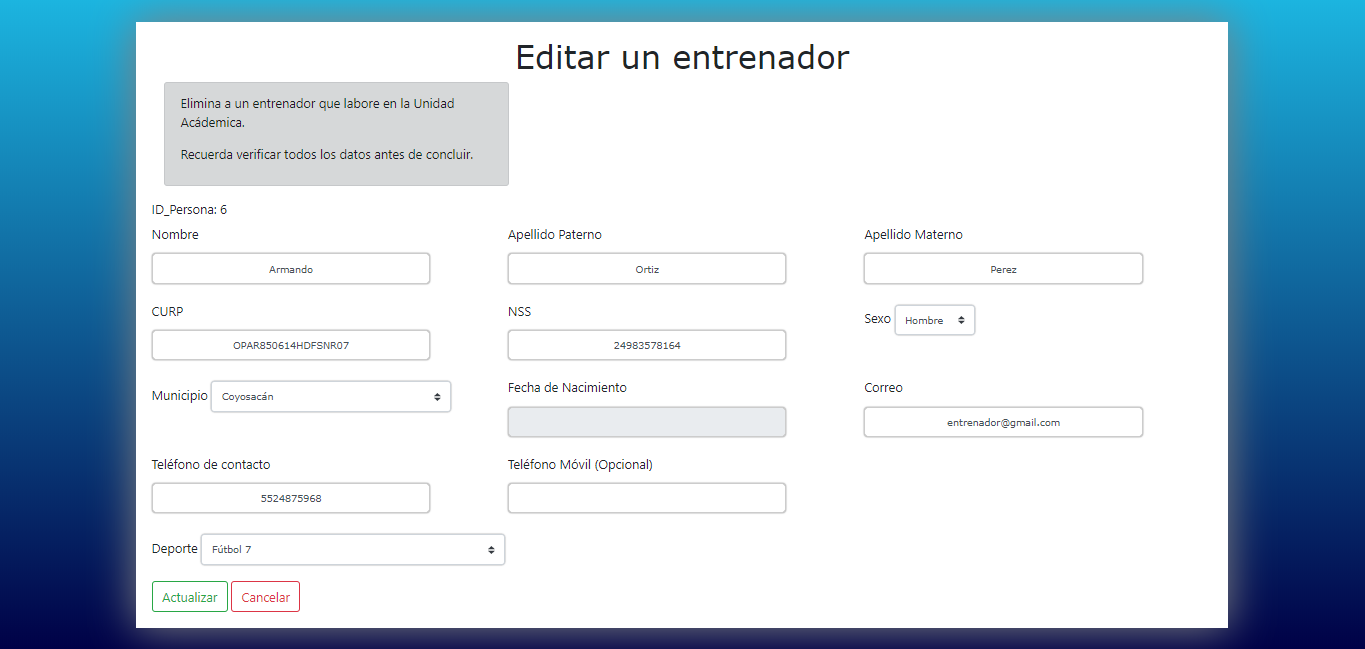
\includegraphics[width=10cm, height=6cm]{Imagenes/Vistas/Vista17_EditarEntrenador}
			\caption{Vista para editar los datos del entrenador.}
			\label{VistaEditarEntrenador}
		\end{figure}
		
		\begin{figure} [hbt!]
			\centering
			\includegraphics[width=10cm, height=6cm]{Imagenes/Vistas/Vista18_ConsultaInscritos}
			\caption{Vista para consultar los alumnos inscritos en algún Evento Interpolitécnico Deportivo.}
			\label{VistaConsultaInscritos}
		\end{figure}
		
		\begin{figure} [hbt!]
			\centering
			\includegraphics[width=10cm, height=6cm]{Imagenes/Vistas/Vista19_ConsultaResultados}
			\caption{Vista para consultar los resultados obtenidos por los participantes.}
			\label{VistaConsultaResultados}
		\end{figure}
				
		\chapter{Apartado J: API Facebook}
		La implementación de la API de Facebook al proyecto a sido de difícil implementación, ya que
		
		
